\documentclass[twoside]{book}

% Packages required by doxygen
\usepackage{fixltx2e}
\usepackage{calc}
\usepackage{doxygen}
\usepackage[export]{adjustbox} % also loads graphicx
\usepackage{graphicx}
\usepackage[utf8]{inputenc}
\usepackage{makeidx}
\usepackage{multicol}
\usepackage{multirow}
\PassOptionsToPackage{warn}{textcomp}
\usepackage{textcomp}
\usepackage[nointegrals]{wasysym}
\usepackage[table]{xcolor}

% NLS support packages
\usepackage[T2A]{fontenc}
\usepackage[russian]{babel}

% Font selection
\usepackage[T1]{fontenc}
\usepackage[scaled=.90]{helvet}
\usepackage{courier}
\usepackage{amssymb}
\usepackage{sectsty}
\renewcommand{\familydefault}{\sfdefault}
\allsectionsfont{%
  \fontseries{bc}\selectfont%
  \color{darkgray}%
}
\renewcommand{\DoxyLabelFont}{%
  \fontseries{bc}\selectfont%
  \color{darkgray}%
}
\newcommand{\+}{\discretionary{\mbox{\scriptsize$\hookleftarrow$}}{}{}}

% Page & text layout
\usepackage{geometry}
\geometry{%
  a4paper,%
  top=2.5cm,%
  bottom=2.5cm,%
  left=2.5cm,%
  right=2.5cm%
}
\tolerance=750
\hfuzz=15pt
\hbadness=750
\setlength{\emergencystretch}{15pt}
\setlength{\parindent}{0cm}
\setlength{\parskip}{3ex plus 2ex minus 2ex}
\makeatletter
\renewcommand{\paragraph}{%
  \@startsection{paragraph}{4}{0ex}{-1.0ex}{1.0ex}{%
    \normalfont\normalsize\bfseries\SS@parafont%
  }%
}
\renewcommand{\subparagraph}{%
  \@startsection{subparagraph}{5}{0ex}{-1.0ex}{1.0ex}{%
    \normalfont\normalsize\bfseries\SS@subparafont%
  }%
}
\makeatother

% Headers & footers
\usepackage{fancyhdr}
\pagestyle{fancyplain}
\fancyhead[LE]{\fancyplain{}{\bfseries\thepage}}
\fancyhead[CE]{\fancyplain{}{}}
\fancyhead[RE]{\fancyplain{}{\bfseries\leftmark}}
\fancyhead[LO]{\fancyplain{}{\bfseries\rightmark}}
\fancyhead[CO]{\fancyplain{}{}}
\fancyhead[RO]{\fancyplain{}{\bfseries\thepage}}
\fancyfoot[LE]{\fancyplain{}{}}
\fancyfoot[CE]{\fancyplain{}{}}
\fancyfoot[RE]{\fancyplain{}{\bfseries\scriptsize Создано системой Doxygen }}
\fancyfoot[LO]{\fancyplain{}{\bfseries\scriptsize Создано системой Doxygen }}
\fancyfoot[CO]{\fancyplain{}{}}
\fancyfoot[RO]{\fancyplain{}{}}
\renewcommand{\footrulewidth}{0.4pt}
\renewcommand{\chaptermark}[1]{%
  \markboth{#1}{}%
}
\renewcommand{\sectionmark}[1]{%
  \markright{\thesection\ #1}%
}

% Indices & bibliography
\usepackage{natbib}
\usepackage[titles]{tocloft}
\setcounter{tocdepth}{3}
\setcounter{secnumdepth}{5}
\makeindex

% Hyperlinks (required, but should be loaded last)
\usepackage{ifpdf}
\ifpdf
  \usepackage[pdftex,pagebackref=true]{hyperref}
\else
  \usepackage[ps2pdf,pagebackref=true]{hyperref}
\fi
\hypersetup{%
  colorlinks=true,%
  linkcolor=blue,%
  citecolor=blue,%
  unicode%
}

% Custom commands
\newcommand{\clearemptydoublepage}{%
  \newpage{\pagestyle{empty}\cleardoublepage}%
}

\usepackage{caption}
\captionsetup{labelsep=space,justification=centering,font={bf},singlelinecheck=off,skip=4pt,position=top}

%===== C O N T E N T S =====

\begin{document}

% Titlepage & ToC
\hypersetup{pageanchor=false,
             bookmarksnumbered=true,
             pdfencoding=unicode
            }
\pagenumbering{alph}
\begin{titlepage}
\vspace*{7cm}
\begin{center}%
{\Large C\+W\+\_\+\+Interpreter\+VM }\\
\vspace*{1cm}
{\large Создано системой Doxygen 1.8.12}\\
\end{center}
\end{titlepage}
\clearemptydoublepage
\pagenumbering{roman}
\tableofcontents
\clearemptydoublepage
\pagenumbering{arabic}
\hypersetup{pageanchor=true}

%--- Begin generated contents ---
\chapter{Алфавитный указатель пространств имен}
\section{Пространства имен}
Полный список документированных пространств имен.\begin{DoxyCompactList}
\item\contentsline{section}{\hyperlink{namespace_ui}{Ui} \\*пространство имён формы QT }{\pageref{namespace_ui}}{}
\end{DoxyCompactList}

\chapter{Иерархический список классов}
\section{Иерархия классов}
Иерархия классов.\begin{DoxyCompactList}
\item \contentsline{section}{Computer\+:\+:bits}{\pageref{struct_computer_1_1bits}}{}
\item \contentsline{section}{Command}{\pageref{class_command}}{}
\begin{DoxyCompactList}
\item \contentsline{section}{c\+Iadd}{\pageref{classc_iadd}}{}
\item \contentsline{section}{c\+Icmp}{\pageref{classc_icmp}}{}
\item \contentsline{section}{c\+Idiv}{\pageref{classc_idiv}}{}
\item \contentsline{section}{c\+Iin}{\pageref{classc_iin}}{}
\item \contentsline{section}{c\+Imod}{\pageref{classc_imod}}{}
\item \contentsline{section}{c\+Imul}{\pageref{classc_imul}}{}
\item \contentsline{section}{c\+Iout}{\pageref{classc_iout}}{}
\item \contentsline{section}{c\+Isub}{\pageref{classc_isub}}{}
\item \contentsline{section}{c\+JG}{\pageref{classc_j_g}}{}
\item \contentsline{section}{c\+JL}{\pageref{classc_j_l}}{}
\item \contentsline{section}{c\+Jmp}{\pageref{classc_jmp}}{}
\item \contentsline{section}{c\+JZ}{\pageref{classc_j_z}}{}
\item \contentsline{section}{c\+Load}{\pageref{classc_load}}{}
\item \contentsline{section}{c\+Radd}{\pageref{classc_radd}}{}
\item \contentsline{section}{c\+Radr}{\pageref{classc_radr}}{}
\item \contentsline{section}{c\+Rcmp}{\pageref{classc_rcmp}}{}
\item \contentsline{section}{c\+Rdiv}{\pageref{classc_rdiv}}{}
\item \contentsline{section}{c\+Rin}{\pageref{classc_rin}}{}
\item \contentsline{section}{c\+Rmul}{\pageref{classc_rmul}}{}
\item \contentsline{section}{c\+Rout}{\pageref{classc_rout}}{}
\item \contentsline{section}{c\+Rsub}{\pageref{classc_rsub}}{}
\item \contentsline{section}{c\+S\+T\+OP}{\pageref{classc_s_t_o_p}}{}
\item \contentsline{section}{c\+Store}{\pageref{classc_store}}{}
\end{DoxyCompactList}
\item \contentsline{section}{Computer\+:\+:command}{\pageref{struct_computer_1_1command}}{}
\item \contentsline{section}{Computer}{\pageref{class_computer}}{}
\item \contentsline{section}{Computer\+:\+:data}{\pageref{union_computer_1_1data}}{}
\item Q\+Main\+Window\begin{DoxyCompactList}
\item \contentsline{section}{Main\+Window}{\pageref{class_main_window}}{}
\end{DoxyCompactList}
\item Q\+Object\begin{DoxyCompactList}
\item \contentsline{section}{interpreter}{\pageref{classinterpreter}}{}
\end{DoxyCompactList}
\end{DoxyCompactList}

\chapter{Алфавитный указатель классов}
\section{Классы}
Классы с их кратким описанием.\begin{DoxyCompactList}
\item\contentsline{section}{\hyperlink{struct_computer_1_1bits}{Computer\+::bits} \\*P\+SW (Cостояние процессора) }{\pageref{struct_computer_1_1bits}}{}
\item\contentsline{section}{\hyperlink{classc_iadd}{c\+Iadd} \\*Сложение целых чисел }{\pageref{classc_iadd}}{}
\item\contentsline{section}{\hyperlink{classc_icmp}{c\+Icmp} \\*Сравнение целых }{\pageref{classc_icmp}}{}
\item\contentsline{section}{\hyperlink{classc_idiv}{c\+Idiv} \\*Деление целых чисел }{\pageref{classc_idiv}}{}
\item\contentsline{section}{\hyperlink{classc_iin}{c\+Iin} \\*Ввод целого }{\pageref{classc_iin}}{}
\item\contentsline{section}{\hyperlink{classc_imod}{c\+Imod} \\*Остаток от деления целых чисел }{\pageref{classc_imod}}{}
\item\contentsline{section}{\hyperlink{classc_imul}{c\+Imul} \\*Умножение целых чисел }{\pageref{classc_imul}}{}
\item\contentsline{section}{\hyperlink{classc_iout}{c\+Iout} \\*вывод целого }{\pageref{classc_iout}}{}
\item\contentsline{section}{\hyperlink{classc_isub}{c\+Isub} \\*Вычитание целых чисел }{\pageref{classc_isub}}{}
\item\contentsline{section}{\hyperlink{classc_j_g}{c\+JG} \\*переход, если больше }{\pageref{classc_j_g}}{}
\item\contentsline{section}{\hyperlink{classc_j_l}{c\+JL} \\*переход, если меньше }{\pageref{classc_j_l}}{}
\item\contentsline{section}{\hyperlink{classc_jmp}{c\+Jmp} \\*Безусловный переход }{\pageref{classc_jmp}}{}
\item\contentsline{section}{\hyperlink{classc_j_z}{c\+JZ} \\*переход, если ноль (равны) }{\pageref{classc_j_z}}{}
\item\contentsline{section}{\hyperlink{classc_load}{c\+Load} \\*Загрузка сумматора }{\pageref{classc_load}}{}
\item\contentsline{section}{\hyperlink{class_command}{Command} \\*Базовый абстрактный класс для паттерна \char`\"{}Комманда\char`\"{} }{\pageref{class_command}}{}
\item\contentsline{section}{\hyperlink{struct_computer_1_1command}{Computer\+::command} \\*\hyperlink{class_command}{Command} struct -\/ структура команды для выполнения. 3 байта }{\pageref{struct_computer_1_1command}}{}
\item\contentsline{section}{\hyperlink{class_computer}{Computer} \\*Класс \hyperlink{class_computer}{Computer} реализует архитектуру компьютера }{\pageref{class_computer}}{}
\item\contentsline{section}{\hyperlink{classc_radd}{c\+Radd} \\*Сложение дробных чисел }{\pageref{classc_radd}}{}
\item\contentsline{section}{\hyperlink{classc_radr}{c\+Radr} \\*Загрузка адрессного регистра }{\pageref{classc_radr}}{}
\item\contentsline{section}{\hyperlink{classc_rcmp}{c\+Rcmp} \\*Сравнение вещественных }{\pageref{classc_rcmp}}{}
\item\contentsline{section}{\hyperlink{classc_rdiv}{c\+Rdiv} \\*Деление дробных чисел }{\pageref{classc_rdiv}}{}
\item\contentsline{section}{\hyperlink{classc_rin}{c\+Rin} \\*Ввод вещественного }{\pageref{classc_rin}}{}
\item\contentsline{section}{\hyperlink{classc_rmul}{c\+Rmul} \\*Умножение дробных чисел }{\pageref{classc_rmul}}{}
\item\contentsline{section}{\hyperlink{classc_rout}{c\+Rout} \\*Вывод вещественного }{\pageref{classc_rout}}{}
\item\contentsline{section}{\hyperlink{classc_rsub}{c\+Rsub} \\*Вычитание дробных чисел }{\pageref{classc_rsub}}{}
\item\contentsline{section}{\hyperlink{classc_s_t_o_p}{c\+S\+T\+OP} \\*СТОП }{\pageref{classc_s_t_o_p}}{}
\item\contentsline{section}{\hyperlink{classc_store}{c\+Store} \\*Выгрузка сумматора }{\pageref{classc_store}}{}
\item\contentsline{section}{\hyperlink{union_computer_1_1data}{Computer\+::data} \\*Data union -\/ структура данных 4 байта }{\pageref{union_computer_1_1data}}{}
\item\contentsline{section}{\hyperlink{classinterpreter}{interpreter} \\*The interpreter class }{\pageref{classinterpreter}}{}
\item\contentsline{section}{\hyperlink{class_main_window}{Main\+Window} \\*
\begin{DoxyItemize}
\item G\+UI форма программы 
\end{DoxyItemize}}{\pageref{class_main_window}}{}
\end{DoxyCompactList}

\chapter{Пространства имен}
\hypertarget{namespace_ui}{}\section{Пространство имен Ui}
\label{namespace_ui}\index{Ui@{Ui}}


пространство имён формы QT.  




\subsection{Подробное описание}
пространство имён формы QT. 
\chapter{Классы}
\hypertarget{struct_computer_1_1bits}{}\section{Структура Computer\+:\+:bits}
\label{struct_computer_1_1bits}\index{Computer\+::bits@{Computer\+::bits}}


P\+SW (Cостояние процессора)  


\subsection*{Открытые атрибуты}
\begin{DoxyCompactItemize}
\item 
\hypertarget{struct_computer_1_1bits_a7781883b446209714ad687e2a4f77526}{}\label{struct_computer_1_1bits_a7781883b446209714ad687e2a4f77526} 
address \hyperlink{struct_computer_1_1bits_a7781883b446209714ad687e2a4f77526}{IP}
\begin{DoxyCompactList}\small\item\em Instruction Pointer. \end{DoxyCompactList}\item 
\hypertarget{struct_computer_1_1bits_a74cfe87f17ba348db37c74bbd5e56828}{}\label{struct_computer_1_1bits_a74cfe87f17ba348db37c74bbd5e56828} 
bit \hyperlink{struct_computer_1_1bits_a74cfe87f17ba348db37c74bbd5e56828}{SF}\+:1
\begin{DoxyCompactList}\small\item\em Sign flag результат положительный -\/ 1. \end{DoxyCompactList}\item 
\hypertarget{struct_computer_1_1bits_a5307edeadd212f1fc19e9f6f5346df39}{}\label{struct_computer_1_1bits_a5307edeadd212f1fc19e9f6f5346df39} 
bit \hyperlink{struct_computer_1_1bits_a5307edeadd212f1fc19e9f6f5346df39}{ZF}\+:1
\begin{DoxyCompactList}\small\item\em Zero flag Резульат равен нулю -\/ 1. \end{DoxyCompactList}\item 
\hypertarget{struct_computer_1_1bits_aaec5be5e3ab9ea9aa4b1672af9e26312}{}\label{struct_computer_1_1bits_aaec5be5e3ab9ea9aa4b1672af9e26312} 
bit \hyperlink{struct_computer_1_1bits_aaec5be5e3ab9ea9aa4b1672af9e26312}{OF}\+:1
\begin{DoxyCompactList}\small\item\em Overflow flag переполнение \end{DoxyCompactList}\item 
\hypertarget{struct_computer_1_1bits_a40e6b988a2d0d733a19c3f75fad8a348}{}\label{struct_computer_1_1bits_a40e6b988a2d0d733a19c3f75fad8a348} 
bit \hyperlink{struct_computer_1_1bits_a40e6b988a2d0d733a19c3f75fad8a348}{\+\_\+\+\_\+pad0\+\_\+\+\_\+}\+:13
\begin{DoxyCompactList}\small\item\em не используется \end{DoxyCompactList}\end{DoxyCompactItemize}


\subsection{Подробное описание}
P\+SW (Cостояние процессора) 

Объявления и описания членов структуры находятся в файле\+:\begin{DoxyCompactItemize}
\item 
C\+:/\+Users/sstarkov/\+Documents/kr\+\_\+\+Interpreter\+V\+M/sources/computer.\+h\end{DoxyCompactItemize}

\hypertarget{classc_iadd}{}\section{Класс c\+Iadd}
\label{classc_iadd}\index{c\+Iadd@{c\+Iadd}}


Сложение целых чисел  




{\ttfamily \#include $<$command.\+h$>$}

Граф наследования\+:c\+Iadd\+:\begin{figure}[H]
\begin{center}
\leavevmode
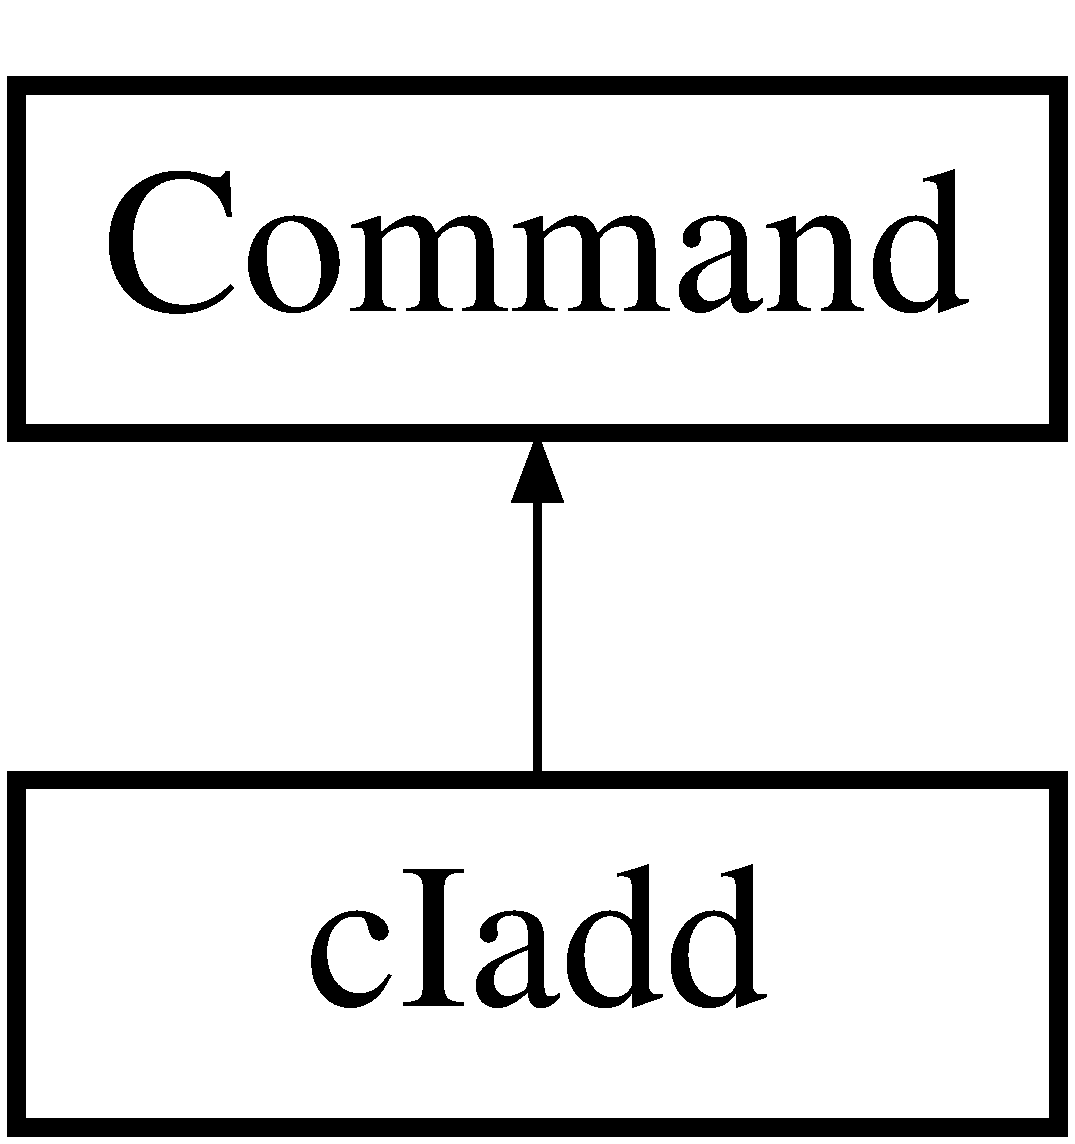
\includegraphics[height=2.000000cm]{classc_iadd}
\end{center}
\end{figure}
\subsection*{Открытые члены}
\begin{DoxyCompactItemize}
\item 
int \hyperlink{classc_iadd_a05d46274b9bf1fd3f3d292210dcbd99c}{operator()} (\hyperlink{class_computer}{Computer} $\ast$C\+O\+MP)
\begin{DoxyCompactList}\small\item\em c\+Iadd\+::operator () -\/ Целочисленное сложение \end{DoxyCompactList}\end{DoxyCompactItemize}
\subsection*{Друзья}
\begin{DoxyCompactItemize}
\item 
\hypertarget{classc_iadd_ab9eca035c1f2a85f44c28a92b53d320c}{}\label{classc_iadd_ab9eca035c1f2a85f44c28a92b53d320c} 
class {\bfseries Computer}
\end{DoxyCompactItemize}
\subsection*{Дополнительные унаследованные члены}


\subsection{Подробное описание}
Сложение целых чисел 

\subsection{Методы}
\hypertarget{classc_iadd_a05d46274b9bf1fd3f3d292210dcbd99c}{}\label{classc_iadd_a05d46274b9bf1fd3f3d292210dcbd99c} 
\index{c\+Iadd@{c\+Iadd}!operator()@{operator()}}
\index{operator()@{operator()}!c\+Iadd@{c\+Iadd}}
\subsubsection{\texorpdfstring{operator()()}{operator()()}}
{\footnotesize\ttfamily int c\+Iadd\+::operator() (\begin{DoxyParamCaption}\item[{\hyperlink{class_computer}{Computer} $\ast$}]{C\+O\+MP }\end{DoxyParamCaption})\hspace{0.3cm}{\ttfamily [virtual]}}



c\+Iadd\+::operator () -\/ Целочисленное сложение 


\begin{DoxyParams}{Аргументы}
{\em C\+O\+MP} & -\/ указатель на объект компьютер \\
\hline
\end{DoxyParams}
\begin{DoxyReturn}{Возвращает}
1
\end{DoxyReturn}
Загружает внутренний регистр по адресу. Складывает сумматор с внутренним регистром. Ставит флаги операции. 

Замещает \hyperlink{class_command_a79939b66f3de892e91d7710844294716}{Command}.


\begin{DoxyCode}
47 \{
48     \hyperlink{class_command_aac6f368e7c9dbb357b3f00627d5dabfc}{loadRegister}(COMP);
49     COMP->\hyperlink{class_computer_a874503110664b3cf821118d2ce9c2b96}{RS}.\hyperlink{union_computer_1_1data_a6e51de6e0351adc4e50b336a092bc4bb}{I} += COMP->\hyperlink{class_computer_a0fbf84599b7db9d634a92afed443ee73}{R1}.\hyperlink{union_computer_1_1data_a6e51de6e0351adc4e50b336a092bc4bb}{I};
50     COMP->\hyperlink{class_computer_aae4a76a8a03a6c9fb1c12968d629be3e}{flagI}(); \textcolor{comment}{//Установка флага результата}
51 
52     COMP->\hyperlink{class_computer_a10ca6c6b200630119201de16d7368e0f}{debug}(\textcolor{stringliteral}{"Целочисленное сложение. Сумматор = "} + QString::number(COMP->
      \hyperlink{class_computer_a874503110664b3cf821118d2ce9c2b96}{RS}.\hyperlink{union_computer_1_1data_a6e51de6e0351adc4e50b336a092bc4bb}{I}));
53     \textcolor{keywordflow}{return} 1;
54 \}
\end{DoxyCode}


Объявления и описания членов классов находятся в файлах\+:\begin{DoxyCompactItemize}
\item 
C\+:/\+Users/sstarkov/\+Documents/kr\+\_\+\+Interpreter\+V\+M/sources/command.\+h\item 
C\+:/\+Users/sstarkov/\+Documents/kr\+\_\+\+Interpreter\+V\+M/sources/command.\+cpp\end{DoxyCompactItemize}

\hypertarget{classc_icmp}{}\section{Класс c\+Icmp}
\label{classc_icmp}\index{c\+Icmp@{c\+Icmp}}


Сравнение целых  




{\ttfamily \#include $<$command.\+h$>$}

Граф наследования\+:c\+Icmp\+:\begin{figure}[H]
\begin{center}
\leavevmode
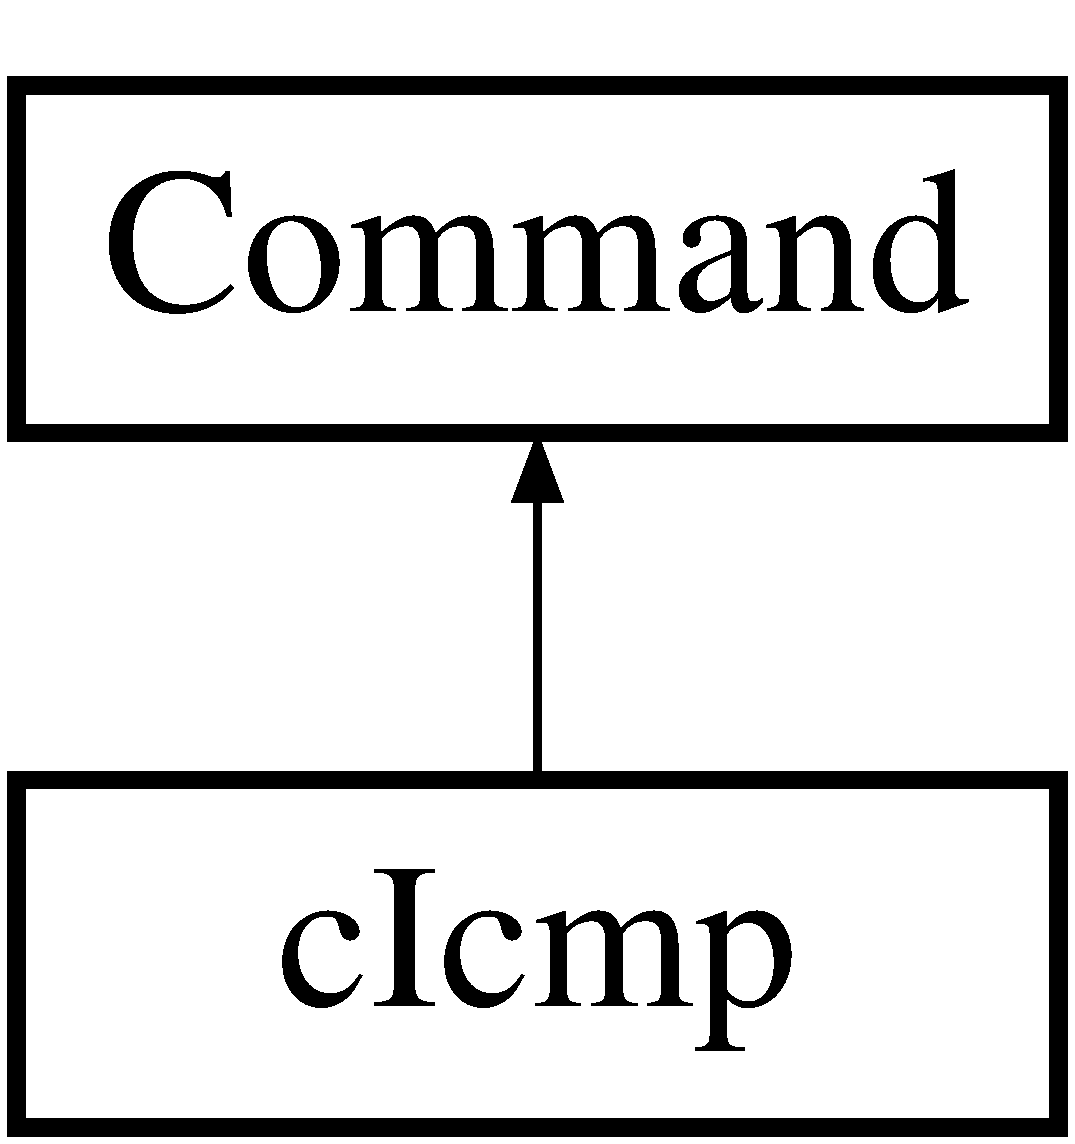
\includegraphics[height=2.000000cm]{classc_icmp}
\end{center}
\end{figure}
\subsection*{Открытые члены}
\begin{DoxyCompactItemize}
\item 
int \hyperlink{classc_icmp_abde58eb4e568e089f38966a4c6ab6256}{operator()} (\hyperlink{class_computer}{Computer} $\ast$C\+O\+MP)
\begin{DoxyCompactList}\small\item\em c\+Icmp\+::operator () -\/ Сравнение целых чисел \end{DoxyCompactList}\end{DoxyCompactItemize}
\subsection*{Дополнительные унаследованные члены}


\subsection{Подробное описание}
Сравнение целых 

\subsection{Методы}
\hypertarget{classc_icmp_abde58eb4e568e089f38966a4c6ab6256}{}\label{classc_icmp_abde58eb4e568e089f38966a4c6ab6256} 
\index{c\+Icmp@{c\+Icmp}!operator()@{operator()}}
\index{operator()@{operator()}!c\+Icmp@{c\+Icmp}}
\subsubsection{\texorpdfstring{operator()()}{operator()()}}
{\footnotesize\ttfamily int c\+Icmp\+::operator() (\begin{DoxyParamCaption}\item[{\hyperlink{class_computer}{Computer} $\ast$}]{C\+O\+MP }\end{DoxyParamCaption})\hspace{0.3cm}{\ttfamily [virtual]}}



c\+Icmp\+::operator () -\/ Сравнение целых чисел 


\begin{DoxyParams}{Аргументы}
{\em C\+O\+MP} & -\/ указатель на объект компьютер \\
\hline
\end{DoxyParams}
\begin{DoxyReturn}{Возвращает}
1
\end{DoxyReturn}
Загружает внутренний регистр из памяти. Сравнивает целочисленное значение сумматора с целочисленныйм значением внутреннего регистра. Результаты записываются в флаги P\+SW. Значение сумматора не изменяется. 

Замещает \hyperlink{class_command_a79939b66f3de892e91d7710844294716}{Command}.


\begin{DoxyCode}
290 \{
291     \hyperlink{class_command_aac6f368e7c9dbb357b3f00627d5dabfc}{loadRegister}(COMP);
292     COMP->\hyperlink{class_computer_adb154047da2156e4419af3b3a4a766b7}{DATA}.\hyperlink{union_computer_1_1data_a6e51de6e0351adc4e50b336a092bc4bb}{I} = COMP->\hyperlink{class_computer_a874503110664b3cf821118d2ce9c2b96}{RS}.\hyperlink{union_computer_1_1data_a6e51de6e0351adc4e50b336a092bc4bb}{I};
293     COMP->\hyperlink{class_computer_a874503110664b3cf821118d2ce9c2b96}{RS}.\hyperlink{union_computer_1_1data_a6e51de6e0351adc4e50b336a092bc4bb}{I} -= COMP->\hyperlink{class_computer_a0fbf84599b7db9d634a92afed443ee73}{R1}.\hyperlink{union_computer_1_1data_a6e51de6e0351adc4e50b336a092bc4bb}{I};
294     COMP->\hyperlink{class_computer_aae4a76a8a03a6c9fb1c12968d629be3e}{flagI}(); \textcolor{comment}{//Установка флага результата}
295     COMP->\hyperlink{class_computer_a874503110664b3cf821118d2ce9c2b96}{RS}.\hyperlink{union_computer_1_1data_a6e51de6e0351adc4e50b336a092bc4bb}{I} = COMP->\hyperlink{class_computer_adb154047da2156e4419af3b3a4a766b7}{DATA}.\hyperlink{union_computer_1_1data_a6e51de6e0351adc4e50b336a092bc4bb}{I};
296 
297     COMP->\hyperlink{class_computer_a10ca6c6b200630119201de16d7368e0f}{debug}(\textcolor{stringliteral}{"Целочисленное сравнение"});
298     \textcolor{keywordflow}{return} 1;
299 \}
\end{DoxyCode}


Объявления и описания членов классов находятся в файлах\+:\begin{DoxyCompactItemize}
\item 
C\+:/\+Users/sstarkov/\+Documents/kr\+\_\+\+Interpreter\+V\+M/sources/command.\+h\item 
C\+:/\+Users/sstarkov/\+Documents/kr\+\_\+\+Interpreter\+V\+M/sources/command.\+cpp\end{DoxyCompactItemize}

\hypertarget{classc_idiv}{}\section{Класс c\+Idiv}
\label{classc_idiv}\index{c\+Idiv@{c\+Idiv}}


Деление целых чисел  




{\ttfamily \#include $<$command.\+h$>$}

Граф наследования\+:c\+Idiv\+:\begin{figure}[H]
\begin{center}
\leavevmode
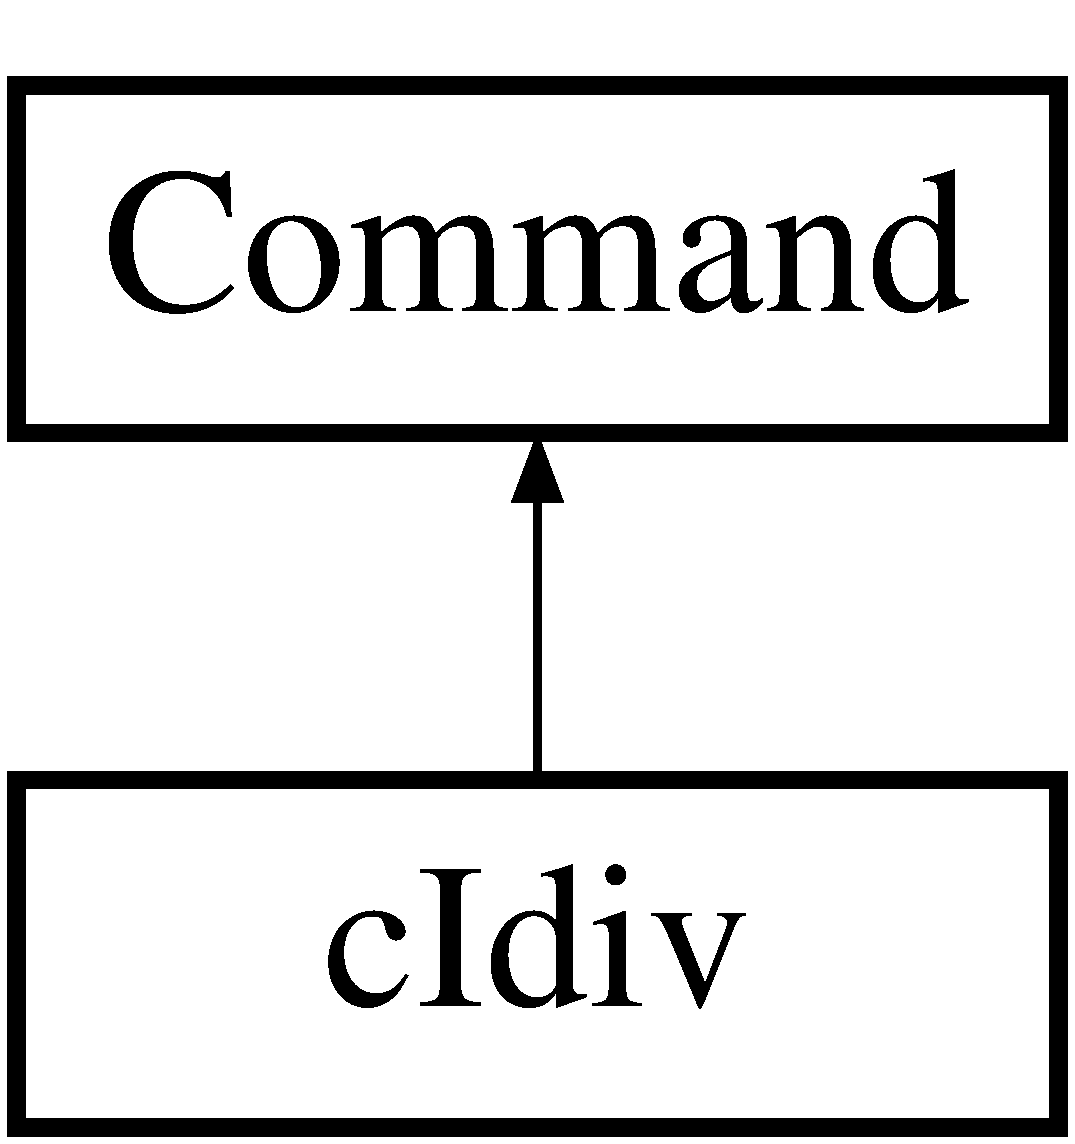
\includegraphics[height=2.000000cm]{classc_idiv}
\end{center}
\end{figure}
\subsection*{Открытые члены}
\begin{DoxyCompactItemize}
\item 
int \hyperlink{classc_idiv_ae7b137fbea1950b954729c2040be22d5}{operator()} (\hyperlink{class_computer}{Computer} $\ast$C\+O\+MP)
\begin{DoxyCompactList}\small\item\em c\+Idiv\+::operator () -\/ Целочисленное деление \end{DoxyCompactList}\end{DoxyCompactItemize}
\subsection*{Дополнительные унаследованные члены}


\subsection{Подробное описание}
Деление целых чисел 

\subsection{Методы}
\hypertarget{classc_idiv_ae7b137fbea1950b954729c2040be22d5}{}\label{classc_idiv_ae7b137fbea1950b954729c2040be22d5} 
\index{c\+Idiv@{c\+Idiv}!operator()@{operator()}}
\index{operator()@{operator()}!c\+Idiv@{c\+Idiv}}
\subsubsection{\texorpdfstring{operator()()}{operator()()}}
{\footnotesize\ttfamily int c\+Idiv\+::operator() (\begin{DoxyParamCaption}\item[{\hyperlink{class_computer}{Computer} $\ast$}]{C\+O\+MP }\end{DoxyParamCaption})\hspace{0.3cm}{\ttfamily [virtual]}}



c\+Idiv\+::operator () -\/ Целочисленное деление 


\begin{DoxyParams}{Аргументы}
{\em C\+O\+MP} & -\/ указатель на объект компьютер \\
\hline
\end{DoxyParams}
\begin{DoxyReturn}{Возвращает}
1
\end{DoxyReturn}
Загружает внутренний регистр по адресу. Делит сумматор на значение внутреннего регистра. Ставит флаги операции. 

Замещает \hyperlink{class_command_a79939b66f3de892e91d7710844294716}{Command}.


\begin{DoxyCode}
104 \{
105     \hyperlink{class_command_aac6f368e7c9dbb357b3f00627d5dabfc}{loadRegister}(COMP);
106     COMP->\hyperlink{class_computer_a874503110664b3cf821118d2ce9c2b96}{RS}.\hyperlink{union_computer_1_1data_a6e51de6e0351adc4e50b336a092bc4bb}{I} /= COMP->\hyperlink{class_computer_a0fbf84599b7db9d634a92afed443ee73}{R1}.\hyperlink{union_computer_1_1data_a6e51de6e0351adc4e50b336a092bc4bb}{I};
107     COMP->\hyperlink{class_computer_aae4a76a8a03a6c9fb1c12968d629be3e}{flagI}(); \textcolor{comment}{//Установка флага результата}
108 
109     COMP->\hyperlink{class_computer_a10ca6c6b200630119201de16d7368e0f}{debug}(\textcolor{stringliteral}{"Целочисленное деление. Сумматор = "} + QString::number(COMP->
      \hyperlink{class_computer_a874503110664b3cf821118d2ce9c2b96}{RS}.\hyperlink{union_computer_1_1data_a6e51de6e0351adc4e50b336a092bc4bb}{I}));
110     \textcolor{keywordflow}{return} 1;
111 \}
\end{DoxyCode}


Объявления и описания членов классов находятся в файлах\+:\begin{DoxyCompactItemize}
\item 
C\+:/\+Users/sstarkov/\+Documents/kr\+\_\+\+Interpreter\+V\+M/sources/command.\+h\item 
C\+:/\+Users/sstarkov/\+Documents/kr\+\_\+\+Interpreter\+V\+M/sources/command.\+cpp\end{DoxyCompactItemize}

\hypertarget{classc_iin}{}\section{Класс c\+Iin}
\label{classc_iin}\index{c\+Iin@{c\+Iin}}


Ввод целого  




{\ttfamily \#include $<$command.\+h$>$}

Граф наследования\+:c\+Iin\+:\begin{figure}[H]
\begin{center}
\leavevmode
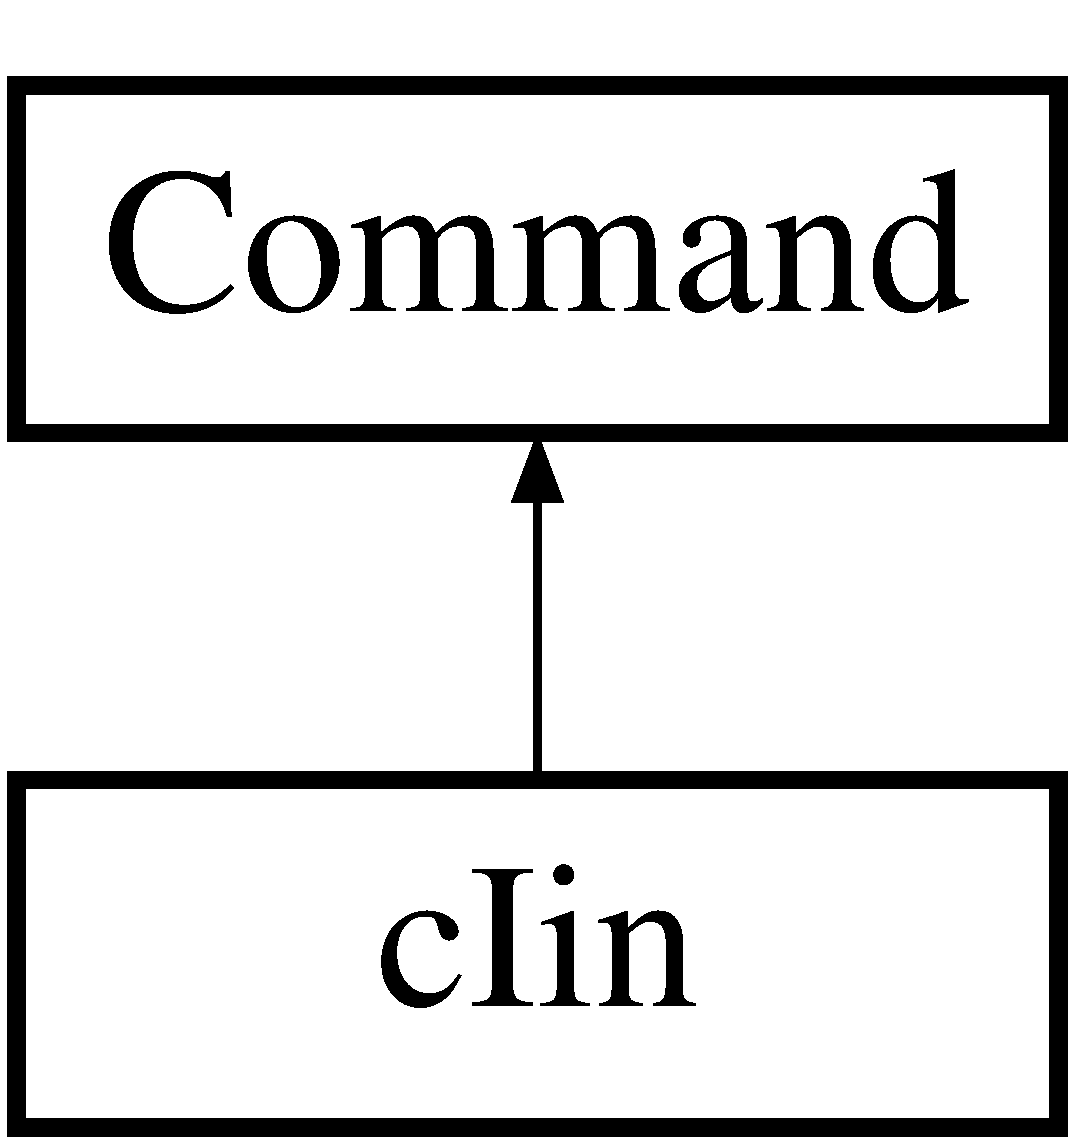
\includegraphics[height=2.000000cm]{classc_iin}
\end{center}
\end{figure}
\subsection*{Открытые члены}
\begin{DoxyCompactItemize}
\item 
int \hyperlink{classc_iin_a80d23ca91e78c52713f1d645df0d1d7d}{operator()} (\hyperlink{class_computer}{Computer} $\ast$C\+O\+MP)
\begin{DoxyCompactList}\small\item\em c\+Iin\+::operator () -\/ Прерывание\+: ввод вещественного значения \end{DoxyCompactList}\end{DoxyCompactItemize}
\subsection*{Дополнительные унаследованные члены}


\subsection{Подробное описание}
Ввод целого 

\subsection{Методы}
\hypertarget{classc_iin_a80d23ca91e78c52713f1d645df0d1d7d}{}\label{classc_iin_a80d23ca91e78c52713f1d645df0d1d7d} 
\index{c\+Iin@{c\+Iin}!operator()@{operator()}}
\index{operator()@{operator()}!c\+Iin@{c\+Iin}}
\subsubsection{\texorpdfstring{operator()()}{operator()()}}
{\footnotesize\ttfamily int c\+Iin\+::operator() (\begin{DoxyParamCaption}\item[{\hyperlink{class_computer}{Computer} $\ast$}]{C\+O\+MP }\end{DoxyParamCaption})\hspace{0.3cm}{\ttfamily [virtual]}}



c\+Iin\+::operator () -\/ Прерывание\+: ввод вещественного значения 


\begin{DoxyParams}{Аргументы}
{\em C\+O\+MP} & -\/ указатель на объект компьютер \\
\hline
\end{DoxyParams}
\begin{DoxyReturn}{Возвращает}
1
\end{DoxyReturn}
Вызывает прерывание для ввода целочисленного значения от пользователя и загружает его в сумматор 

Замещает \hyperlink{class_command_a79939b66f3de892e91d7710844294716}{Command}.


\begin{DoxyCode}
409 \{
410     COMP->\hyperlink{class_computer_aa57b0ed2f3a9b168c2924174ec524bd4}{interrupt}(hIin);
411     COMP->\hyperlink{class_computer_a874503110664b3cf821118d2ce9c2b96}{RS}.\hyperlink{union_computer_1_1data_a6e51de6e0351adc4e50b336a092bc4bb}{I} = COMP->\hyperlink{class_computer_adb154047da2156e4419af3b3a4a766b7}{DATA}.\hyperlink{union_computer_1_1data_a6e51de6e0351adc4e50b336a092bc4bb}{I};
412 
413     COMP->\hyperlink{class_computer_a10ca6c6b200630119201de16d7368e0f}{debug}(\textcolor{stringliteral}{"Ввод целого числа "} + QString::number(COMP->\hyperlink{class_computer_a874503110664b3cf821118d2ce9c2b96}{RS}.\hyperlink{union_computer_1_1data_a6e51de6e0351adc4e50b336a092bc4bb}{I}));
414     \textcolor{keywordflow}{return} 1;
415 \}
\end{DoxyCode}


Объявления и описания членов классов находятся в файлах\+:\begin{DoxyCompactItemize}
\item 
C\+:/\+Users/sstarkov/\+Documents/kr\+\_\+\+Interpreter\+V\+M/sources/command.\+h\item 
C\+:/\+Users/sstarkov/\+Documents/kr\+\_\+\+Interpreter\+V\+M/sources/command.\+cpp\end{DoxyCompactItemize}

\hypertarget{classc_imod}{}\section{Класс c\+Imod}
\label{classc_imod}\index{c\+Imod@{c\+Imod}}


Остаток от деления целых чисел  




{\ttfamily \#include $<$command.\+h$>$}

Граф наследования\+:c\+Imod\+:\begin{figure}[H]
\begin{center}
\leavevmode
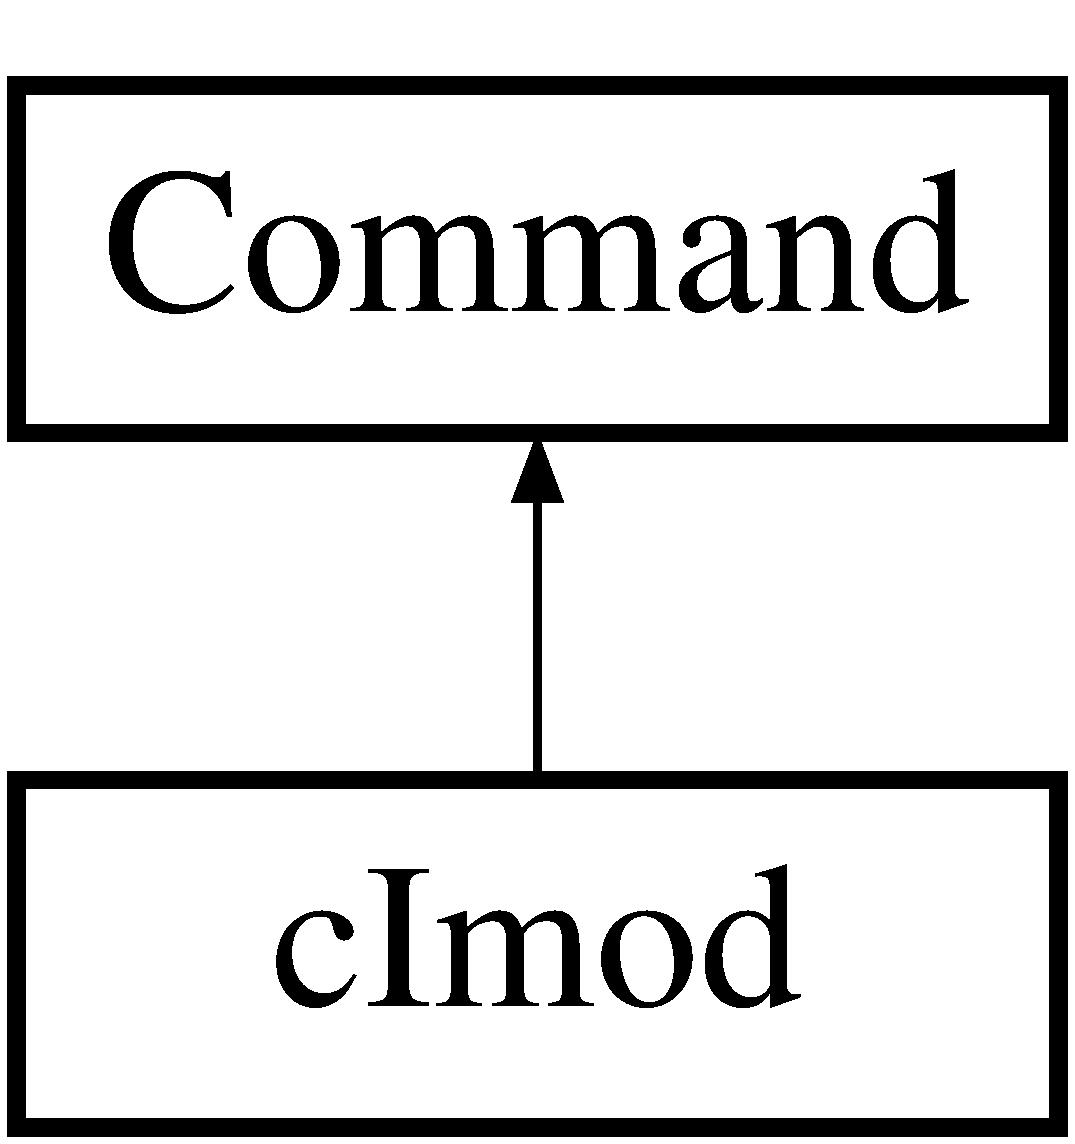
\includegraphics[height=2.000000cm]{classc_imod}
\end{center}
\end{figure}
\subsection*{Открытые члены}
\begin{DoxyCompactItemize}
\item 
int \hyperlink{classc_imod_a2a46c860bd31b90c26081e8e450532e5}{operator()} (\hyperlink{class_computer}{Computer} $\ast$C\+O\+MP)
\begin{DoxyCompactList}\small\item\em c\+Imod\+::operator () -\/ Целочисленный остаток от деления \end{DoxyCompactList}\end{DoxyCompactItemize}
\subsection*{Дополнительные унаследованные члены}


\subsection{Подробное описание}
Остаток от деления целых чисел 

\subsection{Методы}
\hypertarget{classc_imod_a2a46c860bd31b90c26081e8e450532e5}{}\label{classc_imod_a2a46c860bd31b90c26081e8e450532e5} 
\index{c\+Imod@{c\+Imod}!operator()@{operator()}}
\index{operator()@{operator()}!c\+Imod@{c\+Imod}}
\subsubsection{\texorpdfstring{operator()()}{operator()()}}
{\footnotesize\ttfamily int c\+Imod\+::operator() (\begin{DoxyParamCaption}\item[{\hyperlink{class_computer}{Computer} $\ast$}]{C\+O\+MP }\end{DoxyParamCaption})\hspace{0.3cm}{\ttfamily [virtual]}}



c\+Imod\+::operator () -\/ Целочисленный остаток от деления 


\begin{DoxyParams}{Аргументы}
{\em C\+O\+MP} & -\/ указатель на объект компьютер \\
\hline
\end{DoxyParams}
\begin{DoxyReturn}{Возвращает}
1
\end{DoxyReturn}
Загружает внутренний регистр по адресу. Записывает в сумматор остаток от деления сумматоран на значение внутреннего регистра. Ставит флаги операции. 

Замещает \hyperlink{class_command_a79939b66f3de892e91d7710844294716}{Command}.


\begin{DoxyCode}
123 \{
124     \hyperlink{class_command_aac6f368e7c9dbb357b3f00627d5dabfc}{loadRegister}(COMP);
125     COMP->\hyperlink{class_computer_a874503110664b3cf821118d2ce9c2b96}{RS}.\hyperlink{union_computer_1_1data_a6e51de6e0351adc4e50b336a092bc4bb}{I} %= COMP->\hyperlink{class_computer_a0fbf84599b7db9d634a92afed443ee73}{R1}.\hyperlink{union_computer_1_1data_a6e51de6e0351adc4e50b336a092bc4bb}{I};
126     COMP->\hyperlink{class_computer_aae4a76a8a03a6c9fb1c12968d629be3e}{flagI}(); \textcolor{comment}{//Установка флага результата}
127 
128     COMP->\hyperlink{class_computer_a10ca6c6b200630119201de16d7368e0f}{debug}(\textcolor{stringliteral}{"Целочисленный остаток от деления. Сумматор = "} + QString::number(COMP->
      \hyperlink{class_computer_a874503110664b3cf821118d2ce9c2b96}{RS}.\hyperlink{union_computer_1_1data_a6e51de6e0351adc4e50b336a092bc4bb}{I}));
129     \textcolor{keywordflow}{return} 1;
130 \}
\end{DoxyCode}


Объявления и описания членов классов находятся в файлах\+:\begin{DoxyCompactItemize}
\item 
C\+:/\+Users/sstarkov/\+Documents/kr\+\_\+\+Interpreter\+V\+M/sources/command.\+h\item 
C\+:/\+Users/sstarkov/\+Documents/kr\+\_\+\+Interpreter\+V\+M/sources/command.\+cpp\end{DoxyCompactItemize}

\hypertarget{classc_imul}{}\section{Класс c\+Imul}
\label{classc_imul}\index{c\+Imul@{c\+Imul}}


Умножение целых чисел  




{\ttfamily \#include $<$command.\+h$>$}

Граф наследования\+:c\+Imul\+:\begin{figure}[H]
\begin{center}
\leavevmode
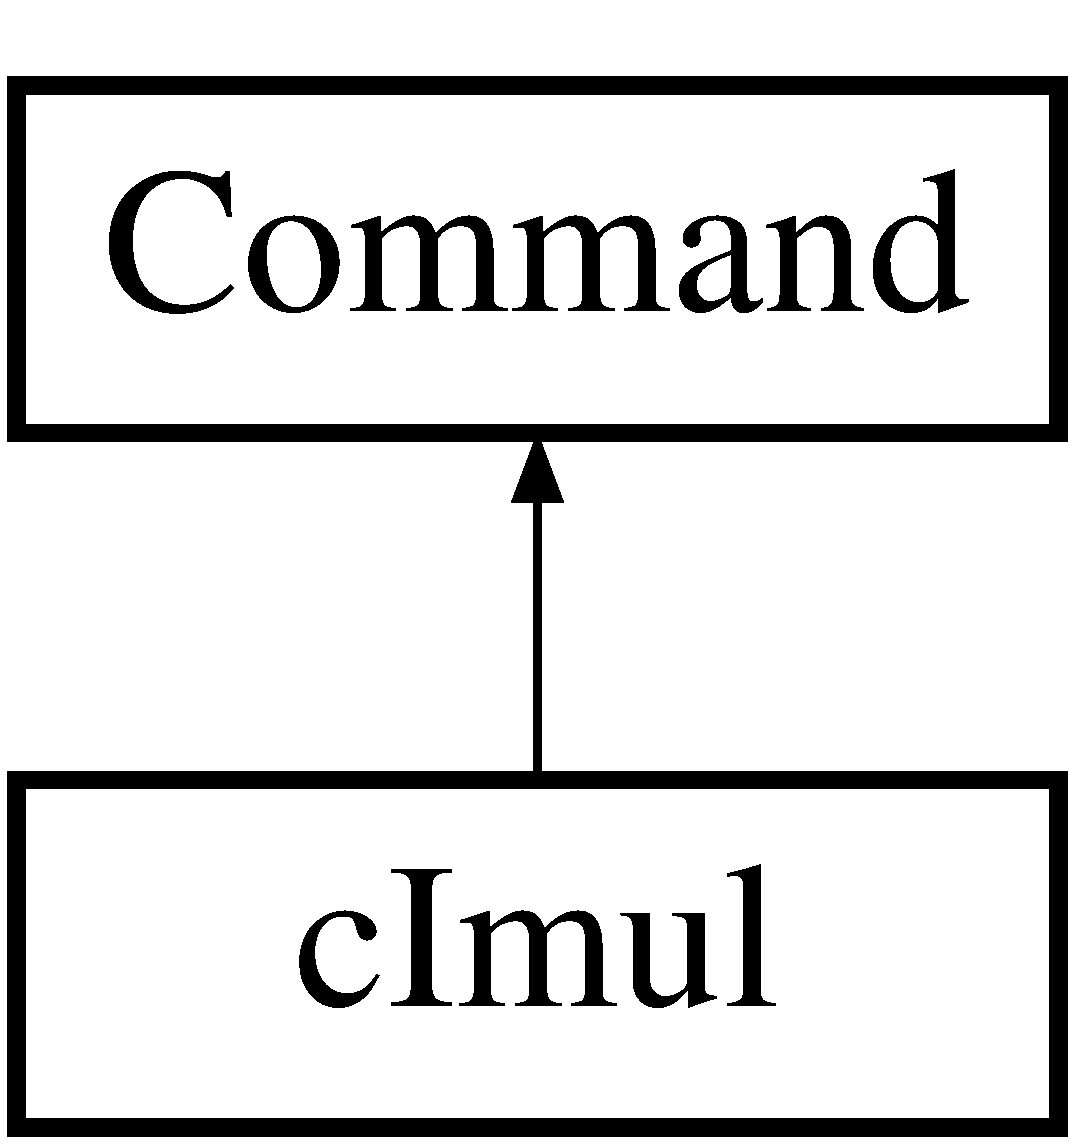
\includegraphics[height=2.000000cm]{classc_imul}
\end{center}
\end{figure}
\subsection*{Открытые члены}
\begin{DoxyCompactItemize}
\item 
int \hyperlink{classc_imul_a2bdd2bb819f2a86d34de28a4c0764398}{operator()} (\hyperlink{class_computer}{Computer} $\ast$C\+O\+MP)
\begin{DoxyCompactList}\small\item\em c\+Imul\+::operator () -\/ Целочисленное произведение \end{DoxyCompactList}\end{DoxyCompactItemize}
\subsection*{Дополнительные унаследованные члены}


\subsection{Подробное описание}
Умножение целых чисел 

\subsection{Методы}
\hypertarget{classc_imul_a2bdd2bb819f2a86d34de28a4c0764398}{}\label{classc_imul_a2bdd2bb819f2a86d34de28a4c0764398} 
\index{c\+Imul@{c\+Imul}!operator()@{operator()}}
\index{operator()@{operator()}!c\+Imul@{c\+Imul}}
\subsubsection{\texorpdfstring{operator()()}{operator()()}}
{\footnotesize\ttfamily int c\+Imul\+::operator() (\begin{DoxyParamCaption}\item[{\hyperlink{class_computer}{Computer} $\ast$}]{C\+O\+MP }\end{DoxyParamCaption})\hspace{0.3cm}{\ttfamily [virtual]}}



c\+Imul\+::operator () -\/ Целочисленное произведение 


\begin{DoxyParams}{Аргументы}
{\em C\+O\+MP} & -\/ указатель на объект компьютер \\
\hline
\end{DoxyParams}
\begin{DoxyReturn}{Возвращает}
1
\end{DoxyReturn}
Загружает внутренний регистр по адресу. Умножает сумматор на внутренний регистр Ставит флаги операции. 

Замещает \hyperlink{class_command_a79939b66f3de892e91d7710844294716}{Command}.


\begin{DoxyCode}
85 \{
86     \hyperlink{class_command_aac6f368e7c9dbb357b3f00627d5dabfc}{loadRegister}(COMP);
87     COMP->\hyperlink{class_computer_a874503110664b3cf821118d2ce9c2b96}{RS}.\hyperlink{union_computer_1_1data_a6e51de6e0351adc4e50b336a092bc4bb}{I} *= COMP->\hyperlink{class_computer_a0fbf84599b7db9d634a92afed443ee73}{R1}.\hyperlink{union_computer_1_1data_a6e51de6e0351adc4e50b336a092bc4bb}{I};
88     COMP->\hyperlink{class_computer_aae4a76a8a03a6c9fb1c12968d629be3e}{flagI}(); \textcolor{comment}{//Установка флага результата}
89 
90     COMP->\hyperlink{class_computer_a10ca6c6b200630119201de16d7368e0f}{debug}(\textcolor{stringliteral}{"Целочисленное умножение. Сумматор = "} + QString::number(COMP->
      \hyperlink{class_computer_a874503110664b3cf821118d2ce9c2b96}{RS}.\hyperlink{union_computer_1_1data_a6e51de6e0351adc4e50b336a092bc4bb}{I}));
91     \textcolor{keywordflow}{return} 1;
92 \}
\end{DoxyCode}


Объявления и описания членов классов находятся в файлах\+:\begin{DoxyCompactItemize}
\item 
C\+:/\+Users/sstarkov/\+Documents/kr\+\_\+\+Interpreter\+V\+M/sources/command.\+h\item 
C\+:/\+Users/sstarkov/\+Documents/kr\+\_\+\+Interpreter\+V\+M/sources/command.\+cpp\end{DoxyCompactItemize}

\hypertarget{classc_iout}{}\section{Класс c\+Iout}
\label{classc_iout}\index{c\+Iout@{c\+Iout}}


вывод целого  




{\ttfamily \#include $<$command.\+h$>$}

Граф наследования\+:c\+Iout\+:\begin{figure}[H]
\begin{center}
\leavevmode
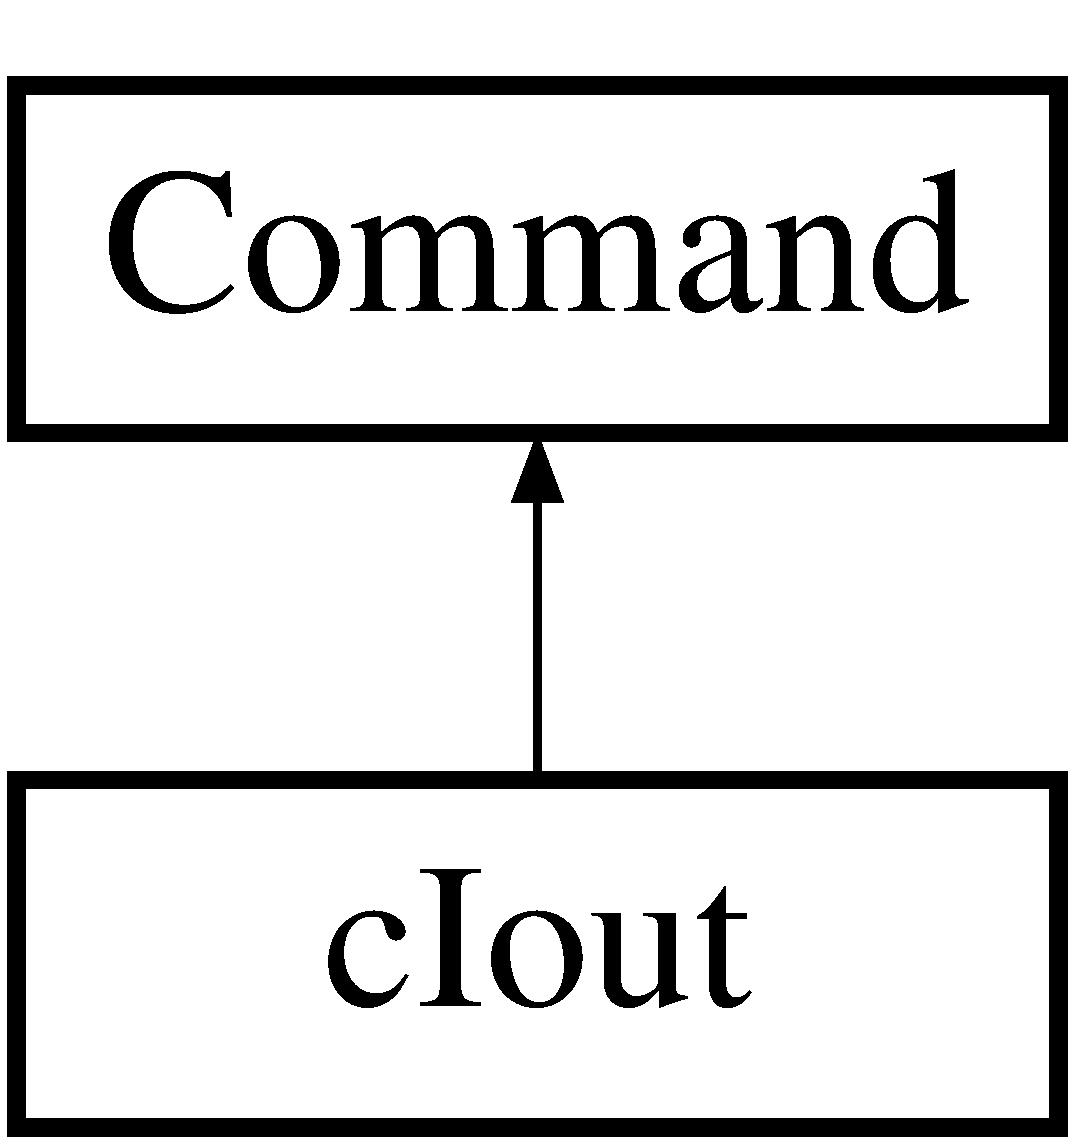
\includegraphics[height=2.000000cm]{classc_iout}
\end{center}
\end{figure}
\subsection*{Открытые члены}
\begin{DoxyCompactItemize}
\item 
int \hyperlink{classc_iout_a82536616889a02f99211d79920bad3dd}{operator()} (\hyperlink{class_computer}{Computer} $\ast$C\+O\+MP)
\begin{DoxyCompactList}\small\item\em c\+Iout\+::operator () -\/ Прерывание\+: вывод целого значения \end{DoxyCompactList}\end{DoxyCompactItemize}
\subsection*{Дополнительные унаследованные члены}


\subsection{Подробное описание}
вывод целого 

\subsection{Методы}
\hypertarget{classc_iout_a82536616889a02f99211d79920bad3dd}{}\label{classc_iout_a82536616889a02f99211d79920bad3dd} 
\index{c\+Iout@{c\+Iout}!operator()@{operator()}}
\index{operator()@{operator()}!c\+Iout@{c\+Iout}}
\subsubsection{\texorpdfstring{operator()()}{operator()()}}
{\footnotesize\ttfamily int c\+Iout\+::operator() (\begin{DoxyParamCaption}\item[{\hyperlink{class_computer}{Computer} $\ast$}]{C\+O\+MP }\end{DoxyParamCaption})\hspace{0.3cm}{\ttfamily [virtual]}}



c\+Iout\+::operator () -\/ Прерывание\+: вывод целого значения 


\begin{DoxyParams}{Аргументы}
{\em C\+O\+MP} & -\/ указатель на объект компьютер \\
\hline
\end{DoxyParams}
\begin{DoxyReturn}{Возвращает}
1
\end{DoxyReturn}
Вызывает прерывание для вывода целочисленного значения на экран из сумматора 

Замещает \hyperlink{class_command_a79939b66f3de892e91d7710844294716}{Command}.


\begin{DoxyCode}
441 \{
442     COMP->\hyperlink{class_computer_a10ca6c6b200630119201de16d7368e0f}{debug}(\textcolor{stringliteral}{"Вывод целого числа "} + QString::number(COMP->\hyperlink{class_computer_a874503110664b3cf821118d2ce9c2b96}{RS}.\hyperlink{union_computer_1_1data_a6e51de6e0351adc4e50b336a092bc4bb}{I}));
443     COMP->\hyperlink{class_computer_aa57b0ed2f3a9b168c2924174ec524bd4}{interrupt}(hIout);
444     \textcolor{keywordflow}{return} 1;
445 \}
\end{DoxyCode}


Объявления и описания членов классов находятся в файлах\+:\begin{DoxyCompactItemize}
\item 
C\+:/\+Users/sstarkov/\+Documents/kr\+\_\+\+Interpreter\+V\+M/sources/command.\+h\item 
C\+:/\+Users/sstarkov/\+Documents/kr\+\_\+\+Interpreter\+V\+M/sources/command.\+cpp\end{DoxyCompactItemize}

\hypertarget{classc_isub}{}\section{Класс c\+Isub}
\label{classc_isub}\index{c\+Isub@{c\+Isub}}


Вычитание целых чисел  




{\ttfamily \#include $<$command.\+h$>$}

Граф наследования\+:c\+Isub\+:\begin{figure}[H]
\begin{center}
\leavevmode
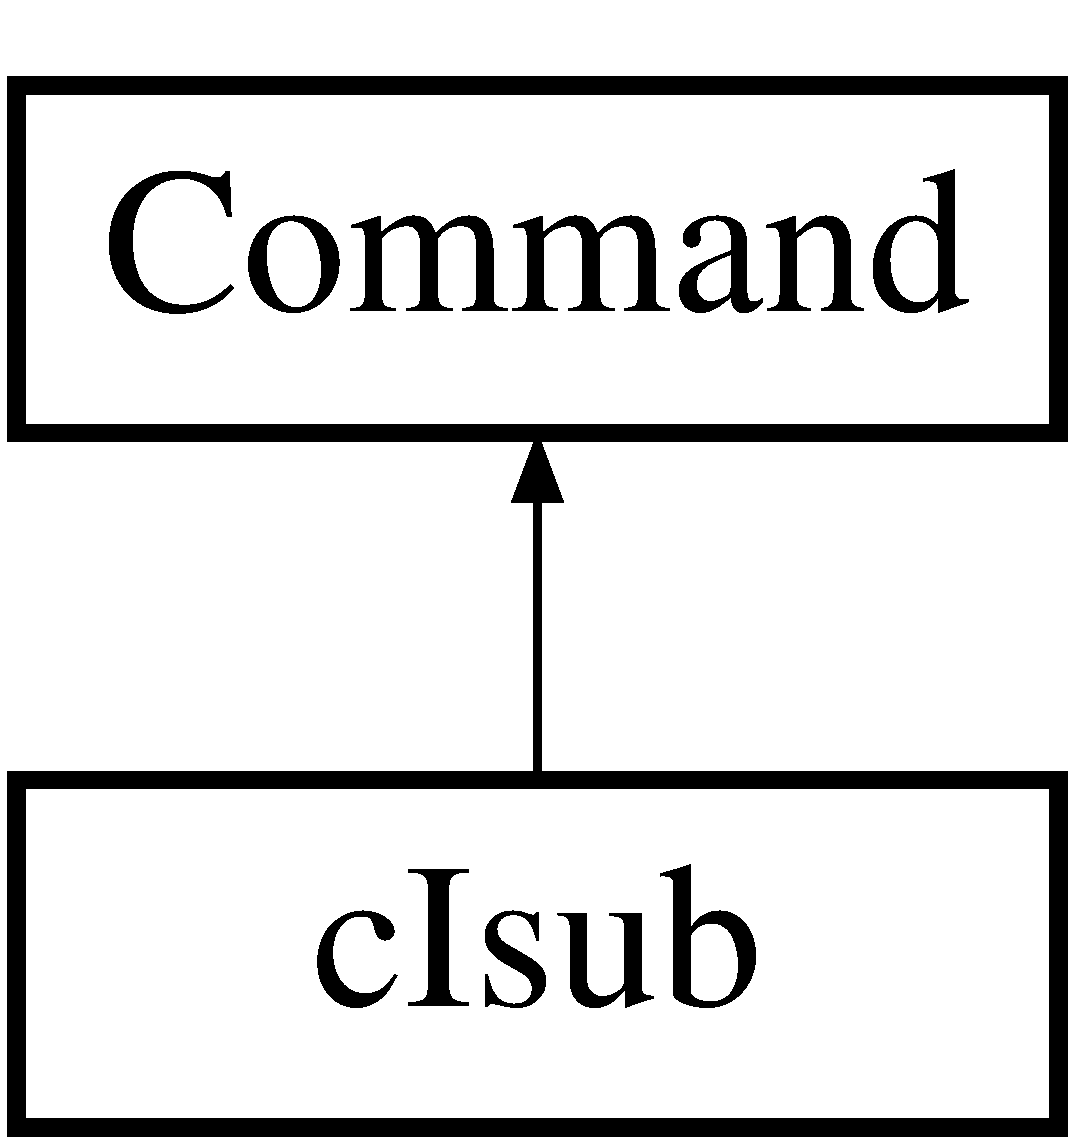
\includegraphics[height=2.000000cm]{classc_isub}
\end{center}
\end{figure}
\subsection*{Открытые члены}
\begin{DoxyCompactItemize}
\item 
int \hyperlink{classc_isub_ab4f6204ec8c69ce3342228c52fd30a05}{operator()} (\hyperlink{class_computer}{Computer} $\ast$C\+O\+MP)
\begin{DoxyCompactList}\small\item\em c\+Isub\+::operator () -\/ Целочисленная разность \end{DoxyCompactList}\end{DoxyCompactItemize}
\subsection*{Дополнительные унаследованные члены}


\subsection{Подробное описание}
Вычитание целых чисел 

\subsection{Методы}
\hypertarget{classc_isub_ab4f6204ec8c69ce3342228c52fd30a05}{}\label{classc_isub_ab4f6204ec8c69ce3342228c52fd30a05} 
\index{c\+Isub@{c\+Isub}!operator()@{operator()}}
\index{operator()@{operator()}!c\+Isub@{c\+Isub}}
\subsubsection{\texorpdfstring{operator()()}{operator()()}}
{\footnotesize\ttfamily int c\+Isub\+::operator() (\begin{DoxyParamCaption}\item[{\hyperlink{class_computer}{Computer} $\ast$}]{C\+O\+MP }\end{DoxyParamCaption})\hspace{0.3cm}{\ttfamily [virtual]}}



c\+Isub\+::operator () -\/ Целочисленная разность 


\begin{DoxyParams}{Аргументы}
{\em C\+O\+MP} & -\/ указатель на объект компьютер \\
\hline
\end{DoxyParams}
\begin{DoxyReturn}{Возвращает}
1
\end{DoxyReturn}
Загружает внутренний регистр по адресу. Вичитает из сумматора значение внутреннего регистра. Ставит флаги операции. 

Замещает \hyperlink{class_command_a79939b66f3de892e91d7710844294716}{Command}.


\begin{DoxyCode}
66 \{
67     \hyperlink{class_command_aac6f368e7c9dbb357b3f00627d5dabfc}{loadRegister}(COMP);
68     COMP->\hyperlink{class_computer_a874503110664b3cf821118d2ce9c2b96}{RS}.\hyperlink{union_computer_1_1data_a6e51de6e0351adc4e50b336a092bc4bb}{I} -= COMP->\hyperlink{class_computer_a0fbf84599b7db9d634a92afed443ee73}{R1}.\hyperlink{union_computer_1_1data_a6e51de6e0351adc4e50b336a092bc4bb}{I};
69     COMP->\hyperlink{class_computer_aae4a76a8a03a6c9fb1c12968d629be3e}{flagI}(); \textcolor{comment}{//Установка флага результата}
70 
71     COMP->\hyperlink{class_computer_a10ca6c6b200630119201de16d7368e0f}{debug}(\textcolor{stringliteral}{"Целочисленное вычитание. Сумматор = "} + QString::number(COMP->
      \hyperlink{class_computer_a874503110664b3cf821118d2ce9c2b96}{RS}.\hyperlink{union_computer_1_1data_a6e51de6e0351adc4e50b336a092bc4bb}{I}));
72     \textcolor{keywordflow}{return} 1;
73 \}
\end{DoxyCode}


Объявления и описания членов классов находятся в файлах\+:\begin{DoxyCompactItemize}
\item 
C\+:/\+Users/sstarkov/\+Documents/kr\+\_\+\+Interpreter\+V\+M/sources/command.\+h\item 
C\+:/\+Users/sstarkov/\+Documents/kr\+\_\+\+Interpreter\+V\+M/sources/command.\+cpp\end{DoxyCompactItemize}

\hypertarget{classc_j_g}{}\section{Класс c\+JG}
\label{classc_j_g}\index{c\+JG@{c\+JG}}


переход, если больше  




{\ttfamily \#include $<$command.\+h$>$}

Граф наследования\+:c\+JG\+:\begin{figure}[H]
\begin{center}
\leavevmode
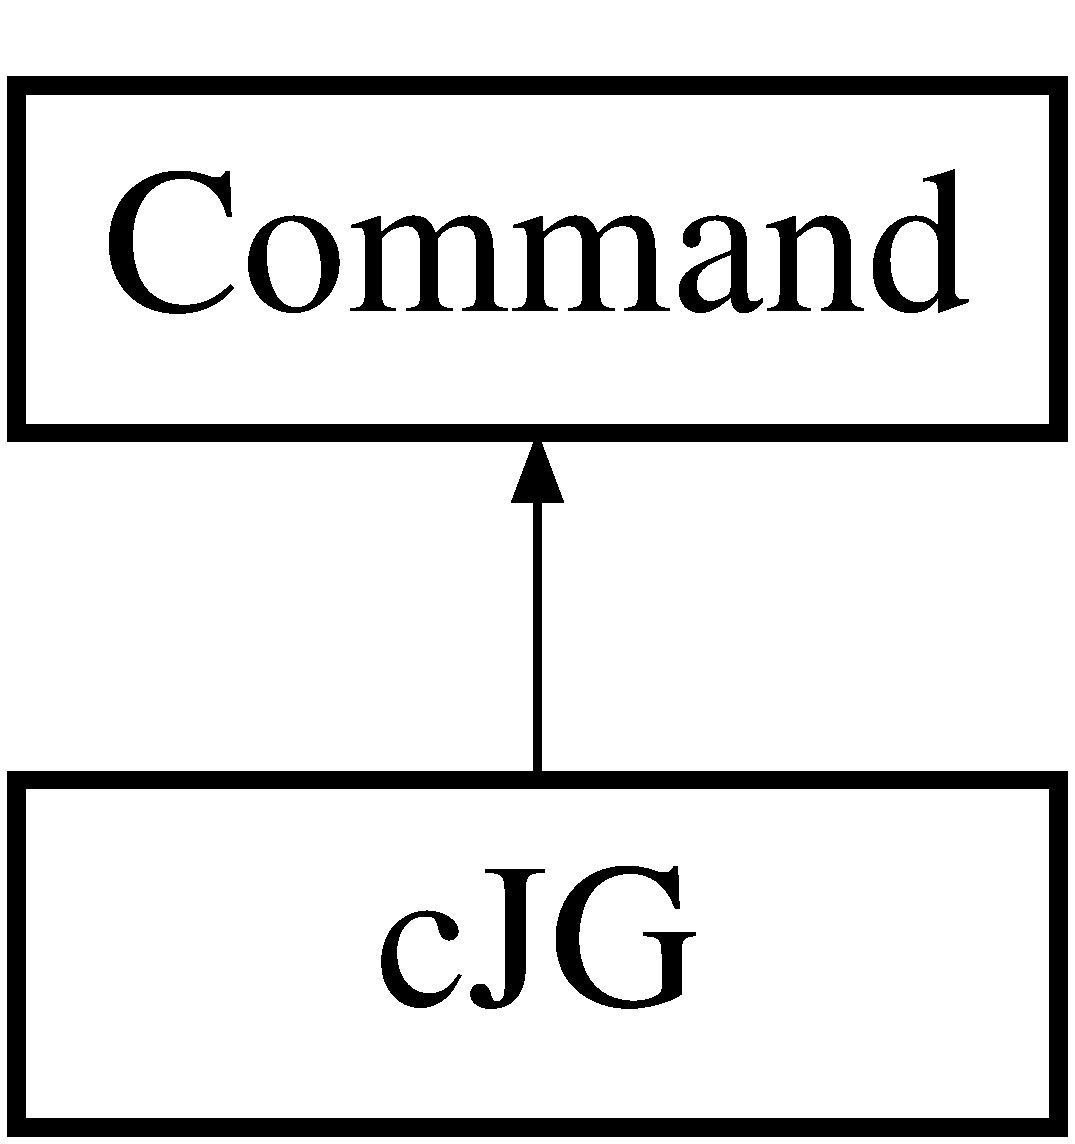
\includegraphics[height=2.000000cm]{classc_j_g}
\end{center}
\end{figure}
\subsection*{Открытые члены}
\begin{DoxyCompactItemize}
\item 
int \hyperlink{classc_j_g_a3e2f3b6fc18af11c937a81e83b065ede}{operator()} (\hyperlink{class_computer}{Computer} $\ast$C\+O\+MP)
\begin{DoxyCompactList}\small\item\em c\+J\+G\+::operator () -\/ Переход если больше \end{DoxyCompactList}\end{DoxyCompactItemize}
\subsection*{Дополнительные унаследованные члены}


\subsection{Подробное описание}
переход, если больше 

\subsection{Методы}
\hypertarget{classc_j_g_a3e2f3b6fc18af11c937a81e83b065ede}{}\label{classc_j_g_a3e2f3b6fc18af11c937a81e83b065ede} 
\index{c\+JG@{c\+JG}!operator()@{operator()}}
\index{operator()@{operator()}!c\+JG@{c\+JG}}
\subsubsection{\texorpdfstring{operator()()}{operator()()}}
{\footnotesize\ttfamily int c\+J\+G\+::operator() (\begin{DoxyParamCaption}\item[{\hyperlink{class_computer}{Computer} $\ast$}]{C\+O\+MP }\end{DoxyParamCaption})\hspace{0.3cm}{\ttfamily [virtual]}}



c\+J\+G\+::operator () -\/ Переход если больше 


\begin{DoxyParams}{Аргументы}
{\em C\+O\+MP} & -\/ указатель на объект компьютер \\
\hline
\end{DoxyParams}
\begin{DoxyReturn}{Возвращает}
1
\end{DoxyReturn}
Если по результатам сравнения Icmp или Rcmp сумматор был больше адресного регистра, изменяет значение указателя на инструкцию по абсолютному значению адреса ОЗУ, либо отступа от текущего значения. 

Замещает \hyperlink{class_command_a79939b66f3de892e91d7710844294716}{Command}.


\begin{DoxyCode}
370 \{
371     \textcolor{keywordflow}{if}(COMP->\hyperlink{class_computer_aada011a29d87bb979835371a5f09805e}{PSW}.\hyperlink{struct_computer_1_1bits_a74cfe87f17ba348db37c74bbd5e56828}{SF} != 1) \textcolor{keywordflow}{return} 1;
372     \textcolor{keywordflow}{if}(COMP->\hyperlink{class_computer_a8423168f7cc356b4dd36977603798caf}{CMD}.\hyperlink{struct_computer_1_1command_a3e0d1e527de9f60594023a362b08a7de}{B} == 0) \textcolor{comment}{//Абсолютная адресация}
373         COMP->\hyperlink{class_computer_aada011a29d87bb979835371a5f09805e}{PSW}.\hyperlink{struct_computer_1_1bits_a7781883b446209714ad687e2a4f77526}{IP} = COMP->\hyperlink{class_computer_a8423168f7cc356b4dd36977603798caf}{CMD}.\hyperlink{struct_computer_1_1command_a0e07591012953413797506f7bc3cb1a7}{Addr};
374     \textcolor{keywordflow}{else} \textcolor{comment}{//Относит адресация}
375         COMP->\hyperlink{class_computer_aada011a29d87bb979835371a5f09805e}{PSW}.\hyperlink{struct_computer_1_1bits_a7781883b446209714ad687e2a4f77526}{IP} += COMP->\hyperlink{class_computer_a8423168f7cc356b4dd36977603798caf}{CMD}.\hyperlink{struct_computer_1_1command_a0e07591012953413797506f7bc3cb1a7}{Addr};
376 
377     COMP->\hyperlink{class_computer_a10ca6c6b200630119201de16d7368e0f}{debug}(\textcolor{stringliteral}{"Сумматор больше. Переход по адресу "} + QString::number(COMP->
      \hyperlink{class_computer_aada011a29d87bb979835371a5f09805e}{PSW}.\hyperlink{struct_computer_1_1bits_a7781883b446209714ad687e2a4f77526}{IP}));
378     \textcolor{keywordflow}{return} 1;
379 \}
\end{DoxyCode}


Объявления и описания членов классов находятся в файлах\+:\begin{DoxyCompactItemize}
\item 
C\+:/\+Users/sstarkov/\+Documents/kr\+\_\+\+Interpreter\+V\+M/sources/command.\+h\item 
C\+:/\+Users/sstarkov/\+Documents/kr\+\_\+\+Interpreter\+V\+M/sources/command.\+cpp\end{DoxyCompactItemize}

\hypertarget{classc_j_l}{}\section{Класс c\+JL}
\label{classc_j_l}\index{c\+JL@{c\+JL}}


переход, если меньше  




{\ttfamily \#include $<$command.\+h$>$}

Граф наследования\+:c\+JL\+:\begin{figure}[H]
\begin{center}
\leavevmode
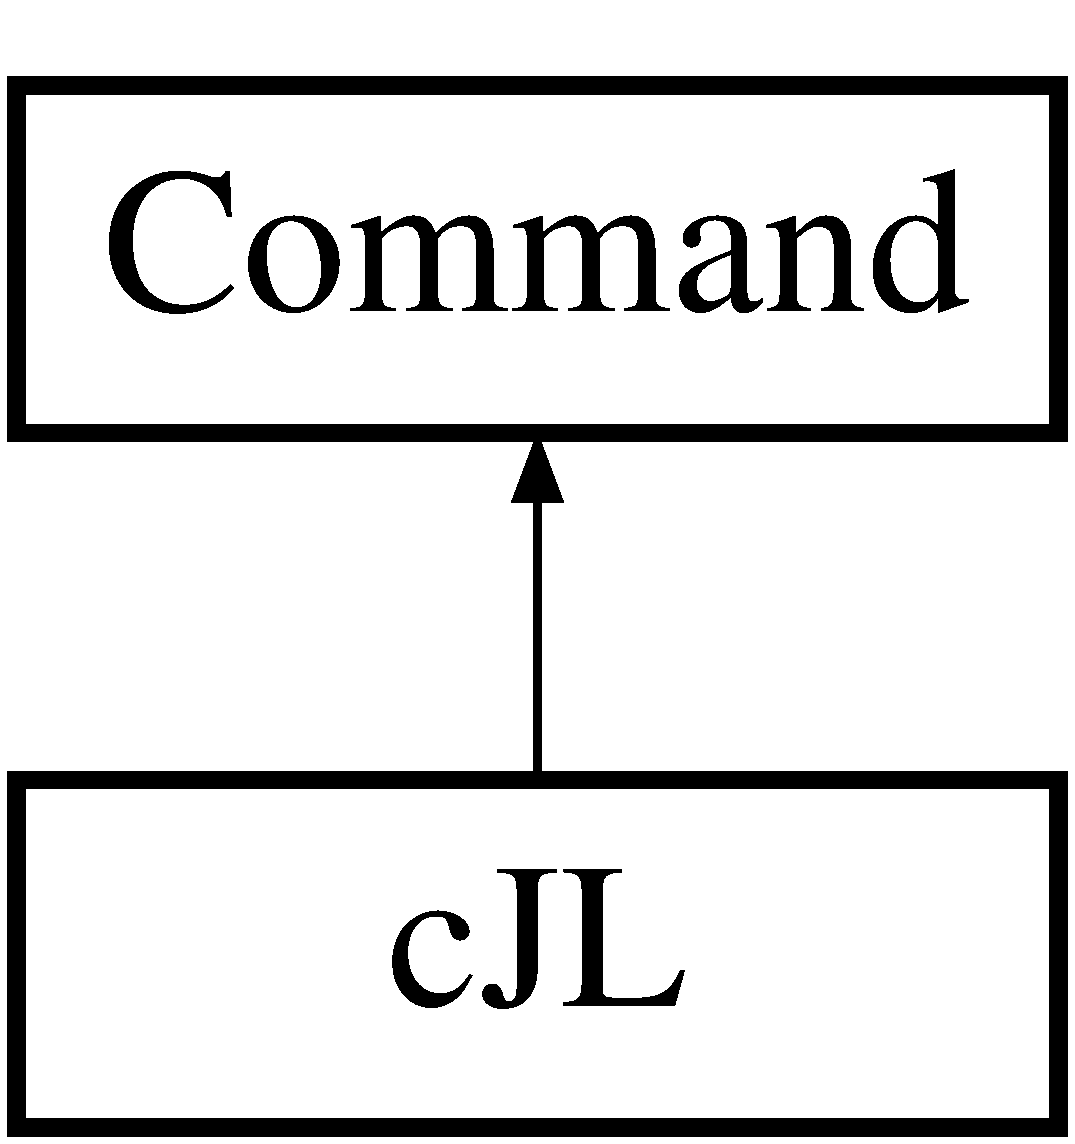
\includegraphics[height=2.000000cm]{classc_j_l}
\end{center}
\end{figure}
\subsection*{Открытые члены}
\begin{DoxyCompactItemize}
\item 
int \hyperlink{classc_j_l_a55b58d0fbac469b387a2e6a4a31902bf}{operator()} (\hyperlink{class_computer}{Computer} $\ast$C\+O\+MP)
\begin{DoxyCompactList}\small\item\em c\+J\+L\+::operator () -\/ Переход если меньше \end{DoxyCompactList}\end{DoxyCompactItemize}
\subsection*{Дополнительные унаследованные члены}


\subsection{Подробное описание}
переход, если меньше 

\subsection{Методы}
\hypertarget{classc_j_l_a55b58d0fbac469b387a2e6a4a31902bf}{}\label{classc_j_l_a55b58d0fbac469b387a2e6a4a31902bf} 
\index{c\+JL@{c\+JL}!operator()@{operator()}}
\index{operator()@{operator()}!c\+JL@{c\+JL}}
\subsubsection{\texorpdfstring{operator()()}{operator()()}}
{\footnotesize\ttfamily int c\+J\+L\+::operator() (\begin{DoxyParamCaption}\item[{\hyperlink{class_computer}{Computer} $\ast$}]{C\+O\+MP }\end{DoxyParamCaption})\hspace{0.3cm}{\ttfamily [virtual]}}



c\+J\+L\+::operator () -\/ Переход если меньше 


\begin{DoxyParams}{Аргументы}
{\em C\+O\+MP} & -\/ указатель на объект компьютер \\
\hline
\end{DoxyParams}
\begin{DoxyReturn}{Возвращает}
1
\end{DoxyReturn}
Если по результатам сравнения Icmp или Rcmp сумматор был меньше адресного регистра, изменяет значение указателя на инструкцию по абсолютному значению адреса ОЗУ, либо отступа от текущего значения. 

Замещает \hyperlink{class_command_a79939b66f3de892e91d7710844294716}{Command}.


\begin{DoxyCode}
390 \{
391     \textcolor{keywordflow}{if}(COMP->\hyperlink{class_computer_aada011a29d87bb979835371a5f09805e}{PSW}.\hyperlink{struct_computer_1_1bits_a74cfe87f17ba348db37c74bbd5e56828}{SF} != 0) \textcolor{keywordflow}{return} 1;
392     \textcolor{keywordflow}{if}(COMP->\hyperlink{class_computer_a8423168f7cc356b4dd36977603798caf}{CMD}.\hyperlink{struct_computer_1_1command_a3e0d1e527de9f60594023a362b08a7de}{B} == 0) \textcolor{comment}{//Абсолютная адресация}
393         COMP->\hyperlink{class_computer_aada011a29d87bb979835371a5f09805e}{PSW}.\hyperlink{struct_computer_1_1bits_a7781883b446209714ad687e2a4f77526}{IP} = COMP->\hyperlink{class_computer_a8423168f7cc356b4dd36977603798caf}{CMD}.\hyperlink{struct_computer_1_1command_a0e07591012953413797506f7bc3cb1a7}{Addr};
394     \textcolor{keywordflow}{else} \textcolor{comment}{//Относит адресация}
395         COMP->\hyperlink{class_computer_aada011a29d87bb979835371a5f09805e}{PSW}.\hyperlink{struct_computer_1_1bits_a7781883b446209714ad687e2a4f77526}{IP} += COMP->\hyperlink{class_computer_a8423168f7cc356b4dd36977603798caf}{CMD}.\hyperlink{struct_computer_1_1command_a0e07591012953413797506f7bc3cb1a7}{Addr};
396 
397     COMP->\hyperlink{class_computer_a10ca6c6b200630119201de16d7368e0f}{debug}(\textcolor{stringliteral}{"Сумматор меньше. Переход по адресу "} + QString::number(COMP->
      \hyperlink{class_computer_aada011a29d87bb979835371a5f09805e}{PSW}.\hyperlink{struct_computer_1_1bits_a7781883b446209714ad687e2a4f77526}{IP}));
398     \textcolor{keywordflow}{return} 1;
399 \}
\end{DoxyCode}


Объявления и описания членов классов находятся в файлах\+:\begin{DoxyCompactItemize}
\item 
C\+:/\+Users/sstarkov/\+Documents/kr\+\_\+\+Interpreter\+V\+M/sources/command.\+h\item 
C\+:/\+Users/sstarkov/\+Documents/kr\+\_\+\+Interpreter\+V\+M/sources/command.\+cpp\end{DoxyCompactItemize}

\hypertarget{classc_jmp}{}\section{Класс c\+Jmp}
\label{classc_jmp}\index{c\+Jmp@{c\+Jmp}}


Безусловный переход  




{\ttfamily \#include $<$command.\+h$>$}

Граф наследования\+:c\+Jmp\+:\begin{figure}[H]
\begin{center}
\leavevmode
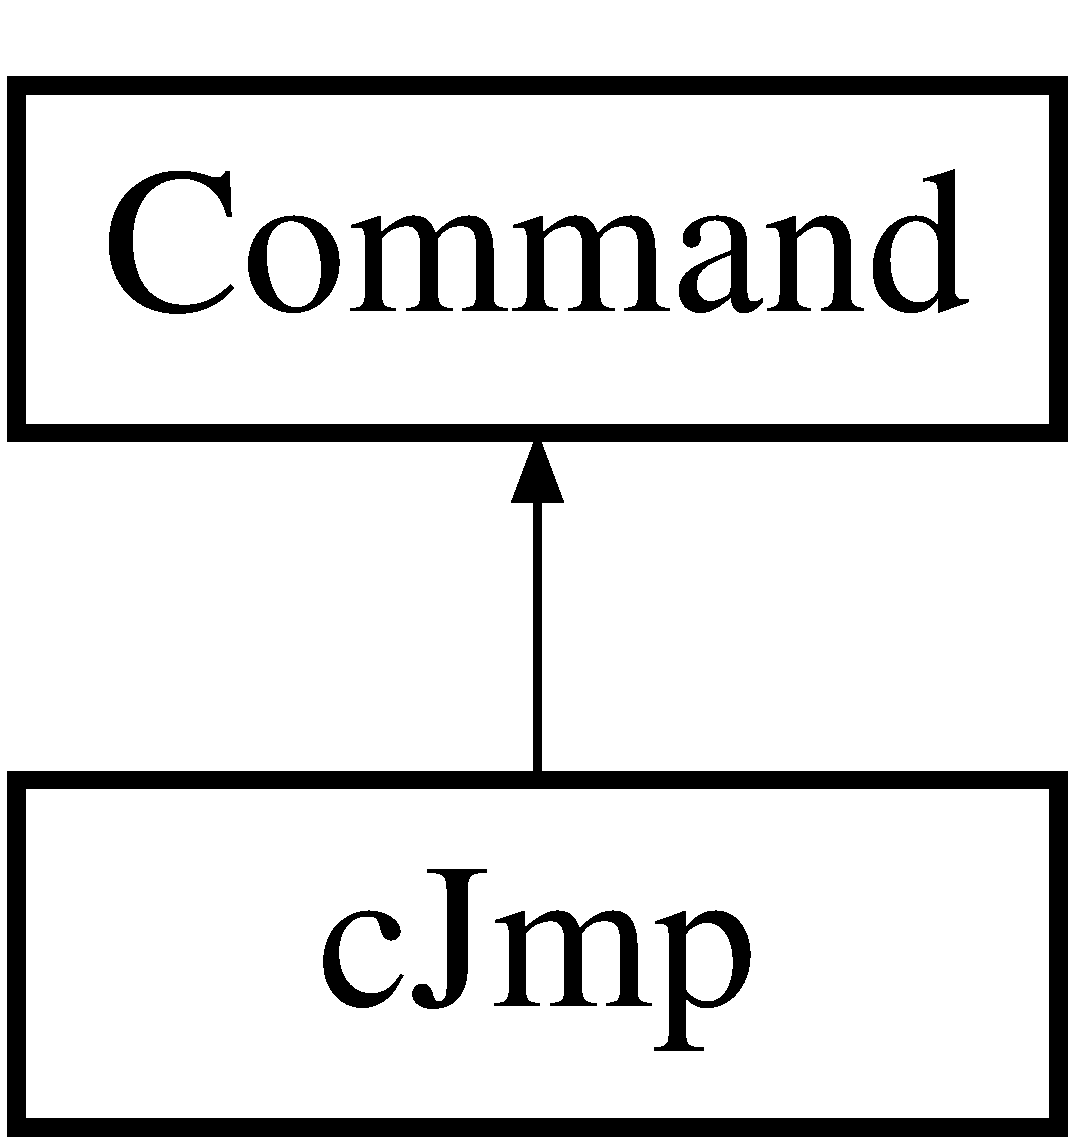
\includegraphics[height=2.000000cm]{classc_jmp}
\end{center}
\end{figure}
\subsection*{Открытые члены}
\begin{DoxyCompactItemize}
\item 
int \hyperlink{classc_jmp_a0da6eb0f611e4793f72cf50a0d788689}{operator()} (\hyperlink{class_computer}{Computer} $\ast$C\+O\+MP)
\begin{DoxyCompactList}\small\item\em c\+Jmp\+::operator () -\/ Безусловный переход \end{DoxyCompactList}\end{DoxyCompactItemize}
\subsection*{Дополнительные унаследованные члены}


\subsection{Подробное описание}
Безусловный переход 

\subsection{Методы}
\hypertarget{classc_jmp_a0da6eb0f611e4793f72cf50a0d788689}{}\label{classc_jmp_a0da6eb0f611e4793f72cf50a0d788689} 
\index{c\+Jmp@{c\+Jmp}!operator()@{operator()}}
\index{operator()@{operator()}!c\+Jmp@{c\+Jmp}}
\subsubsection{\texorpdfstring{operator()()}{operator()()}}
{\footnotesize\ttfamily int c\+Jmp\+::operator() (\begin{DoxyParamCaption}\item[{\hyperlink{class_computer}{Computer} $\ast$}]{C\+O\+MP }\end{DoxyParamCaption})\hspace{0.3cm}{\ttfamily [virtual]}}



c\+Jmp\+::operator () -\/ Безусловный переход 


\begin{DoxyParams}{Аргументы}
{\em C\+O\+MP} & -\/ указатель на объект компьютер \\
\hline
\end{DoxyParams}
\begin{DoxyReturn}{Возвращает}
1
\end{DoxyReturn}
Изменяет значение указателя на инструкцию по абсолютному значению адреса ОЗУ, либо отступа от текущего значения. 

Замещает \hyperlink{class_command_a79939b66f3de892e91d7710844294716}{Command}.


\begin{DoxyCode}
331 \{
332     \textcolor{keywordflow}{if}(COMP->\hyperlink{class_computer_a8423168f7cc356b4dd36977603798caf}{CMD}.\hyperlink{struct_computer_1_1command_a3e0d1e527de9f60594023a362b08a7de}{B} == 0) \textcolor{comment}{//Абсолютная адресация}
333         COMP->\hyperlink{class_computer_aada011a29d87bb979835371a5f09805e}{PSW}.\hyperlink{struct_computer_1_1bits_a7781883b446209714ad687e2a4f77526}{IP} = COMP->\hyperlink{class_computer_a8423168f7cc356b4dd36977603798caf}{CMD}.\hyperlink{struct_computer_1_1command_a0e07591012953413797506f7bc3cb1a7}{Addr};
334     \textcolor{keywordflow}{else} \textcolor{comment}{//Относит адресация}
335         COMP->\hyperlink{class_computer_aada011a29d87bb979835371a5f09805e}{PSW}.\hyperlink{struct_computer_1_1bits_a7781883b446209714ad687e2a4f77526}{IP} += COMP->\hyperlink{class_computer_a8423168f7cc356b4dd36977603798caf}{CMD}.\hyperlink{struct_computer_1_1command_a0e07591012953413797506f7bc3cb1a7}{Addr};
336 
337     COMP->\hyperlink{class_computer_a10ca6c6b200630119201de16d7368e0f}{debug}(\textcolor{stringliteral}{"Безусловный переход по адресу "} + QString::number(COMP->
      \hyperlink{class_computer_aada011a29d87bb979835371a5f09805e}{PSW}.\hyperlink{struct_computer_1_1bits_a7781883b446209714ad687e2a4f77526}{IP}));
338     \textcolor{keywordflow}{return} 1;
339 \}
\end{DoxyCode}


Объявления и описания членов классов находятся в файлах\+:\begin{DoxyCompactItemize}
\item 
C\+:/\+Users/sstarkov/\+Documents/kr\+\_\+\+Interpreter\+V\+M/sources/command.\+h\item 
C\+:/\+Users/sstarkov/\+Documents/kr\+\_\+\+Interpreter\+V\+M/sources/command.\+cpp\end{DoxyCompactItemize}

\hypertarget{classc_j_z}{}\section{Класс c\+JZ}
\label{classc_j_z}\index{c\+JZ@{c\+JZ}}


переход, если ноль (равны)  




{\ttfamily \#include $<$command.\+h$>$}

Граф наследования\+:c\+JZ\+:\begin{figure}[H]
\begin{center}
\leavevmode
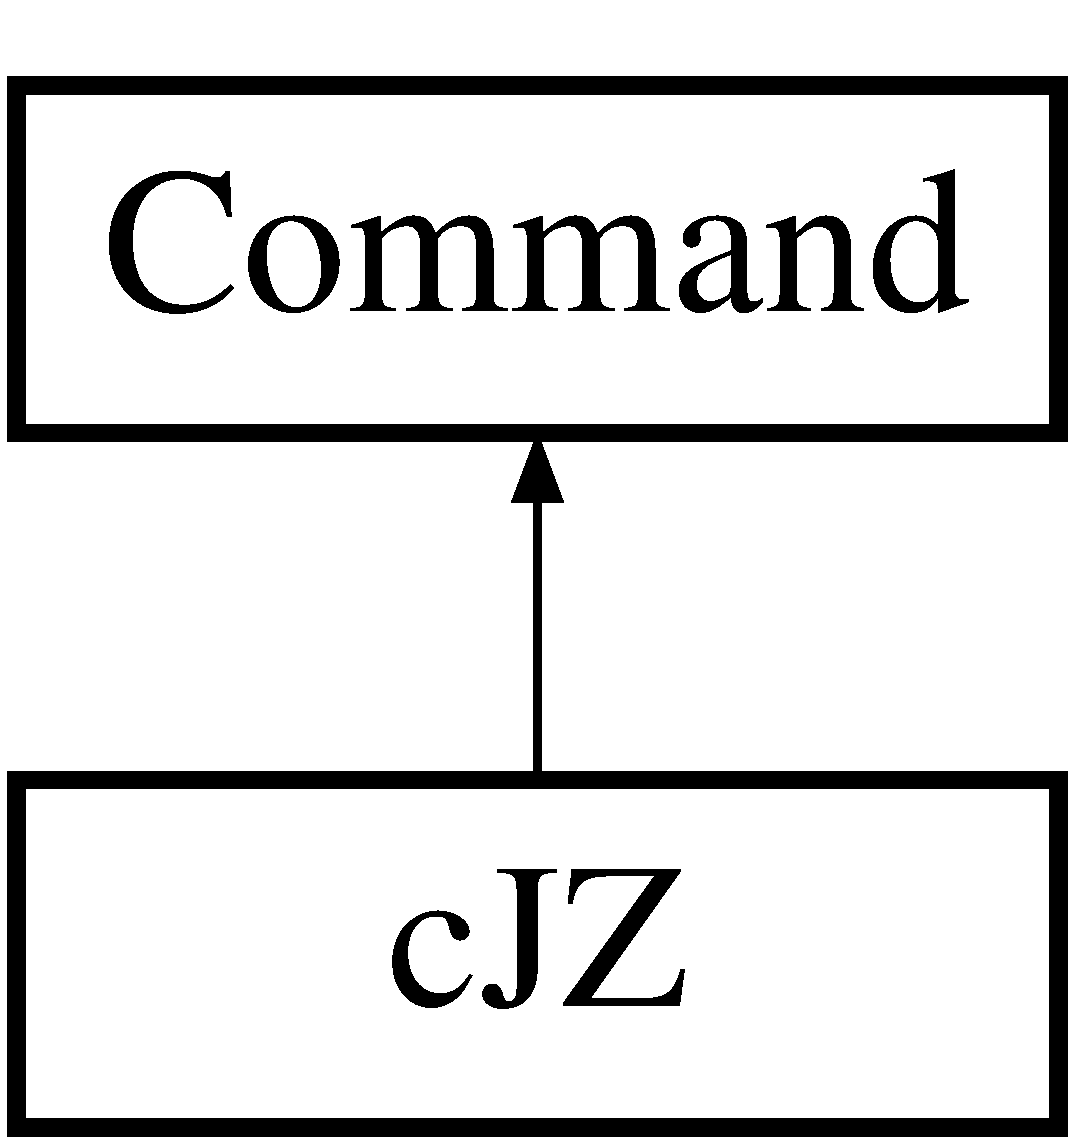
\includegraphics[height=2.000000cm]{classc_j_z}
\end{center}
\end{figure}
\subsection*{Открытые члены}
\begin{DoxyCompactItemize}
\item 
int \hyperlink{classc_j_z_a0887b556d4e1f573e21b2b26588c75e8}{operator()} (\hyperlink{class_computer}{Computer} $\ast$C\+O\+MP)
\begin{DoxyCompactList}\small\item\em c\+J\+Z\+::operator () -\/ Переход если равно \end{DoxyCompactList}\end{DoxyCompactItemize}
\subsection*{Дополнительные унаследованные члены}


\subsection{Подробное описание}
переход, если ноль (равны) 

\subsection{Методы}
\hypertarget{classc_j_z_a0887b556d4e1f573e21b2b26588c75e8}{}\label{classc_j_z_a0887b556d4e1f573e21b2b26588c75e8} 
\index{c\+JZ@{c\+JZ}!operator()@{operator()}}
\index{operator()@{operator()}!c\+JZ@{c\+JZ}}
\subsubsection{\texorpdfstring{operator()()}{operator()()}}
{\footnotesize\ttfamily int c\+J\+Z\+::operator() (\begin{DoxyParamCaption}\item[{\hyperlink{class_computer}{Computer} $\ast$}]{C\+O\+MP }\end{DoxyParamCaption})\hspace{0.3cm}{\ttfamily [virtual]}}



c\+J\+Z\+::operator () -\/ Переход если равно 


\begin{DoxyParams}{Аргументы}
{\em C\+O\+MP} & -\/ указатель на объект компьютер \\
\hline
\end{DoxyParams}
\begin{DoxyReturn}{Возвращает}
1
\end{DoxyReturn}
Если по результатам сравнения Icmp или Rcmp операнды были равны, изменяет значение указателя на инструкцию по абсолютному значению адреса ОЗУ, либо отступа от текущего значения. 

Замещает \hyperlink{class_command_a79939b66f3de892e91d7710844294716}{Command}.


\begin{DoxyCode}
350 \{
351     \textcolor{keywordflow}{if}(COMP->\hyperlink{class_computer_aada011a29d87bb979835371a5f09805e}{PSW}.\hyperlink{struct_computer_1_1bits_a5307edeadd212f1fc19e9f6f5346df39}{ZF} != 1) \textcolor{keywordflow}{return} 1;
352     \textcolor{keywordflow}{if}(COMP->\hyperlink{class_computer_a8423168f7cc356b4dd36977603798caf}{CMD}.\hyperlink{struct_computer_1_1command_a3e0d1e527de9f60594023a362b08a7de}{B} == 0) \textcolor{comment}{//Абсолютная адресация}
353         COMP->\hyperlink{class_computer_aada011a29d87bb979835371a5f09805e}{PSW}.\hyperlink{struct_computer_1_1bits_a7781883b446209714ad687e2a4f77526}{IP} = COMP->\hyperlink{class_computer_a8423168f7cc356b4dd36977603798caf}{CMD}.\hyperlink{struct_computer_1_1command_a0e07591012953413797506f7bc3cb1a7}{Addr};
354     \textcolor{keywordflow}{else} \textcolor{comment}{//Относит адресация}
355         COMP->\hyperlink{class_computer_aada011a29d87bb979835371a5f09805e}{PSW}.\hyperlink{struct_computer_1_1bits_a7781883b446209714ad687e2a4f77526}{IP} += COMP->\hyperlink{class_computer_a8423168f7cc356b4dd36977603798caf}{CMD}.\hyperlink{struct_computer_1_1command_a0e07591012953413797506f7bc3cb1a7}{Addr};
356 
357     COMP->\hyperlink{class_computer_a10ca6c6b200630119201de16d7368e0f}{debug}(\textcolor{stringliteral}{"Операнды равны. Переход по адресу "} + QString::number(COMP->
      \hyperlink{class_computer_aada011a29d87bb979835371a5f09805e}{PSW}.\hyperlink{struct_computer_1_1bits_a7781883b446209714ad687e2a4f77526}{IP}));
358     \textcolor{keywordflow}{return} 1;
359 \}
\end{DoxyCode}


Объявления и описания членов классов находятся в файлах\+:\begin{DoxyCompactItemize}
\item 
C\+:/\+Users/sstarkov/\+Documents/kr\+\_\+\+Interpreter\+V\+M/sources/command.\+h\item 
C\+:/\+Users/sstarkov/\+Documents/kr\+\_\+\+Interpreter\+V\+M/sources/command.\+cpp\end{DoxyCompactItemize}

\hypertarget{classc_load}{}\section{Класс c\+Load}
\label{classc_load}\index{c\+Load@{c\+Load}}


Загрузка сумматора  




{\ttfamily \#include $<$command.\+h$>$}

Граф наследования\+:c\+Load\+:\begin{figure}[H]
\begin{center}
\leavevmode
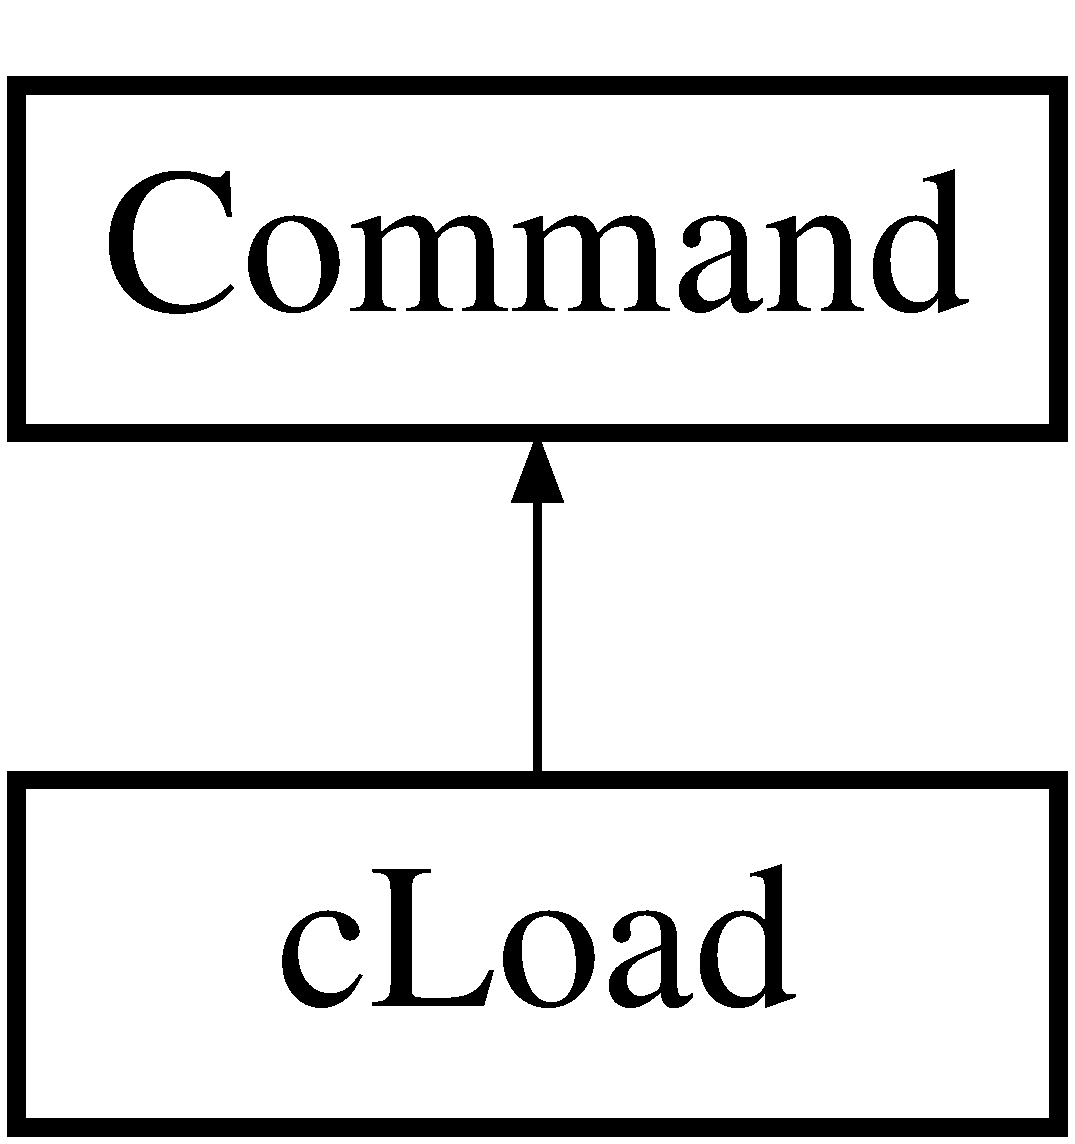
\includegraphics[height=2.000000cm]{classc_load}
\end{center}
\end{figure}
\subsection*{Открытые члены}
\begin{DoxyCompactItemize}
\item 
int \hyperlink{classc_load_a5da79e1b1235b32d87e7f3bd8d1bc00b}{operator()} (\hyperlink{class_computer}{Computer} $\ast$C\+O\+MP)
\begin{DoxyCompactList}\small\item\em c\+Load\+::operator () -\/ Загрузка сумматора \end{DoxyCompactList}\end{DoxyCompactItemize}
\subsection*{Дополнительные унаследованные члены}


\subsection{Подробное описание}
Загрузка сумматора 

\subsection{Методы}
\hypertarget{classc_load_a5da79e1b1235b32d87e7f3bd8d1bc00b}{}\label{classc_load_a5da79e1b1235b32d87e7f3bd8d1bc00b} 
\index{c\+Load@{c\+Load}!operator()@{operator()}}
\index{operator()@{operator()}!c\+Load@{c\+Load}}
\subsubsection{\texorpdfstring{operator()()}{operator()()}}
{\footnotesize\ttfamily int c\+Load\+::operator() (\begin{DoxyParamCaption}\item[{\hyperlink{class_computer}{Computer} $\ast$}]{C\+O\+MP }\end{DoxyParamCaption})\hspace{0.3cm}{\ttfamily [virtual]}}



c\+Load\+::operator () -\/ Загрузка сумматора 


\begin{DoxyParams}{Аргументы}
{\em C\+O\+MP} & -\/ указатель на объект компьютер \\
\hline
\end{DoxyParams}
\begin{DoxyReturn}{Возвращает}
1
\end{DoxyReturn}
Загружает сумматор из ОЗУ. Размер загрузки 4 байта 

Замещает \hyperlink{class_command_a79939b66f3de892e91d7710844294716}{Command}.


\begin{DoxyCode}
217 \{
218     address ptr;
219     \textcolor{keywordflow}{if}(COMP->\hyperlink{class_computer_a8423168f7cc356b4dd36977603798caf}{CMD}.\hyperlink{struct_computer_1_1command_a3e0d1e527de9f60594023a362b08a7de}{B} == 0) \textcolor{comment}{//Абсолютная адресация}
220         ptr =  COMP->\hyperlink{class_computer_a8423168f7cc356b4dd36977603798caf}{CMD}.\hyperlink{struct_computer_1_1command_a0e07591012953413797506f7bc3cb1a7}{Addr};
221     \textcolor{keywordflow}{else} \textcolor{comment}{//Относит адресация}
222         ptr = COMP->\hyperlink{class_computer_a8423168f7cc356b4dd36977603798caf}{CMD}.\hyperlink{struct_computer_1_1command_a0e07591012953413797506f7bc3cb1a7}{Addr} + COMP->\hyperlink{class_computer_a499d0b2c857c2977dd5702906705f79e}{RA};
223 
224     COMP->\hyperlink{class_computer_a10ca6c6b200630119201de16d7368e0f}{debug}(\textcolor{stringliteral}{"Загрузка сумматора из адреса "} + QString::number(ptr));
225 
226     COMP->\hyperlink{class_computer_a874503110664b3cf821118d2ce9c2b96}{RS}.\hyperlink{union_computer_1_1data_a4308eb86abfec2d52028212c599a093b}{b1} = COMP->\hyperlink{class_computer_adcd1bd438b7ad95f043db2acbbd864ae}{MEM}[ptr++];
227     COMP->\hyperlink{class_computer_a874503110664b3cf821118d2ce9c2b96}{RS}.\hyperlink{union_computer_1_1data_a87252409c780b1c387883eb027065709}{b2} = COMP->\hyperlink{class_computer_adcd1bd438b7ad95f043db2acbbd864ae}{MEM}[ptr++];
228     COMP->\hyperlink{class_computer_a874503110664b3cf821118d2ce9c2b96}{RS}.\hyperlink{union_computer_1_1data_af9265f845319a83f5877590e7ab2a497}{b3} = COMP->\hyperlink{class_computer_adcd1bd438b7ad95f043db2acbbd864ae}{MEM}[ptr++];
229     COMP->\hyperlink{class_computer_a874503110664b3cf821118d2ce9c2b96}{RS}.\hyperlink{union_computer_1_1data_aca2c60d7da9da79750a6d3a237dae93c}{b4} = COMP->\hyperlink{class_computer_adcd1bd438b7ad95f043db2acbbd864ae}{MEM}[ptr];
230 
231     \textcolor{keywordflow}{return} 1;
232 \}
\end{DoxyCode}


Объявления и описания членов классов находятся в файлах\+:\begin{DoxyCompactItemize}
\item 
C\+:/\+Users/sstarkov/\+Documents/kr\+\_\+\+Interpreter\+V\+M/sources/command.\+h\item 
C\+:/\+Users/sstarkov/\+Documents/kr\+\_\+\+Interpreter\+V\+M/sources/command.\+cpp\end{DoxyCompactItemize}

\hypertarget{class_command}{}\section{Класс Command}
\label{class_command}\index{Command@{Command}}


Базовый абстрактный класс для паттерна \char`\"{}Комманда\char`\"{}.  




{\ttfamily \#include $<$command.\+h$>$}

Граф наследования\+:Command\+:\begin{figure}[H]
\begin{center}
\leavevmode
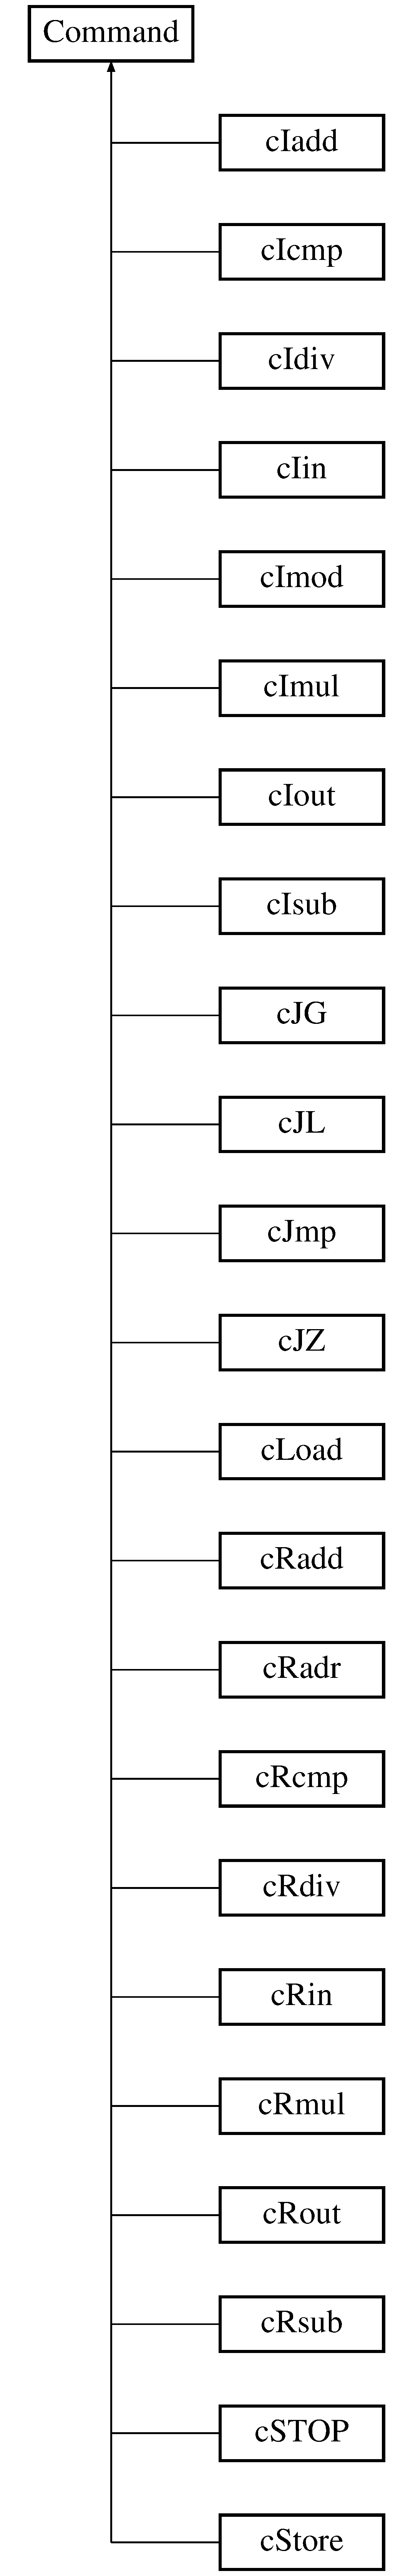
\includegraphics[height=12.000000cm]{class_command}
\end{center}
\end{figure}
\subsection*{Открытые члены}
\begin{DoxyCompactItemize}
\item 
\hypertarget{class_command_a79939b66f3de892e91d7710844294716}{}\label{class_command_a79939b66f3de892e91d7710844294716} 
virtual int \hyperlink{class_command_a79939b66f3de892e91d7710844294716}{operator()} (\hyperlink{class_computer}{Computer} $\ast$)=0
\begin{DoxyCompactList}\small\item\em Перегрузка оператора () \end{DoxyCompactList}\end{DoxyCompactItemize}
\subsection*{Защищенные члены}
\begin{DoxyCompactItemize}
\item 
void \hyperlink{class_command_aac6f368e7c9dbb357b3f00627d5dabfc}{load\+Register} (\hyperlink{class_computer}{Computer} $\ast$C\+O\+MP)
\begin{DoxyCompactList}\small\item\em \hyperlink{class_command_aac6f368e7c9dbb357b3f00627d5dabfc}{Command\+::load\+Register} -\/ загрузка внутреннего регистра \end{DoxyCompactList}\end{DoxyCompactItemize}


\subsection{Подробное описание}
Базовый абстрактный класс для паттерна \char`\"{}Комманда\char`\"{}. 

\subsection{Методы}
\hypertarget{class_command_aac6f368e7c9dbb357b3f00627d5dabfc}{}\label{class_command_aac6f368e7c9dbb357b3f00627d5dabfc} 
\index{Command@{Command}!load\+Register@{load\+Register}}
\index{load\+Register@{load\+Register}!Command@{Command}}
\subsubsection{\texorpdfstring{load\+Register()}{loadRegister()}}
{\footnotesize\ttfamily void Command\+::load\+Register (\begin{DoxyParamCaption}\item[{\hyperlink{class_computer}{Computer} $\ast$}]{C\+O\+MP }\end{DoxyParamCaption})\hspace{0.3cm}{\ttfamily [protected]}}



\hyperlink{class_command_aac6f368e7c9dbb357b3f00627d5dabfc}{Command\+::load\+Register} -\/ загрузка внутреннего регистра 


\begin{DoxyParams}{Аргументы}
{\em C\+O\+MP} & -\/ указатель на объект компьютер\\
\hline
\end{DoxyParams}
Загружает внутренний регистр из адреса по абсолютной или относительной адресации. Функция вызывается только из потомков \hyperlink{class_command}{Command}. 
\begin{DoxyCode}
12 \{
13     \textcolor{keywordtype}{unsigned} \textcolor{keywordtype}{int} ptr;
14     \textcolor{keywordflow}{if}(COMP->\hyperlink{class_computer_a8423168f7cc356b4dd36977603798caf}{CMD}.\hyperlink{struct_computer_1_1command_a3e0d1e527de9f60594023a362b08a7de}{B} == 0) \textcolor{comment}{//Абсолютная адресация}
15         ptr = COMP->\hyperlink{class_computer_a8423168f7cc356b4dd36977603798caf}{CMD}.\hyperlink{struct_computer_1_1command_a0e07591012953413797506f7bc3cb1a7}{Addr};
16     \textcolor{keywordflow}{else} \textcolor{comment}{//Относительная адресация}
17         ptr = COMP->\hyperlink{class_computer_a8423168f7cc356b4dd36977603798caf}{CMD}.\hyperlink{struct_computer_1_1command_a0e07591012953413797506f7bc3cb1a7}{Addr} + COMP->\hyperlink{class_computer_a499d0b2c857c2977dd5702906705f79e}{RA};
18     COMP->\hyperlink{class_computer_a10ca6c6b200630119201de16d7368e0f}{debug}(\textcolor{stringliteral}{"Загрузка регистра из адреса "} + QString::number(ptr));
19 
20     COMP->\hyperlink{class_computer_a0fbf84599b7db9d634a92afed443ee73}{R1}.\hyperlink{union_computer_1_1data_a4308eb86abfec2d52028212c599a093b}{b1} = COMP->\hyperlink{class_computer_adcd1bd438b7ad95f043db2acbbd864ae}{MEM}[ptr++];
21     COMP->\hyperlink{class_computer_a0fbf84599b7db9d634a92afed443ee73}{R1}.\hyperlink{union_computer_1_1data_a87252409c780b1c387883eb027065709}{b2} = COMP->\hyperlink{class_computer_adcd1bd438b7ad95f043db2acbbd864ae}{MEM}[ptr++];
22     COMP->\hyperlink{class_computer_a0fbf84599b7db9d634a92afed443ee73}{R1}.\hyperlink{union_computer_1_1data_af9265f845319a83f5877590e7ab2a497}{b3} = COMP->\hyperlink{class_computer_adcd1bd438b7ad95f043db2acbbd864ae}{MEM}[ptr++];
23     COMP->\hyperlink{class_computer_a0fbf84599b7db9d634a92afed443ee73}{R1}.\hyperlink{union_computer_1_1data_aca2c60d7da9da79750a6d3a237dae93c}{b4} = COMP->\hyperlink{class_computer_adcd1bd438b7ad95f043db2acbbd864ae}{MEM}[ptr++];    
24 \}
\end{DoxyCode}


Объявления и описания членов классов находятся в файлах\+:\begin{DoxyCompactItemize}
\item 
C\+:/\+Users/sstarkov/\+Documents/kr\+\_\+\+Interpreter\+V\+M/sources/command.\+h\item 
C\+:/\+Users/sstarkov/\+Documents/kr\+\_\+\+Interpreter\+V\+M/sources/command.\+cpp\end{DoxyCompactItemize}

\hypertarget{struct_computer_1_1command}{}\section{Структура Computer\+:\+:command}
\label{struct_computer_1_1command}\index{Computer\+::command@{Computer\+::command}}


command struct -\/ структура команды для выполнения. 3 байта.  


\subsection*{Открытые атрибуты}
\begin{DoxyCompactItemize}
\item 
\hypertarget{struct_computer_1_1command_abab9a57c8c7fcd2f70c6a3e082e29032}{}\label{struct_computer_1_1command_abab9a57c8c7fcd2f70c6a3e082e29032} 
\begin{tabbing}
xx\=xx\=xx\=xx\=xx\=xx\=xx\=xx\=xx\=\kill
union \{\\
\>byte \hyperlink{struct_computer_1_1command_afd02c65efae303e5c528aab2eaa17556}{Cmd}\\
\>\>{\em код операции 1 байт в флагом адресации на старшем бите }\\
\hypertarget{union_computer_1_1command_1_1_0D0_ab80c892093be4d5b8271cb0ea2275b90}{}\label{union_computer_1_1command_1_1_0D0_ab80c892093be4d5b8271cb0ea2275b90} 
\>struct \{\\
\>\>bit \hyperlink{struct_computer_1_1command_a2714eda12dcfba46770769c7ed9c7f0a}{OP}:7\\
\>\>\>{\em Код операции }\\
\>\>bit \hyperlink{struct_computer_1_1command_a3e0d1e527de9f60594023a362b08a7de}{B}:1\\
\>\>\>{\em Флаг адресации }\\
\>\} \\
\}; \\

\end{tabbing}\item 
\hypertarget{struct_computer_1_1command_aea8343f26b8cf44fe3f684579bca1a12}{}\label{struct_computer_1_1command_aea8343f26b8cf44fe3f684579bca1a12} 
\begin{tabbing}
xx\=xx\=xx\=xx\=xx\=xx\=xx\=xx\=xx\=\kill
union \{\\
\>address \hyperlink{struct_computer_1_1command_a0e07591012953413797506f7bc3cb1a7}{Addr}\\
\>\>{\em Адрес аргумента }\\
\hypertarget{union_computer_1_1command_1_1_0D2_adb09ec420e7388614fefa31fb49e6320}{}\label{union_computer_1_1command_1_1_0D2_adb09ec420e7388614fefa31fb49e6320} 
\>struct \{\\
\>\>byte \hyperlink{struct_computer_1_1command_a840bf646fc591a80cd94f253bb8cae02}{H\_Addr}\\
\>\>\>{\em Старший байт }\\
\>\>byte \hyperlink{struct_computer_1_1command_afe8e3496cc61746a889f53f91ed66d45}{L\_Addr}\\
\>\>\>{\em Младший байт }\\
\>\} \\
\}; \\

\end{tabbing}\end{DoxyCompactItemize}


\subsection{Подробное описание}
command struct -\/ структура команды для выполнения. 3 байта. 

Структура команды процессора. 3 байта. 

Объявления и описания членов структуры находятся в файле\+:\begin{DoxyCompactItemize}
\item 
C\+:/\+Users/sstarkov/\+Documents/kr\+\_\+\+Interpreter\+V\+M/sources/computer.\+h\end{DoxyCompactItemize}

\hypertarget{class_computer}{}\section{Класс Computer}
\label{class_computer}\index{Computer@{Computer}}


Класс \hyperlink{class_computer}{Computer} реализует архитектуру компьютера  




{\ttfamily \#include $<$computer.\+h$>$}

\subsection*{Классы}
\begin{DoxyCompactItemize}
\item 
struct \hyperlink{struct_computer_1_1bits}{bits}
\begin{DoxyCompactList}\small\item\em P\+SW (Cостояние процессора) \end{DoxyCompactList}\item 
struct \hyperlink{struct_computer_1_1command}{command}
\begin{DoxyCompactList}\small\item\em command struct -\/ структура команды для выполнения. 3 байта. \end{DoxyCompactList}\item 
union \hyperlink{union_computer_1_1data}{data}
\begin{DoxyCompactList}\small\item\em data union -\/ структура данных 4 байта \end{DoxyCompactList}\end{DoxyCompactItemize}
\subsection*{Открытые члены}
\begin{DoxyCompactItemize}
\item 
\hyperlink{class_computer_ae13c32fa07ad956f0c229608dab5e332}{Computer} (Q\+String P\+A\+TH, \hyperlink{classinterpreter}{interpreter} $\ast$I\+N\+T\+ER)
\begin{DoxyCompactList}\small\item\em \hyperlink{class_computer_ae13c32fa07ad956f0c229608dab5e332}{Computer\+::\+Computer} -\/ конструктор \end{DoxyCompactList}\item 
int \hyperlink{class_computer_a4303af6a549fc8f792de0d2d18a9e05f}{execute} ()
\begin{DoxyCompactList}\small\item\em Запуск выполнения программы \end{DoxyCompactList}\end{DoxyCompactItemize}
\subsection*{Закрытые члены}
\begin{DoxyCompactItemize}
\item 
void \hyperlink{class_computer_aa57b0ed2f3a9b168c2924174ec524bd4}{interrupt} (int interrupt\+Code)
\begin{DoxyCompactList}\small\item\em Обработчик прерываний \end{DoxyCompactList}\item 
void \hyperlink{class_computer_a10ca6c6b200630119201de16d7368e0f}{debug} (Q\+String)
\begin{DoxyCompactList}\small\item\em Передача сообщения для последующего вывода в лог \end{DoxyCompactList}\item 
void \hyperlink{class_computer_aeab90cbacbef385685717c249a07929d}{reset} ()
\begin{DoxyCompactList}\small\item\em сброс регистров \end{DoxyCompactList}\item 
bool \hyperlink{class_computer_adeb4bbeee2b9c13616dc8c4ef52cbe60}{load} ()
\begin{DoxyCompactList}\small\item\em Загрузка программы \end{DoxyCompactList}\item 
int \hyperlink{class_computer_af337e329e3bc6d80bbd7070e25ce5731}{run} ()
\begin{DoxyCompactList}\small\item\em Основной цикл процессора \end{DoxyCompactList}\item 
void \hyperlink{class_computer_aae4a76a8a03a6c9fb1c12968d629be3e}{flagI} ()
\begin{DoxyCompactList}\small\item\em Установка флагов для целого числа \end{DoxyCompactList}\item 
void \hyperlink{class_computer_aae860bb217270ec88e8ebf6fe2c2adc9}{flagR} ()
\begin{DoxyCompactList}\small\item\em Установка флагов для вещественного числа \end{DoxyCompactList}\end{DoxyCompactItemize}
\subsection*{Закрытые данные}
\begin{DoxyCompactItemize}
\item 
\hyperlink{classinterpreter}{interpreter} $\ast$ \hyperlink{class_computer_aa58d6e565412d6705657c0418b1e59fe}{Interpreter}
\begin{DoxyCompactList}\small\item\em Interpreter -\/ Указатель на родителя \end{DoxyCompactList}\item 
\hypertarget{class_computer_a05fb0474bddcf52789780fd6457cefac}{}\label{class_computer_a05fb0474bddcf52789780fd6457cefac} 
Q\+String \hyperlink{class_computer_a05fb0474bddcf52789780fd6457cefac}{program\+Path}
\begin{DoxyCompactList}\small\item\em program\+Path -\/ Путь до файла с программой, которую нужно выполнить \end{DoxyCompactList}\item 
\hypertarget{class_computer_a8423168f7cc356b4dd36977603798caf}{}\label{class_computer_a8423168f7cc356b4dd36977603798caf} 
struct \hyperlink{struct_computer_1_1command}{Computer\+::command} \hyperlink{class_computer_a8423168f7cc356b4dd36977603798caf}{C\+MD}
\begin{DoxyCompactList}\small\item\em Объект структуры команды \end{DoxyCompactList}\item 
\hypertarget{class_computer_adb154047da2156e4419af3b3a4a766b7}{}\label{class_computer_adb154047da2156e4419af3b3a4a766b7} 
union \hyperlink{union_computer_1_1data}{Computer\+::data} \hyperlink{class_computer_adb154047da2156e4419af3b3a4a766b7}{D\+A\+TA}
\begin{DoxyCompactList}\small\item\em Объект структуры данных \end{DoxyCompactList}\item 
\hypertarget{class_computer_aada011a29d87bb979835371a5f09805e}{}\label{class_computer_aada011a29d87bb979835371a5f09805e} 
struct \hyperlink{struct_computer_1_1bits}{Computer\+::bits} \hyperlink{class_computer_aada011a29d87bb979835371a5f09805e}{P\+SW}
\begin{DoxyCompactList}\small\item\em Объект структуры состояния процессора \end{DoxyCompactList}\item 
\hypertarget{class_computer_a297a9b79381a9f2005c574f09ea73d70}{}\label{class_computer_a297a9b79381a9f2005c574f09ea73d70} 
\hyperlink{class_command}{Command} $\ast$ \hyperlink{class_computer_a297a9b79381a9f2005c574f09ea73d70}{p\+C\+MD} \mbox{[}128\mbox{]} = \{nullptr\}
\begin{DoxyCompactList}\small\item\em набор команд процессора, инициализируется в конструкторе \end{DoxyCompactList}\item 
\hypertarget{class_computer_a874503110664b3cf821118d2ce9c2b96}{}\label{class_computer_a874503110664b3cf821118d2ce9c2b96} 
\hyperlink{union_computer_1_1data}{data} \hyperlink{class_computer_a874503110664b3cf821118d2ce9c2b96}{RS}
\begin{DoxyCompactList}\small\item\em Сумматор 4 байта \end{DoxyCompactList}\item 
\hypertarget{class_computer_a499d0b2c857c2977dd5702906705f79e}{}\label{class_computer_a499d0b2c857c2977dd5702906705f79e} 
address \hyperlink{class_computer_a499d0b2c857c2977dd5702906705f79e}{RA}
\begin{DoxyCompactList}\small\item\em Адресный регистр 2 байта \end{DoxyCompactList}\item 
\hypertarget{class_computer_a0fbf84599b7db9d634a92afed443ee73}{}\label{class_computer_a0fbf84599b7db9d634a92afed443ee73} 
\hyperlink{union_computer_1_1data}{data} \hyperlink{class_computer_a0fbf84599b7db9d634a92afed443ee73}{R1}
\begin{DoxyCompactList}\small\item\em Внутренний регистр \end{DoxyCompactList}\item 
byte $\ast$ \hyperlink{class_computer_adcd1bd438b7ad95f043db2acbbd864ae}{M\+EM} = new byte\mbox{[}0xffff\mbox{]}
\begin{DoxyCompactList}\small\item\em M\+EM -\/ Оперативная память \end{DoxyCompactList}\end{DoxyCompactItemize}
\subsection*{Друзья}
\begin{DoxyCompactItemize}
\item 
\hypertarget{class_computer_a62a7fc89f0ee4604e3ccab9b6b6a343f}{}\label{class_computer_a62a7fc89f0ee4604e3ccab9b6b6a343f} 
class {\bfseries Command}
\item 
\hypertarget{class_computer_af5200c1b25e6d6c70149aeb43469862d}{}\label{class_computer_af5200c1b25e6d6c70149aeb43469862d} 
class {\bfseries c\+Iadd}
\item 
\hypertarget{class_computer_a34690541a879c55084846d0cc959f663}{}\label{class_computer_a34690541a879c55084846d0cc959f663} 
class {\bfseries c\+Radd}
\item 
\hypertarget{class_computer_acb4f2916d54a02a5aa6916c3dde9b9ad}{}\label{class_computer_acb4f2916d54a02a5aa6916c3dde9b9ad} 
class {\bfseries c\+Isub}
\item 
\hypertarget{class_computer_a8a74408651dfcb80351e8a528cc7e313}{}\label{class_computer_a8a74408651dfcb80351e8a528cc7e313} 
class {\bfseries c\+Rsub}
\item 
\hypertarget{class_computer_a403b0571c72075bde36e9a03510eff49}{}\label{class_computer_a403b0571c72075bde36e9a03510eff49} 
class {\bfseries c\+Imul}
\item 
\hypertarget{class_computer_a92e22a42f3315bfac267253edcd011e6}{}\label{class_computer_a92e22a42f3315bfac267253edcd011e6} 
class {\bfseries c\+Rmul}
\item 
\hypertarget{class_computer_a8eccf947fdd09a055e4f096329babc93}{}\label{class_computer_a8eccf947fdd09a055e4f096329babc93} 
class {\bfseries c\+Idiv}
\item 
\hypertarget{class_computer_a5783b61b2e06d3ae070dec6726528dca}{}\label{class_computer_a5783b61b2e06d3ae070dec6726528dca} 
class {\bfseries c\+Rdiv}
\item 
\hypertarget{class_computer_a58a26d915580e452f8ebf5f5c35ec102}{}\label{class_computer_a58a26d915580e452f8ebf5f5c35ec102} 
class {\bfseries c\+Imod}
\item 
\hypertarget{class_computer_add13bd38b4e1ceb581c8aafdd18d6a38}{}\label{class_computer_add13bd38b4e1ceb581c8aafdd18d6a38} 
class {\bfseries c\+Radr}
\item 
\hypertarget{class_computer_a06f50956cd4489638e7658659729566b}{}\label{class_computer_a06f50956cd4489638e7658659729566b} 
class {\bfseries c\+Load}
\item 
\hypertarget{class_computer_ae67eb3dc4175713f1a79f74bd1d03eed}{}\label{class_computer_ae67eb3dc4175713f1a79f74bd1d03eed} 
class {\bfseries c\+Store}
\item 
\hypertarget{class_computer_accaf41340be465f8a862e40429ba9cfb}{}\label{class_computer_accaf41340be465f8a862e40429ba9cfb} 
class {\bfseries c\+Jmp}
\item 
\hypertarget{class_computer_af7af8f966cd39d199ce18113ecdd2ecb}{}\label{class_computer_af7af8f966cd39d199ce18113ecdd2ecb} 
class {\bfseries c\+Icmp}
\item 
\hypertarget{class_computer_a7c711c41af5fcddc63bc8e8c41f620f4}{}\label{class_computer_a7c711c41af5fcddc63bc8e8c41f620f4} 
class {\bfseries c\+Rcmp}
\item 
\hypertarget{class_computer_a784d5ff4da579d46119d42608ee66334}{}\label{class_computer_a784d5ff4da579d46119d42608ee66334} 
class {\bfseries c\+JZ}
\item 
\hypertarget{class_computer_a3adfd5a9699d8611e902f47cbdfc34d1}{}\label{class_computer_a3adfd5a9699d8611e902f47cbdfc34d1} 
class {\bfseries c\+JG}
\item 
\hypertarget{class_computer_a69be74228435ed08e42c04d34abd383a}{}\label{class_computer_a69be74228435ed08e42c04d34abd383a} 
class {\bfseries c\+JL}
\item 
\hypertarget{class_computer_a0b86d0871da7c7632d6c45491faae5ab}{}\label{class_computer_a0b86d0871da7c7632d6c45491faae5ab} 
class {\bfseries c\+Iin}
\item 
\hypertarget{class_computer_a02eb85182aba14840a06c5d5f9c4a4e4}{}\label{class_computer_a02eb85182aba14840a06c5d5f9c4a4e4} 
class {\bfseries c\+Iout}
\item 
\hypertarget{class_computer_a047a81456a9fc5a1160d96ac296fd762}{}\label{class_computer_a047a81456a9fc5a1160d96ac296fd762} 
class {\bfseries c\+Rin}
\item 
\hypertarget{class_computer_ad68469c232d5ffab3e425a9f058b9168}{}\label{class_computer_ad68469c232d5ffab3e425a9f058b9168} 
class {\bfseries c\+Rout}
\end{DoxyCompactItemize}


\subsection{Подробное описание}
Класс \hyperlink{class_computer}{Computer} реализует архитектуру компьютера 

Содержит в себе реализацию регистров, памяти, и т.\+д. 

\subsection{Конструктор(ы)}
\hypertarget{class_computer_ae13c32fa07ad956f0c229608dab5e332}{}\label{class_computer_ae13c32fa07ad956f0c229608dab5e332} 
\index{Computer@{Computer}!Computer@{Computer}}
\index{Computer@{Computer}!Computer@{Computer}}
\subsubsection{\texorpdfstring{Computer()}{Computer()}}
{\footnotesize\ttfamily Computer\+::\+Computer (\begin{DoxyParamCaption}\item[{Q\+String}]{P\+A\+TH,  }\item[{\hyperlink{classinterpreter}{interpreter} $\ast$}]{I\+N\+T\+ER }\end{DoxyParamCaption})}



\hyperlink{class_computer_ae13c32fa07ad956f0c229608dab5e332}{Computer\+::\+Computer} -\/ конструктор 


\begin{DoxyParams}{Аргументы}
{\em P\+A\+TH} & -\/ путь до файла программы \\
\hline
{\em I\+N\+T\+ER} & -\/ указатель на объект родитель\\
\hline
\end{DoxyParams}
Инициализирует массив команд процессора, и переменные. 
\begin{DoxyCode}
13 \{
14     \hyperlink{class_computer_a05fb0474bddcf52789780fd6457cefac}{programPath} = PATH;     \textcolor{comment}{//Путь до программы}
15     \hyperlink{class_computer_aa58d6e565412d6705657c0418b1e59fe}{Interpreter} = INTER;    \textcolor{comment}{//Указатель на родителя}
16 
17     \hyperlink{class_computer_a297a9b79381a9f2005c574f09ea73d70}{pCMD}[STOP]  =   \textcolor{keyword}{new} \hyperlink{classc_s_t_o_p}{cSTOP}();    \textcolor{comment}{//Остановка}
18 
19     \textcolor{comment}{//Целая арифметика}
20     \hyperlink{class_computer_a297a9b79381a9f2005c574f09ea73d70}{pCMD}[Iadd]  =   \textcolor{keyword}{new} \hyperlink{classc_iadd}{cIadd}();    \textcolor{comment}{//Целочисленное сложение}
21     \hyperlink{class_computer_a297a9b79381a9f2005c574f09ea73d70}{pCMD}[Isub]  =   \textcolor{keyword}{new} \hyperlink{classc_isub}{cIsub}();    \textcolor{comment}{//Целочисленное вычитание}
22     \hyperlink{class_computer_a297a9b79381a9f2005c574f09ea73d70}{pCMD}[Imul]  =   \textcolor{keyword}{new} \hyperlink{classc_imul}{cImul}();    \textcolor{comment}{//Целочисленное умножение}
23     \hyperlink{class_computer_a297a9b79381a9f2005c574f09ea73d70}{pCMD}[Idiv]  =   \textcolor{keyword}{new} \hyperlink{classc_idiv}{cIdiv}();    \textcolor{comment}{//Целочисленное деление}
24     \hyperlink{class_computer_a297a9b79381a9f2005c574f09ea73d70}{pCMD}[Imod]  =   \textcolor{keyword}{new} \hyperlink{classc_imod}{cImod}();    \textcolor{comment}{//Целочисл. остаток от деления}
25     \hyperlink{class_computer_a297a9b79381a9f2005c574f09ea73d70}{pCMD}[Iin]   =   \textcolor{keyword}{new} \hyperlink{classc_iin}{cIin}();     \textcolor{comment}{//Ввод целого числа}
26     \hyperlink{class_computer_a297a9b79381a9f2005c574f09ea73d70}{pCMD}[Iout]  =   \textcolor{keyword}{new} \hyperlink{classc_iout}{cIout}();    \textcolor{comment}{//Вывод целого числа}
27 
28     \textcolor{comment}{//Дробная арифметика}
29     \hyperlink{class_computer_a297a9b79381a9f2005c574f09ea73d70}{pCMD}[Radd]  =   \textcolor{keyword}{new} \hyperlink{classc_radd}{cRadd}();    \textcolor{comment}{//Вещественное сложение}
30     \hyperlink{class_computer_a297a9b79381a9f2005c574f09ea73d70}{pCMD}[Rsub]  =   \textcolor{keyword}{new} \hyperlink{classc_rsub}{cRsub}();    \textcolor{comment}{//Вещественное вычитание}
31     \hyperlink{class_computer_a297a9b79381a9f2005c574f09ea73d70}{pCMD}[Rmul]  =   \textcolor{keyword}{new} \hyperlink{classc_rmul}{cRmul}();    \textcolor{comment}{//Вещественное умножение}
32     \hyperlink{class_computer_a297a9b79381a9f2005c574f09ea73d70}{pCMD}[Rdiv]  =   \textcolor{keyword}{new} \hyperlink{classc_rdiv}{cRdiv}();    \textcolor{comment}{//Вещественное деление}
33     \hyperlink{class_computer_a297a9b79381a9f2005c574f09ea73d70}{pCMD}[Rin]   =   \textcolor{keyword}{new} \hyperlink{classc_rin}{cRin}();     \textcolor{comment}{//Ввод вещественного числа}
34     \hyperlink{class_computer_a297a9b79381a9f2005c574f09ea73d70}{pCMD}[Rout]  =   \textcolor{keyword}{new} \hyperlink{classc_rout}{cRout}();    \textcolor{comment}{//Вывод вещественного числа}
35 
36     \textcolor{comment}{//Операции с сумматором}
37     \hyperlink{class_computer_a297a9b79381a9f2005c574f09ea73d70}{pCMD}[Load]  =   \textcolor{keyword}{new} \hyperlink{classc_load}{cLoad}();    \textcolor{comment}{//Загрузка сумматора}
38     \hyperlink{class_computer_a297a9b79381a9f2005c574f09ea73d70}{pCMD}[Store] =   \textcolor{keyword}{new} \hyperlink{classc_store}{cStore}();   \textcolor{comment}{//Сохранение сумматора}
39 
40     \hyperlink{class_computer_a297a9b79381a9f2005c574f09ea73d70}{pCMD}[Radr]  =   \textcolor{keyword}{new} \hyperlink{classc_radr}{cRadr}();    \textcolor{comment}{//Загрузка адресного регистра константой}
41 
42     \textcolor{comment}{//прыжки}
43     \hyperlink{class_computer_a297a9b79381a9f2005c574f09ea73d70}{pCMD}[Jmp]   =   \textcolor{keyword}{new} \hyperlink{classc_jmp}{cJmp}();     \textcolor{comment}{//Безусловный переход}
44     \hyperlink{class_computer_a297a9b79381a9f2005c574f09ea73d70}{pCMD}[JZ]    =   \textcolor{keyword}{new} \hyperlink{classc_j_z}{cJZ}();      \textcolor{comment}{// ==}
45     \hyperlink{class_computer_a297a9b79381a9f2005c574f09ea73d70}{pCMD}[JG]    =   \textcolor{keyword}{new} \hyperlink{classc_j_g}{cJG}();      \textcolor{comment}{// >}
46     \hyperlink{class_computer_a297a9b79381a9f2005c574f09ea73d70}{pCMD}[JL]    =   \textcolor{keyword}{new} \hyperlink{classc_j_l}{cJL}();      \textcolor{comment}{// <}
47 
48     \textcolor{comment}{//сравнение cIcmp}
49     \hyperlink{class_computer_a297a9b79381a9f2005c574f09ea73d70}{pCMD}[Icmp]  =   \textcolor{keyword}{new} \hyperlink{classc_icmp}{cIcmp}();    \textcolor{comment}{//Целочисленное сравнение}
50     \hyperlink{class_computer_a297a9b79381a9f2005c574f09ea73d70}{pCMD}[Rcmp]  =   \textcolor{keyword}{new} \hyperlink{classc_rcmp}{cRcmp}();    \textcolor{comment}{//Вещественное сравнение}
51 \}
\end{DoxyCode}


\subsection{Методы}
\hypertarget{class_computer_a10ca6c6b200630119201de16d7368e0f}{}\label{class_computer_a10ca6c6b200630119201de16d7368e0f} 
\index{Computer@{Computer}!debug@{debug}}
\index{debug@{debug}!Computer@{Computer}}
\subsubsection{\texorpdfstring{debug()}{debug()}}
{\footnotesize\ttfamily void Computer\+::debug (\begin{DoxyParamCaption}\item[{Q\+String}]{msg }\end{DoxyParamCaption})\hspace{0.3cm}{\ttfamily [private]}}



Передача сообщения для последующего вывода в лог 

\hyperlink{class_computer_a10ca6c6b200630119201de16d7368e0f}{Computer\+::debug} -\/ Отладочное сообщение


\begin{DoxyParams}{Аргументы}
{\em msg} & -\/ Текст сообщения\\
\hline
\end{DoxyParams}
Отправляет текст отладочного сообщения интерпретатору 
\begin{DoxyCode}
222 \{
223     \hyperlink{class_computer_aa58d6e565412d6705657c0418b1e59fe}{Interpreter}->\hyperlink{classinterpreter_a5153712027e3e4344f72336f8b5cfa6d}{debug}(msg);
224 \}
\end{DoxyCode}
\hypertarget{class_computer_a4303af6a549fc8f792de0d2d18a9e05f}{}\label{class_computer_a4303af6a549fc8f792de0d2d18a9e05f} 
\index{Computer@{Computer}!execute@{execute}}
\index{execute@{execute}!Computer@{Computer}}
\subsubsection{\texorpdfstring{execute()}{execute()}}
{\footnotesize\ttfamily int Computer\+::execute (\begin{DoxyParamCaption}{ }\end{DoxyParamCaption})}



Запуск выполнения программы 

\hyperlink{class_computer_a4303af6a549fc8f792de0d2d18a9e05f}{Computer\+::execute} -\/ алгоритм запуска программы

\begin{DoxyReturn}{Возвращает}
Код завершения выполнения программы
\end{DoxyReturn}
Сбрасывает регистры. Загружает программу в память. Запускает прцессор. 
\begin{DoxyCode}
175 \{
176     this->\hyperlink{class_computer_aeab90cbacbef385685717c249a07929d}{reset}();
177     \textcolor{keywordflow}{if}(!this->\hyperlink{class_computer_adeb4bbeee2b9c13616dc8c4ef52cbe60}{load}())
178     \{
179         \textcolor{keywordflow}{return} 2;
180     \}
181     \textcolor{keywordflow}{return} this->\hyperlink{class_computer_af337e329e3bc6d80bbd7070e25ce5731}{run}();
182 \}
\end{DoxyCode}
\hypertarget{class_computer_aae4a76a8a03a6c9fb1c12968d629be3e}{}\label{class_computer_aae4a76a8a03a6c9fb1c12968d629be3e} 
\index{Computer@{Computer}!flagI@{flagI}}
\index{flagI@{flagI}!Computer@{Computer}}
\subsubsection{\texorpdfstring{flag\+I()}{flagI()}}
{\footnotesize\ttfamily void Computer\+::flagI (\begin{DoxyParamCaption}{ }\end{DoxyParamCaption})\hspace{0.3cm}{\ttfamily [private]}}



Установка флагов для целого числа 

\hyperlink{class_computer_aae4a76a8a03a6c9fb1c12968d629be3e}{Computer\+::flagI} -\/ Установка флага для целых чисел

Устанавливает флаги для целочисленного сумматора 
\begin{DoxyCode}
146 \{
147     \hyperlink{class_computer_aada011a29d87bb979835371a5f09805e}{PSW}.\hyperlink{struct_computer_1_1bits_a5307edeadd212f1fc19e9f6f5346df39}{ZF} = 0;
148     \hyperlink{class_computer_aada011a29d87bb979835371a5f09805e}{PSW}.\hyperlink{struct_computer_1_1bits_a74cfe87f17ba348db37c74bbd5e56828}{SF} = 0;
149     \textcolor{keywordflow}{if}(\hyperlink{class_computer_a874503110664b3cf821118d2ce9c2b96}{RS}.\hyperlink{union_computer_1_1data_a6e51de6e0351adc4e50b336a092bc4bb}{I} == 0) \hyperlink{class_computer_aada011a29d87bb979835371a5f09805e}{PSW}.\hyperlink{struct_computer_1_1bits_a5307edeadd212f1fc19e9f6f5346df39}{ZF} = 1;
150     \textcolor{keywordflow}{else} \textcolor{keywordflow}{if}(\hyperlink{class_computer_a874503110664b3cf821118d2ce9c2b96}{RS}.\hyperlink{union_computer_1_1data_a6e51de6e0351adc4e50b336a092bc4bb}{I} > 0) \hyperlink{class_computer_aada011a29d87bb979835371a5f09805e}{PSW}.\hyperlink{struct_computer_1_1bits_a74cfe87f17ba348db37c74bbd5e56828}{SF} = 1;
151 \}
\end{DoxyCode}
\hypertarget{class_computer_aae860bb217270ec88e8ebf6fe2c2adc9}{}\label{class_computer_aae860bb217270ec88e8ebf6fe2c2adc9} 
\index{Computer@{Computer}!flagR@{flagR}}
\index{flagR@{flagR}!Computer@{Computer}}
\subsubsection{\texorpdfstring{flag\+R()}{flagR()}}
{\footnotesize\ttfamily void Computer\+::flagR (\begin{DoxyParamCaption}{ }\end{DoxyParamCaption})\hspace{0.3cm}{\ttfamily [private]}}



Установка флагов для вещественного числа 

\hyperlink{class_computer_aae860bb217270ec88e8ebf6fe2c2adc9}{Computer\+::flagR} -\/ Установка флага для вещественных чисел

Устанавливает флаги для вещественного сумматора 
\begin{DoxyCode}
159 \{
160     \hyperlink{class_computer_aada011a29d87bb979835371a5f09805e}{PSW}.\hyperlink{struct_computer_1_1bits_a5307edeadd212f1fc19e9f6f5346df39}{ZF} = 0;
161     \hyperlink{class_computer_aada011a29d87bb979835371a5f09805e}{PSW}.\hyperlink{struct_computer_1_1bits_a74cfe87f17ba348db37c74bbd5e56828}{SF} = 0;
162     \textcolor{keywordflow}{if}(\hyperlink{class_computer_a874503110664b3cf821118d2ce9c2b96}{RS}.\hyperlink{union_computer_1_1data_acbf8c96e22bd094bcbb4014818e3570d}{R} == 0) \hyperlink{class_computer_aada011a29d87bb979835371a5f09805e}{PSW}.\hyperlink{struct_computer_1_1bits_a5307edeadd212f1fc19e9f6f5346df39}{ZF} = 1;
163     \textcolor{keywordflow}{else} \textcolor{keywordflow}{if}(\hyperlink{class_computer_a874503110664b3cf821118d2ce9c2b96}{RS}.\hyperlink{union_computer_1_1data_acbf8c96e22bd094bcbb4014818e3570d}{R} > 0) \hyperlink{class_computer_aada011a29d87bb979835371a5f09805e}{PSW}.\hyperlink{struct_computer_1_1bits_a74cfe87f17ba348db37c74bbd5e56828}{SF} = 1;
164 \}
\end{DoxyCode}
\hypertarget{class_computer_aa57b0ed2f3a9b168c2924174ec524bd4}{}\label{class_computer_aa57b0ed2f3a9b168c2924174ec524bd4} 
\index{Computer@{Computer}!interrupt@{interrupt}}
\index{interrupt@{interrupt}!Computer@{Computer}}
\subsubsection{\texorpdfstring{interrupt()}{interrupt()}}
{\footnotesize\ttfamily void Computer\+::interrupt (\begin{DoxyParamCaption}\item[{int}]{interrupt\+Code }\end{DoxyParamCaption})\hspace{0.3cm}{\ttfamily [private]}}



Обработчик прерываний 

\hyperlink{class_computer_aa57b0ed2f3a9b168c2924174ec524bd4}{Computer\+::interrupt} -\/ Обработчик прерываний


\begin{DoxyParams}{Аргументы}
{\em interrupt\+Code} & Обрабатывает 4 прерывания -\/ ввод/вывод целого/вещественного числа \\
\hline
\end{DoxyParams}

\begin{DoxyCode}
192 \{
193     \textcolor{keywordflow}{switch} (interruptCode)\{
194     \textcolor{keywordflow}{case} hIin: \{\textcolor{comment}{//Ввод целого значения сумматора}
195         \hyperlink{class_computer_adb154047da2156e4419af3b3a4a766b7}{DATA}.\hyperlink{union_computer_1_1data_a6e51de6e0351adc4e50b336a092bc4bb}{I} = \hyperlink{class_computer_aa58d6e565412d6705657c0418b1e59fe}{Interpreter}->\hyperlink{classinterpreter_a30d9b904383c7b73adceeca002461431}{inputDialog}(\textcolor{stringliteral}{"Введите целое число"}).toInt();
196         \textcolor{keywordflow}{break};
197     \}
198     \textcolor{keywordflow}{case} hRin: \{\textcolor{comment}{//Ввод вещественного значения сумматора}
199         \hyperlink{class_computer_adb154047da2156e4419af3b3a4a766b7}{DATA}.\hyperlink{union_computer_1_1data_acbf8c96e22bd094bcbb4014818e3570d}{R} = \hyperlink{class_computer_aa58d6e565412d6705657c0418b1e59fe}{Interpreter}->\hyperlink{classinterpreter_a30d9b904383c7b73adceeca002461431}{inputDialog}(\textcolor{stringliteral}{"Введите вещественное число"}).toFloat(
      );
200         \textcolor{keywordflow}{break};
201     \}
202     \textcolor{keywordflow}{case} hIout:\{\textcolor{comment}{//Вывод целого значения сумматора на экран}
203         QString str = QString::number(\hyperlink{class_computer_a874503110664b3cf821118d2ce9c2b96}{RS}.\hyperlink{union_computer_1_1data_a6e51de6e0351adc4e50b336a092bc4bb}{I});
204         \hyperlink{class_computer_aa58d6e565412d6705657c0418b1e59fe}{Interpreter}->\hyperlink{classinterpreter_a5d3ba23a48b814586dabbe2e3507b93a}{outputDialog}(str);
205         \textcolor{keywordflow}{break};
206     \}
207     \textcolor{keywordflow}{case} hRout: \{\textcolor{comment}{//Вывод вещественного значения сумматора на экран}
208         QString str = QString::number(\hyperlink{class_computer_a874503110664b3cf821118d2ce9c2b96}{RS}.\hyperlink{union_computer_1_1data_acbf8c96e22bd094bcbb4014818e3570d}{R},\textcolor{charliteral}{'f'},2);
209         \hyperlink{class_computer_aa58d6e565412d6705657c0418b1e59fe}{Interpreter}->\hyperlink{classinterpreter_a5d3ba23a48b814586dabbe2e3507b93a}{outputDialog}(str);
210         \textcolor{keywordflow}{break};
211     \}
212     \}
213 \}
\end{DoxyCode}
\hypertarget{class_computer_adeb4bbeee2b9c13616dc8c4ef52cbe60}{}\label{class_computer_adeb4bbeee2b9c13616dc8c4ef52cbe60} 
\index{Computer@{Computer}!load@{load}}
\index{load@{load}!Computer@{Computer}}
\subsubsection{\texorpdfstring{load()}{load()}}
{\footnotesize\ttfamily bool Computer\+::load (\begin{DoxyParamCaption}{ }\end{DoxyParamCaption})\hspace{0.3cm}{\ttfamily [private]}}



Загрузка программы 

\hyperlink{class_computer_adeb4bbeee2b9c13616dc8c4ef52cbe60}{Computer\+::load}.

\begin{DoxyReturn}{Возвращает}
true в случае успешной загрузки
\end{DoxyReturn}
Загружает файл программы в оперативную память. Производит простой синтаксический анализ. В случае синтаксической ошибки возвращает false 
\begin{DoxyCode}
71 \{
72     QFile file(\hyperlink{class_computer_a05fb0474bddcf52789780fd6457cefac}{programPath});
73     \textcolor{keywordflow}{if}(file.open(QIODevice::ReadOnly | QIODevice::Text))\{
74         \textcolor{keywordtype}{int} curByte = 0;
75         \textcolor{keywordflow}{while}(!file.atEnd())\{
76             \textcolor{keywordflow}{if}(curByte >= 0xfffd) \textcolor{keywordflow}{return} \textcolor{keyword}{false}; \textcolor{comment}{//Защита от переполнения ОЗУ}
77             QStringList strline = QString(file.readLine()).simplified().split(\textcolor{charliteral}{' '});
78             \textcolor{keywordflow}{if}(strline.count() <= 0) \textcolor{keywordflow}{break};
79 
80             \hyperlink{class_computer_a8423168f7cc356b4dd36977603798caf}{CMD}.\hyperlink{struct_computer_1_1command_afd02c65efae303e5c528aab2eaa17556}{Cmd} = (byte)strline[0].toUInt();
81 
82             \textcolor{keywordflow}{if}(strline.count() >= 2)
83                 \hyperlink{class_computer_a8423168f7cc356b4dd36977603798caf}{CMD}.\hyperlink{struct_computer_1_1command_a0e07591012953413797506f7bc3cb1a7}{Addr} = (address)strline[1].toUInt();
84             \textcolor{keywordflow}{else} \hyperlink{class_computer_a8423168f7cc356b4dd36977603798caf}{CMD}.\hyperlink{struct_computer_1_1command_a0e07591012953413797506f7bc3cb1a7}{Addr} = 0;
85 
86             \textcolor{comment}{//Загрузка программы в ОЗУ}
87             \hyperlink{class_computer_adcd1bd438b7ad95f043db2acbbd864ae}{MEM}[curByte++] = \hyperlink{class_computer_a8423168f7cc356b4dd36977603798caf}{CMD}.\hyperlink{struct_computer_1_1command_afd02c65efae303e5c528aab2eaa17556}{Cmd};
88             \hyperlink{class_computer_adcd1bd438b7ad95f043db2acbbd864ae}{MEM}[curByte++] = \hyperlink{class_computer_a8423168f7cc356b4dd36977603798caf}{CMD}.\hyperlink{struct_computer_1_1command_a840bf646fc591a80cd94f253bb8cae02}{H\_Addr};
89             \hyperlink{class_computer_adcd1bd438b7ad95f043db2acbbd864ae}{MEM}[curByte++] = \hyperlink{class_computer_a8423168f7cc356b4dd36977603798caf}{CMD}.\hyperlink{struct_computer_1_1command_afe8e3496cc61746a889f53f91ed66d45}{L\_Addr};
90 
91         \}
92         \hyperlink{class_computer_a499d0b2c857c2977dd5702906705f79e}{RA} += curByte; \textcolor{comment}{//Адресный регистр для данных после программы}
93     \}\textcolor{keywordflow}{else} \{
94         \textcolor{keywordflow}{return} \textcolor{keyword}{false};
95     \}
96     \textcolor{keywordflow}{if}(file.isOpen()) file.close();
97     \textcolor{keywordflow}{return} \textcolor{keyword}{true};
98 \}
\end{DoxyCode}
\hypertarget{class_computer_aeab90cbacbef385685717c249a07929d}{}\label{class_computer_aeab90cbacbef385685717c249a07929d} 
\index{Computer@{Computer}!reset@{reset}}
\index{reset@{reset}!Computer@{Computer}}
\subsubsection{\texorpdfstring{reset()}{reset()}}
{\footnotesize\ttfamily void Computer\+::reset (\begin{DoxyParamCaption}{ }\end{DoxyParamCaption})\hspace{0.3cm}{\ttfamily [private]}}



сброс регистров 

\hyperlink{class_computer_aeab90cbacbef385685717c249a07929d}{Computer\+::reset} Сброс регистров

Инициализация и сброс регистров компьютера до исходных значений. 
\begin{DoxyCode}
106 \{
107     \hyperlink{class_computer_aada011a29d87bb979835371a5f09805e}{PSW}.\hyperlink{struct_computer_1_1bits_a7781883b446209714ad687e2a4f77526}{IP} = 0x0000;
108     \hyperlink{class_computer_aada011a29d87bb979835371a5f09805e}{PSW}.\hyperlink{struct_computer_1_1bits_aaec5be5e3ab9ea9aa4b1672af9e26312}{OF} = 0;
109     \hyperlink{class_computer_aada011a29d87bb979835371a5f09805e}{PSW}.\hyperlink{struct_computer_1_1bits_a74cfe87f17ba348db37c74bbd5e56828}{SF} = 0;
110     \hyperlink{class_computer_aada011a29d87bb979835371a5f09805e}{PSW}.\hyperlink{struct_computer_1_1bits_a5307edeadd212f1fc19e9f6f5346df39}{ZF} = 0;
111     \hyperlink{class_computer_a499d0b2c857c2977dd5702906705f79e}{RA} = 0x0000;
112     \hyperlink{class_computer_a874503110664b3cf821118d2ce9c2b96}{RS}.\hyperlink{union_computer_1_1data_a6e51de6e0351adc4e50b336a092bc4bb}{I} = 0;
113     \hyperlink{class_computer_a0fbf84599b7db9d634a92afed443ee73}{R1}.\hyperlink{union_computer_1_1data_a6e51de6e0351adc4e50b336a092bc4bb}{I} = 0;
114 \}
\end{DoxyCode}
\hypertarget{class_computer_af337e329e3bc6d80bbd7070e25ce5731}{}\label{class_computer_af337e329e3bc6d80bbd7070e25ce5731} 
\index{Computer@{Computer}!run@{run}}
\index{run@{run}!Computer@{Computer}}
\subsubsection{\texorpdfstring{run()}{run()}}
{\footnotesize\ttfamily int Computer\+::run (\begin{DoxyParamCaption}{ }\end{DoxyParamCaption})\hspace{0.3cm}{\ttfamily [private]}}



Основной цикл процессора 

\hyperlink{class_computer_af337e329e3bc6d80bbd7070e25ce5731}{Computer\+::run} -\/ цикл процессора

\begin{DoxyReturn}{Возвращает}
Код завершения выполнения программы
\end{DoxyReturn}
Поочерёдно выполняет машинные инструкции из ОЗУ. 
\begin{DoxyCode}
123 \{
124     \textcolor{keywordflow}{while}(\textcolor{keyword}{true})
125     \{
126         \textcolor{keywordflow}{if}(\hyperlink{class_computer_aada011a29d87bb979835371a5f09805e}{PSW}.\hyperlink{struct_computer_1_1bits_a7781883b446209714ad687e2a4f77526}{IP} >= 0xFFFC) \textcolor{keywordflow}{return} 2;
127         \textcolor{comment}{//Загрузка команды в структуру}
128         \hyperlink{class_computer_a8423168f7cc356b4dd36977603798caf}{CMD}.\hyperlink{struct_computer_1_1command_afd02c65efae303e5c528aab2eaa17556}{Cmd}     =   \hyperlink{class_computer_adcd1bd438b7ad95f043db2acbbd864ae}{MEM}[ \hyperlink{class_computer_aada011a29d87bb979835371a5f09805e}{PSW}.\hyperlink{struct_computer_1_1bits_a7781883b446209714ad687e2a4f77526}{IP}++ ];   \textcolor{comment}{//Формируем структуру 3 байта из памяти}
129         \hyperlink{class_computer_a8423168f7cc356b4dd36977603798caf}{CMD}.\hyperlink{struct_computer_1_1command_a840bf646fc591a80cd94f253bb8cae02}{H\_Addr}  =   \hyperlink{class_computer_adcd1bd438b7ad95f043db2acbbd864ae}{MEM}[ \hyperlink{class_computer_aada011a29d87bb979835371a5f09805e}{PSW}.\hyperlink{struct_computer_1_1bits_a7781883b446209714ad687e2a4f77526}{IP}++ ];
130         \hyperlink{class_computer_a8423168f7cc356b4dd36977603798caf}{CMD}.\hyperlink{struct_computer_1_1command_afe8e3496cc61746a889f53f91ed66d45}{L\_Addr}  =   \hyperlink{class_computer_adcd1bd438b7ad95f043db2acbbd864ae}{MEM}[ \hyperlink{class_computer_aada011a29d87bb979835371a5f09805e}{PSW}.\hyperlink{struct_computer_1_1bits_a7781883b446209714ad687e2a4f77526}{IP}++ ];
131         \textcolor{comment}{//*************************************}
132         \textcolor{keywordflow}{if}(\hyperlink{class_computer_a8423168f7cc356b4dd36977603798caf}{CMD}.\hyperlink{struct_computer_1_1command_a2714eda12dcfba46770769c7ed9c7f0a}{OP} > 256) \textcolor{keywordflow}{continue};  \textcolor{comment}{//Защита от некорректной команды}
133         \textcolor{keywordflow}{if}(\hyperlink{class_computer_a297a9b79381a9f2005c574f09ea73d70}{pCMD}[\hyperlink{class_computer_a8423168f7cc356b4dd36977603798caf}{CMD}.\hyperlink{struct_computer_1_1command_a2714eda12dcfba46770769c7ed9c7f0a}{OP}] == NULL) \textcolor{keywordflow}{return} 3;  \textcolor{comment}{//Защита от неизвестной команды}
134         \textcolor{keywordtype}{int} execResult = \hyperlink{class_computer_a297a9b79381a9f2005c574f09ea73d70}{pCMD}[ \hyperlink{class_computer_a8423168f7cc356b4dd36977603798caf}{CMD}.\hyperlink{struct_computer_1_1command_a2714eda12dcfba46770769c7ed9c7f0a}{OP} ]->operator ()(\textcolor{keyword}{this});     \textcolor{comment}{//Выполнение}
135         \textcolor{keywordflow}{if}( execResult != 1) \textcolor{keywordflow}{return} execResult;                 \textcolor{comment}{//Результат выполнения}
136     \}
137     \textcolor{keywordflow}{return} 0;
138 \}
\end{DoxyCode}


\subsection{Данные класса}
\hypertarget{class_computer_aa58d6e565412d6705657c0418b1e59fe}{}\label{class_computer_aa58d6e565412d6705657c0418b1e59fe} 
\index{Computer@{Computer}!Interpreter@{Interpreter}}
\index{Interpreter@{Interpreter}!Computer@{Computer}}
\subsubsection{\texorpdfstring{Interpreter}{Interpreter}}
{\footnotesize\ttfamily \hyperlink{classinterpreter}{interpreter}$\ast$ Computer\+::\+Interpreter\hspace{0.3cm}{\ttfamily [private]}}



Interpreter -\/ Указатель на родителя 

Указатель на объект родитель, передающийся классу в качестве параметра. Используется для доступа к членам класса interprerer \hypertarget{class_computer_adcd1bd438b7ad95f043db2acbbd864ae}{}\label{class_computer_adcd1bd438b7ad95f043db2acbbd864ae} 
\index{Computer@{Computer}!M\+EM@{M\+EM}}
\index{M\+EM@{M\+EM}!Computer@{Computer}}
\subsubsection{\texorpdfstring{M\+EM}{MEM}}
{\footnotesize\ttfamily byte$\ast$ Computer\+::\+M\+EM = new byte\mbox{[}0xffff\mbox{]}\hspace{0.3cm}{\ttfamily [private]}}



M\+EM -\/ Оперативная память 

Адресное пространство 16 бит. Байтовая. 

Объявления и описания членов классов находятся в файлах\+:\begin{DoxyCompactItemize}
\item 
C\+:/\+Users/sstarkov/\+Documents/kr\+\_\+\+Interpreter\+V\+M/sources/computer.\+h\item 
C\+:/\+Users/sstarkov/\+Documents/kr\+\_\+\+Interpreter\+V\+M/sources/computer.\+cpp\end{DoxyCompactItemize}

\hypertarget{classc_radd}{}\section{Класс c\+Radd}
\label{classc_radd}\index{c\+Radd@{c\+Radd}}


Сложение дробных чисел  




{\ttfamily \#include $<$command.\+h$>$}

Граф наследования\+:c\+Radd\+:\begin{figure}[H]
\begin{center}
\leavevmode
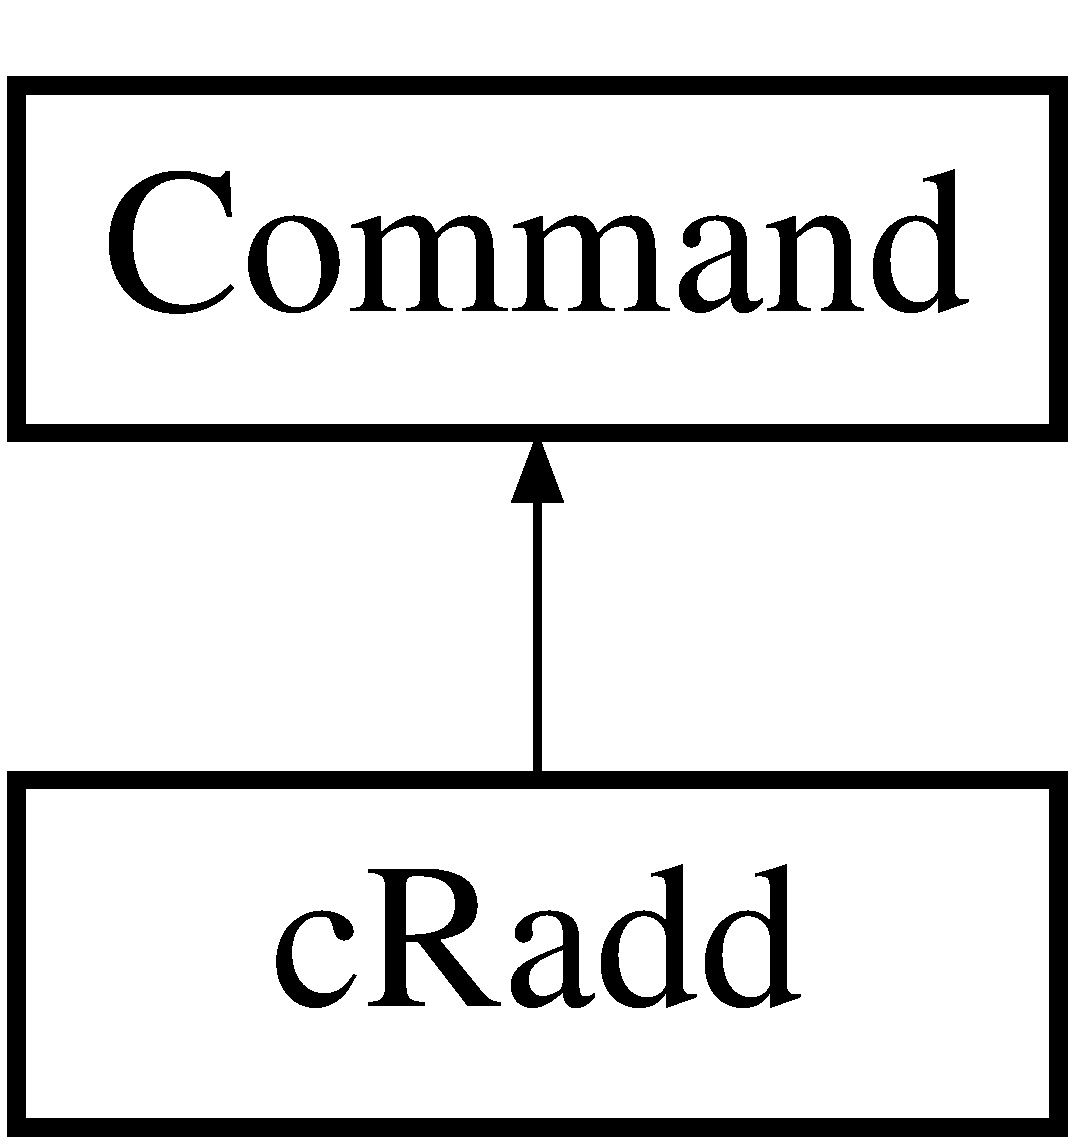
\includegraphics[height=2.000000cm]{classc_radd}
\end{center}
\end{figure}
\subsection*{Открытые члены}
\begin{DoxyCompactItemize}
\item 
int \hyperlink{classc_radd_a8a1aa83bf3a689bb0f547a9711b8b33a}{operator()} (\hyperlink{class_computer}{Computer} $\ast$C\+O\+MP)
\begin{DoxyCompactList}\small\item\em c\+Radd\+::operator () -\/ Вещественная сумма \end{DoxyCompactList}\end{DoxyCompactItemize}
\subsection*{Дополнительные унаследованные члены}


\subsection{Подробное описание}
Сложение дробных чисел 

\subsection{Методы}
\hypertarget{classc_radd_a8a1aa83bf3a689bb0f547a9711b8b33a}{}\label{classc_radd_a8a1aa83bf3a689bb0f547a9711b8b33a} 
\index{c\+Radd@{c\+Radd}!operator()@{operator()}}
\index{operator()@{operator()}!c\+Radd@{c\+Radd}}
\subsubsection{\texorpdfstring{operator()()}{operator()()}}
{\footnotesize\ttfamily int c\+Radd\+::operator() (\begin{DoxyParamCaption}\item[{\hyperlink{class_computer}{Computer} $\ast$}]{C\+O\+MP }\end{DoxyParamCaption})\hspace{0.3cm}{\ttfamily [virtual]}}



c\+Radd\+::operator () -\/ Вещественная сумма 


\begin{DoxyParams}{Аргументы}
{\em C\+O\+MP} & -\/ указатель на объект компьютер \\
\hline
\end{DoxyParams}
\begin{DoxyReturn}{Возвращает}
1
\end{DoxyReturn}
Загружает внутренний регистр по адресу. Складывает сумматор с внутренним регистром. Ставит флаги операции. 

Замещает \hyperlink{class_command_a79939b66f3de892e91d7710844294716}{Command}.


\begin{DoxyCode}
142 \{
143     \hyperlink{class_command_aac6f368e7c9dbb357b3f00627d5dabfc}{loadRegister}(COMP);
144     COMP->\hyperlink{class_computer_a874503110664b3cf821118d2ce9c2b96}{RS}.\hyperlink{union_computer_1_1data_acbf8c96e22bd094bcbb4014818e3570d}{R} += COMP->\hyperlink{class_computer_a0fbf84599b7db9d634a92afed443ee73}{R1}.\hyperlink{union_computer_1_1data_acbf8c96e22bd094bcbb4014818e3570d}{R};
145     COMP->\hyperlink{class_computer_aae860bb217270ec88e8ebf6fe2c2adc9}{flagR}(); \textcolor{comment}{//Установка флага результата}
146 
147     COMP->\hyperlink{class_computer_a10ca6c6b200630119201de16d7368e0f}{debug}(\textcolor{stringliteral}{"Вещественное сложение. Сумматор = "} + QString::number(COMP->
      \hyperlink{class_computer_a874503110664b3cf821118d2ce9c2b96}{RS}.\hyperlink{union_computer_1_1data_acbf8c96e22bd094bcbb4014818e3570d}{R}));
148     \textcolor{keywordflow}{return} 1;
149 \}
\end{DoxyCode}


Объявления и описания членов классов находятся в файлах\+:\begin{DoxyCompactItemize}
\item 
C\+:/\+Users/sstarkov/\+Documents/kr\+\_\+\+Interpreter\+V\+M/sources/command.\+h\item 
C\+:/\+Users/sstarkov/\+Documents/kr\+\_\+\+Interpreter\+V\+M/sources/command.\+cpp\end{DoxyCompactItemize}

\hypertarget{classc_radr}{}\section{Класс c\+Radr}
\label{classc_radr}\index{c\+Radr@{c\+Radr}}


Загрузка адрессного регистра  




{\ttfamily \#include $<$command.\+h$>$}

Граф наследования\+:c\+Radr\+:\begin{figure}[H]
\begin{center}
\leavevmode
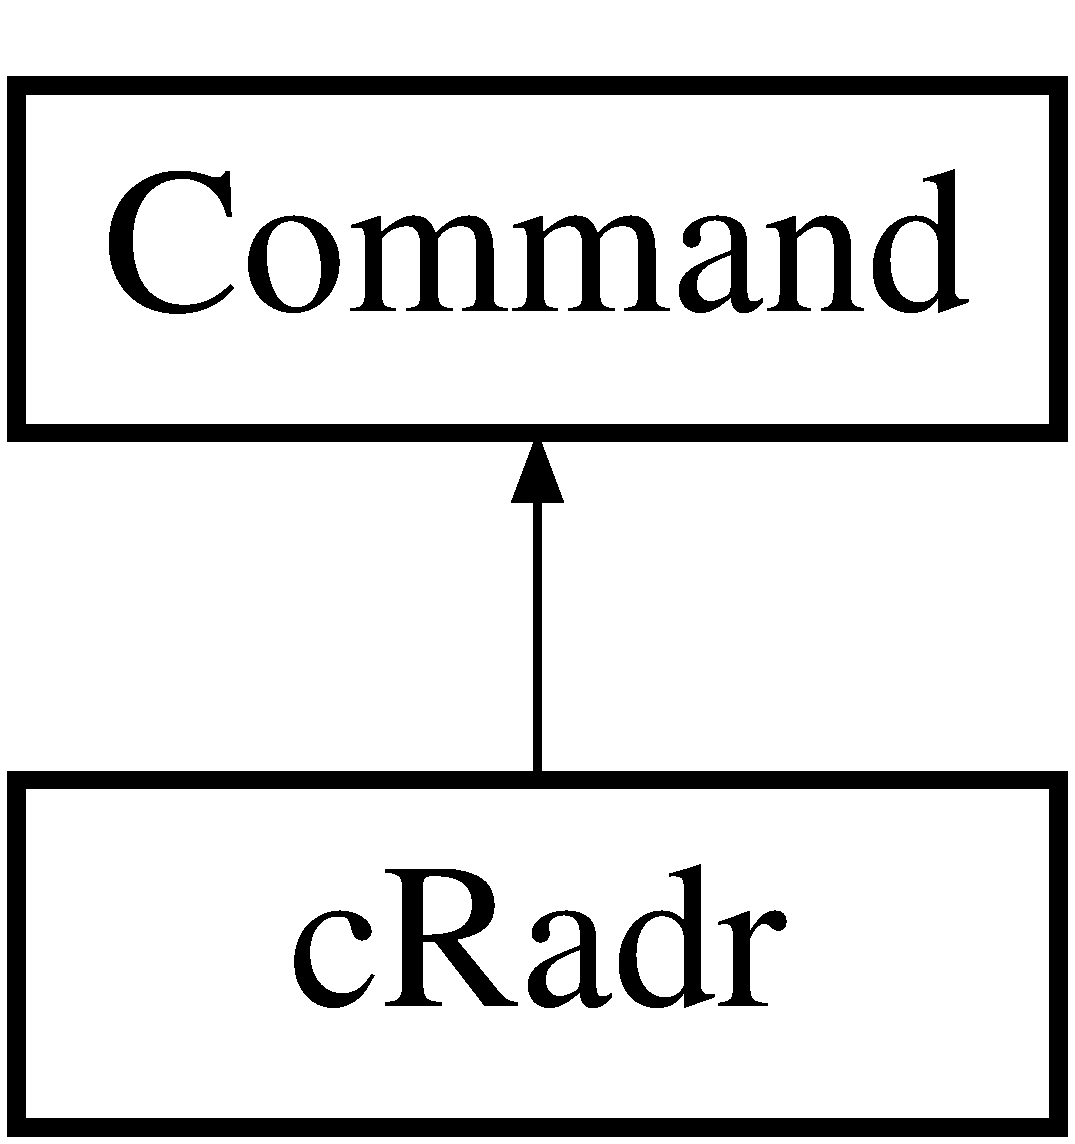
\includegraphics[height=2.000000cm]{classc_radr}
\end{center}
\end{figure}
\subsection*{Открытые члены}
\begin{DoxyCompactItemize}
\item 
int \hyperlink{classc_radr_af849046fb73e625b8c2c6380a70116f6}{operator()} (\hyperlink{class_computer}{Computer} $\ast$C\+O\+MP)
\begin{DoxyCompactList}\small\item\em c\+Radr\+::operator () -\/ Загрузка адресного регистра \end{DoxyCompactList}\end{DoxyCompactItemize}
\subsection*{Дополнительные унаследованные члены}


\subsection{Подробное описание}
Загрузка адрессного регистра 

\subsection{Методы}
\hypertarget{classc_radr_af849046fb73e625b8c2c6380a70116f6}{}\label{classc_radr_af849046fb73e625b8c2c6380a70116f6} 
\index{c\+Radr@{c\+Radr}!operator()@{operator()}}
\index{operator()@{operator()}!c\+Radr@{c\+Radr}}
\subsubsection{\texorpdfstring{operator()()}{operator()()}}
{\footnotesize\ttfamily int c\+Radr\+::operator() (\begin{DoxyParamCaption}\item[{\hyperlink{class_computer}{Computer} $\ast$}]{C\+O\+MP }\end{DoxyParamCaption})\hspace{0.3cm}{\ttfamily [virtual]}}



c\+Radr\+::operator () -\/ Загрузка адресного регистра 


\begin{DoxyParams}{Аргументы}
{\em C\+O\+MP} & -\/ указатель на объект компьютер \\
\hline
\end{DoxyParams}
\begin{DoxyReturn}{Возвращает}
1
\end{DoxyReturn}
Загружает в адресный регистр константу. Константа либо абсолютный адрес в ОЗУ, либо отступ от текущего значения адресного регистра. 

Замещает \hyperlink{class_command_a79939b66f3de892e91d7710844294716}{Command}.


\begin{DoxyCode}
269 \{
270     \textcolor{keywordflow}{if}(COMP->\hyperlink{class_computer_a8423168f7cc356b4dd36977603798caf}{CMD}.\hyperlink{struct_computer_1_1command_a3e0d1e527de9f60594023a362b08a7de}{B} == 0) \textcolor{comment}{//Абсолютная адресация}
271         COMP->\hyperlink{class_computer_a499d0b2c857c2977dd5702906705f79e}{RA} = COMP->\hyperlink{class_computer_a8423168f7cc356b4dd36977603798caf}{CMD}.\hyperlink{struct_computer_1_1command_a0e07591012953413797506f7bc3cb1a7}{Addr};
272     \textcolor{keywordflow}{else} \textcolor{comment}{//Относит адресация}
273         COMP->\hyperlink{class_computer_a499d0b2c857c2977dd5702906705f79e}{RA} += COMP->\hyperlink{class_computer_a8423168f7cc356b4dd36977603798caf}{CMD}.\hyperlink{struct_computer_1_1command_a0e07591012953413797506f7bc3cb1a7}{Addr};
274 
275     COMP->\hyperlink{class_computer_a10ca6c6b200630119201de16d7368e0f}{debug}(\textcolor{stringliteral}{"Установка адресного регистра на "} + QString::number(COMP->
      \hyperlink{class_computer_a499d0b2c857c2977dd5702906705f79e}{RA}));
276     \textcolor{keywordflow}{return} 1;
277 \}
\end{DoxyCode}


Объявления и описания членов классов находятся в файлах\+:\begin{DoxyCompactItemize}
\item 
C\+:/\+Users/sstarkov/\+Documents/kr\+\_\+\+Interpreter\+V\+M/sources/command.\+h\item 
C\+:/\+Users/sstarkov/\+Documents/kr\+\_\+\+Interpreter\+V\+M/sources/command.\+cpp\end{DoxyCompactItemize}

\hypertarget{classc_rcmp}{}\section{Класс c\+Rcmp}
\label{classc_rcmp}\index{c\+Rcmp@{c\+Rcmp}}


Сравнение вещественных  




{\ttfamily \#include $<$command.\+h$>$}

Граф наследования\+:c\+Rcmp\+:\begin{figure}[H]
\begin{center}
\leavevmode
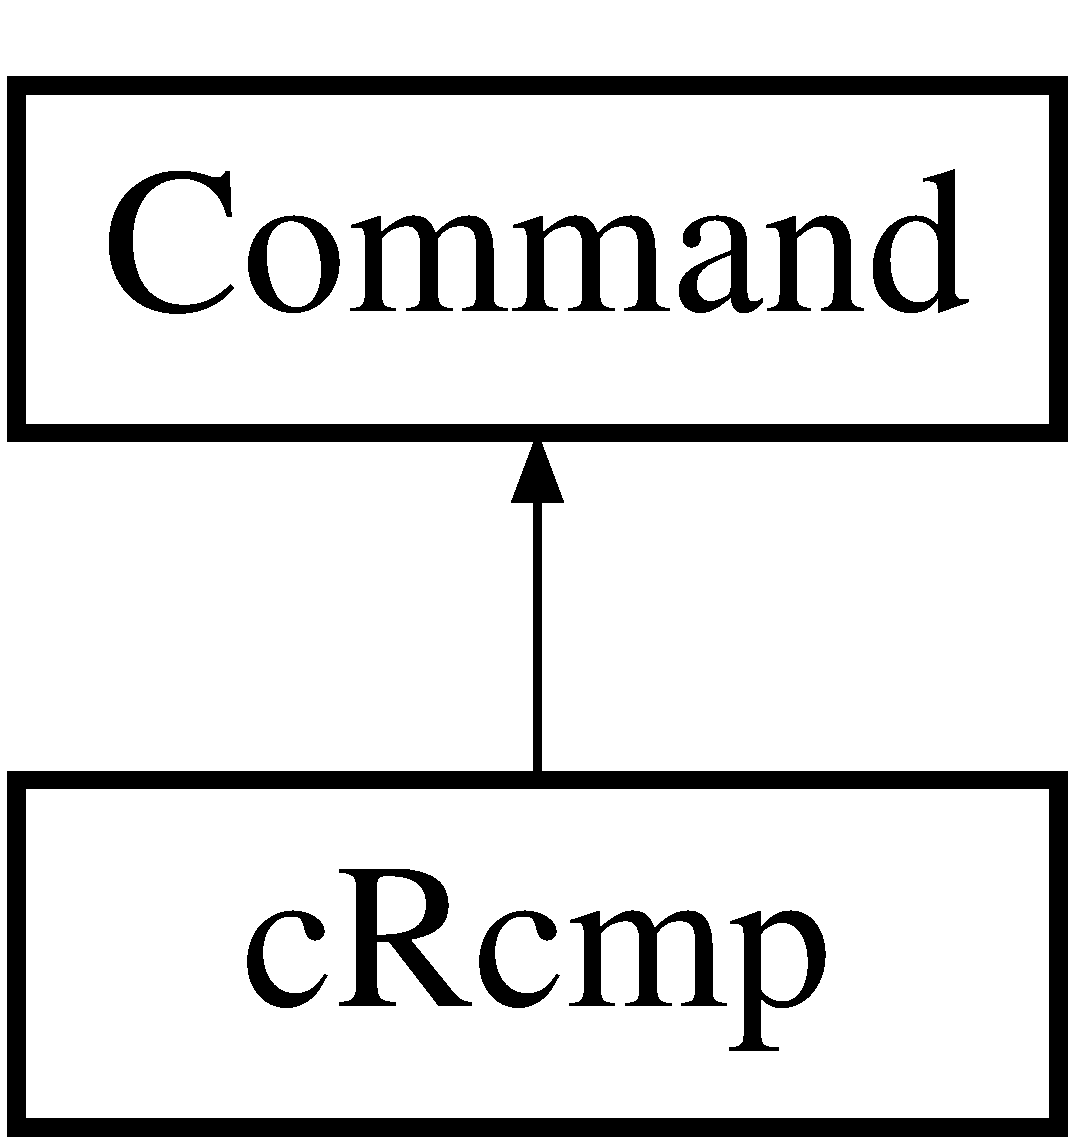
\includegraphics[height=2.000000cm]{classc_rcmp}
\end{center}
\end{figure}
\subsection*{Открытые члены}
\begin{DoxyCompactItemize}
\item 
int \hyperlink{classc_rcmp_a4053dd11e7f5f61ac61df639c425cf08}{operator()} (\hyperlink{class_computer}{Computer} $\ast$C\+O\+MP)
\begin{DoxyCompactList}\small\item\em c\+Rcmp\+::operator () -\/ Сравнение вещественных чисел \end{DoxyCompactList}\end{DoxyCompactItemize}
\subsection*{Дополнительные унаследованные члены}


\subsection{Подробное описание}
Сравнение вещественных 

\subsection{Методы}
\hypertarget{classc_rcmp_a4053dd11e7f5f61ac61df639c425cf08}{}\label{classc_rcmp_a4053dd11e7f5f61ac61df639c425cf08} 
\index{c\+Rcmp@{c\+Rcmp}!operator()@{operator()}}
\index{operator()@{operator()}!c\+Rcmp@{c\+Rcmp}}
\subsubsection{\texorpdfstring{operator()()}{operator()()}}
{\footnotesize\ttfamily int c\+Rcmp\+::operator() (\begin{DoxyParamCaption}\item[{\hyperlink{class_computer}{Computer} $\ast$}]{C\+O\+MP }\end{DoxyParamCaption})\hspace{0.3cm}{\ttfamily [virtual]}}



c\+Rcmp\+::operator () -\/ Сравнение вещественных чисел 


\begin{DoxyParams}{Аргументы}
{\em C\+O\+MP} & -\/ указатель на объект компьютер \\
\hline
\end{DoxyParams}
\begin{DoxyReturn}{Возвращает}
1
\end{DoxyReturn}
Загружает внутренний регистр из памяти. Сравнивает вещественное значение сумматора с вещественным значением внутреннего регистра. Результаты записываются в флаги P\+SW. Значение сумматора не изменяется. 

Замещает \hyperlink{class_command_a79939b66f3de892e91d7710844294716}{Command}.


\begin{DoxyCode}
312 \{
313     \hyperlink{class_command_aac6f368e7c9dbb357b3f00627d5dabfc}{loadRegister}(COMP);
314     COMP->\hyperlink{class_computer_adb154047da2156e4419af3b3a4a766b7}{DATA}.\hyperlink{union_computer_1_1data_acbf8c96e22bd094bcbb4014818e3570d}{R} = COMP->\hyperlink{class_computer_a874503110664b3cf821118d2ce9c2b96}{RS}.\hyperlink{union_computer_1_1data_acbf8c96e22bd094bcbb4014818e3570d}{R};
315     COMP->\hyperlink{class_computer_a874503110664b3cf821118d2ce9c2b96}{RS}.\hyperlink{union_computer_1_1data_acbf8c96e22bd094bcbb4014818e3570d}{R} -= COMP->\hyperlink{class_computer_a0fbf84599b7db9d634a92afed443ee73}{R1}.\hyperlink{union_computer_1_1data_acbf8c96e22bd094bcbb4014818e3570d}{R};
316     COMP->\hyperlink{class_computer_aae860bb217270ec88e8ebf6fe2c2adc9}{flagR}(); \textcolor{comment}{//Установка флага результата}
317     COMP->\hyperlink{class_computer_a874503110664b3cf821118d2ce9c2b96}{RS}.\hyperlink{union_computer_1_1data_acbf8c96e22bd094bcbb4014818e3570d}{R} = COMP->\hyperlink{class_computer_adb154047da2156e4419af3b3a4a766b7}{DATA}.\hyperlink{union_computer_1_1data_acbf8c96e22bd094bcbb4014818e3570d}{R};
318 
319     COMP->\hyperlink{class_computer_a10ca6c6b200630119201de16d7368e0f}{debug}(\textcolor{stringliteral}{"Вещественное сравнение"});
320     \textcolor{keywordflow}{return} 1;
321 \}
\end{DoxyCode}


Объявления и описания членов классов находятся в файлах\+:\begin{DoxyCompactItemize}
\item 
C\+:/\+Users/sstarkov/\+Documents/kr\+\_\+\+Interpreter\+V\+M/sources/command.\+h\item 
C\+:/\+Users/sstarkov/\+Documents/kr\+\_\+\+Interpreter\+V\+M/sources/command.\+cpp\end{DoxyCompactItemize}

\hypertarget{classc_rdiv}{}\section{Класс c\+Rdiv}
\label{classc_rdiv}\index{c\+Rdiv@{c\+Rdiv}}


Деление дробных чисел  




{\ttfamily \#include $<$command.\+h$>$}

Граф наследования\+:c\+Rdiv\+:\begin{figure}[H]
\begin{center}
\leavevmode
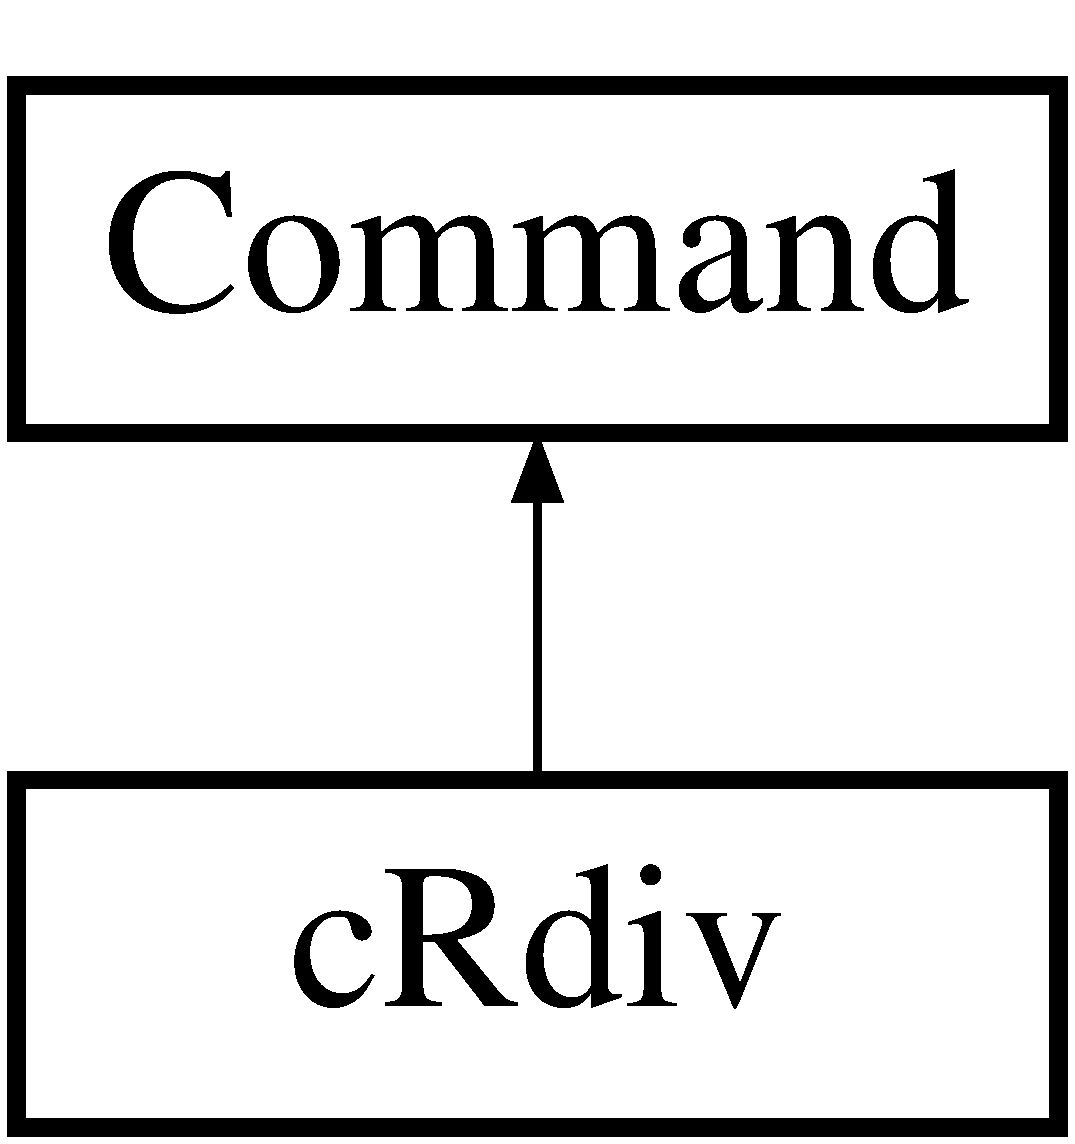
\includegraphics[height=2.000000cm]{classc_rdiv}
\end{center}
\end{figure}
\subsection*{Открытые члены}
\begin{DoxyCompactItemize}
\item 
int \hyperlink{classc_rdiv_a2ce07afa960d74895bcfc2028220e51b}{operator()} (\hyperlink{class_computer}{Computer} $\ast$C\+O\+MP)
\begin{DoxyCompactList}\small\item\em c\+Rdiv\+::operator () -\/ вещественное деление \end{DoxyCompactList}\end{DoxyCompactItemize}
\subsection*{Дополнительные унаследованные члены}


\subsection{Подробное описание}
Деление дробных чисел 

\subsection{Методы}
\hypertarget{classc_rdiv_a2ce07afa960d74895bcfc2028220e51b}{}\label{classc_rdiv_a2ce07afa960d74895bcfc2028220e51b} 
\index{c\+Rdiv@{c\+Rdiv}!operator()@{operator()}}
\index{operator()@{operator()}!c\+Rdiv@{c\+Rdiv}}
\subsubsection{\texorpdfstring{operator()()}{operator()()}}
{\footnotesize\ttfamily int c\+Rdiv\+::operator() (\begin{DoxyParamCaption}\item[{\hyperlink{class_computer}{Computer} $\ast$}]{C\+O\+MP }\end{DoxyParamCaption})\hspace{0.3cm}{\ttfamily [virtual]}}



c\+Rdiv\+::operator () -\/ вещественное деление 


\begin{DoxyParams}{Аргументы}
{\em C\+O\+MP} & -\/ указатель на объект компьютер \\
\hline
\end{DoxyParams}
\begin{DoxyReturn}{Возвращает}
1
\end{DoxyReturn}
Загружает внутренний регистр по адресу. Делит сумматор на значение внутреннего регистра. Ставит флаги операции. 

Замещает \hyperlink{class_command_a79939b66f3de892e91d7710844294716}{Command}.


\begin{DoxyCode}
199 \{
200     \hyperlink{class_command_aac6f368e7c9dbb357b3f00627d5dabfc}{loadRegister}(COMP);
201     COMP->\hyperlink{class_computer_a874503110664b3cf821118d2ce9c2b96}{RS}.\hyperlink{union_computer_1_1data_acbf8c96e22bd094bcbb4014818e3570d}{R} /= COMP->\hyperlink{class_computer_a0fbf84599b7db9d634a92afed443ee73}{R1}.\hyperlink{union_computer_1_1data_acbf8c96e22bd094bcbb4014818e3570d}{R};
202     COMP->\hyperlink{class_computer_aae860bb217270ec88e8ebf6fe2c2adc9}{flagR}(); \textcolor{comment}{//Установка флага результата}
203 
204     COMP->\hyperlink{class_computer_a10ca6c6b200630119201de16d7368e0f}{debug}(\textcolor{stringliteral}{"Вещественное деление. Сумматор = "} + QString::number(COMP->
      \hyperlink{class_computer_a874503110664b3cf821118d2ce9c2b96}{RS}.\hyperlink{union_computer_1_1data_acbf8c96e22bd094bcbb4014818e3570d}{R}));
205     \textcolor{keywordflow}{return} 1;
206 \}
\end{DoxyCode}


Объявления и описания членов классов находятся в файлах\+:\begin{DoxyCompactItemize}
\item 
C\+:/\+Users/sstarkov/\+Documents/kr\+\_\+\+Interpreter\+V\+M/sources/command.\+h\item 
C\+:/\+Users/sstarkov/\+Documents/kr\+\_\+\+Interpreter\+V\+M/sources/command.\+cpp\end{DoxyCompactItemize}

\hypertarget{classc_rin}{}\section{Класс c\+Rin}
\label{classc_rin}\index{c\+Rin@{c\+Rin}}


Ввод вещественного  




{\ttfamily \#include $<$command.\+h$>$}

Граф наследования\+:c\+Rin\+:\begin{figure}[H]
\begin{center}
\leavevmode
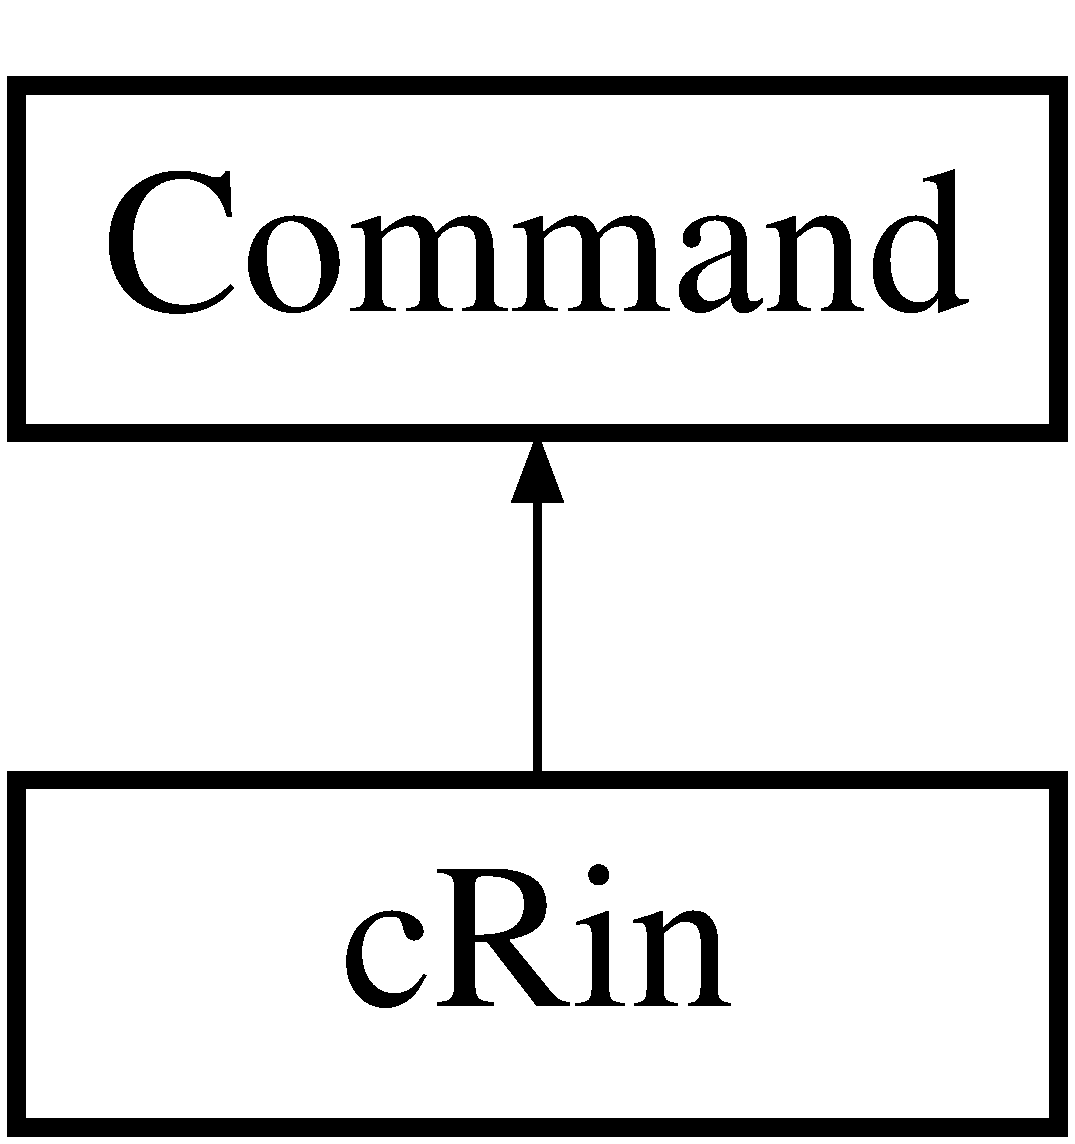
\includegraphics[height=2.000000cm]{classc_rin}
\end{center}
\end{figure}
\subsection*{Открытые члены}
\begin{DoxyCompactItemize}
\item 
int \hyperlink{classc_rin_a28177e2dd8dcc938881ff6629ecd5685}{operator()} (\hyperlink{class_computer}{Computer} $\ast$C\+O\+MP)
\begin{DoxyCompactList}\small\item\em c\+Rin\+::operator () -\/ Прерывание\+: ввод вещественного значения \end{DoxyCompactList}\end{DoxyCompactItemize}
\subsection*{Дополнительные унаследованные члены}


\subsection{Подробное описание}
Ввод вещественного 

\subsection{Методы}
\hypertarget{classc_rin_a28177e2dd8dcc938881ff6629ecd5685}{}\label{classc_rin_a28177e2dd8dcc938881ff6629ecd5685} 
\index{c\+Rin@{c\+Rin}!operator()@{operator()}}
\index{operator()@{operator()}!c\+Rin@{c\+Rin}}
\subsubsection{\texorpdfstring{operator()()}{operator()()}}
{\footnotesize\ttfamily int c\+Rin\+::operator() (\begin{DoxyParamCaption}\item[{\hyperlink{class_computer}{Computer} $\ast$}]{C\+O\+MP }\end{DoxyParamCaption})\hspace{0.3cm}{\ttfamily [virtual]}}



c\+Rin\+::operator () -\/ Прерывание\+: ввод вещественного значения 


\begin{DoxyParams}{Аргументы}
{\em C\+O\+MP} & -\/ указатель на объект компьютер \\
\hline
\end{DoxyParams}
\begin{DoxyReturn}{Возвращает}
1
\end{DoxyReturn}
Вызывает прерывание для ввода Вещественного значения от пользователя и загружает его в сумматор 

Замещает \hyperlink{class_command_a79939b66f3de892e91d7710844294716}{Command}.


\begin{DoxyCode}
425 \{
426     COMP->\hyperlink{class_computer_aa57b0ed2f3a9b168c2924174ec524bd4}{interrupt}(hRin);
427     COMP->\hyperlink{class_computer_a874503110664b3cf821118d2ce9c2b96}{RS}.\hyperlink{union_computer_1_1data_acbf8c96e22bd094bcbb4014818e3570d}{R} = COMP->\hyperlink{class_computer_adb154047da2156e4419af3b3a4a766b7}{DATA}.\hyperlink{union_computer_1_1data_acbf8c96e22bd094bcbb4014818e3570d}{R};
428 
429     COMP->\hyperlink{class_computer_a10ca6c6b200630119201de16d7368e0f}{debug}(\textcolor{stringliteral}{"Ввод вещественного числа "} + QString::number(COMP->\hyperlink{class_computer_a874503110664b3cf821118d2ce9c2b96}{RS}.\hyperlink{union_computer_1_1data_acbf8c96e22bd094bcbb4014818e3570d}{R}));
430     \textcolor{keywordflow}{return} 1;
431 \}
\end{DoxyCode}


Объявления и описания членов классов находятся в файлах\+:\begin{DoxyCompactItemize}
\item 
C\+:/\+Users/sstarkov/\+Documents/kr\+\_\+\+Interpreter\+V\+M/sources/command.\+h\item 
C\+:/\+Users/sstarkov/\+Documents/kr\+\_\+\+Interpreter\+V\+M/sources/command.\+cpp\end{DoxyCompactItemize}

\hypertarget{classc_rmul}{}\section{Класс c\+Rmul}
\label{classc_rmul}\index{c\+Rmul@{c\+Rmul}}


Умножение дробных чисел  




{\ttfamily \#include $<$command.\+h$>$}

Граф наследования\+:c\+Rmul\+:\begin{figure}[H]
\begin{center}
\leavevmode
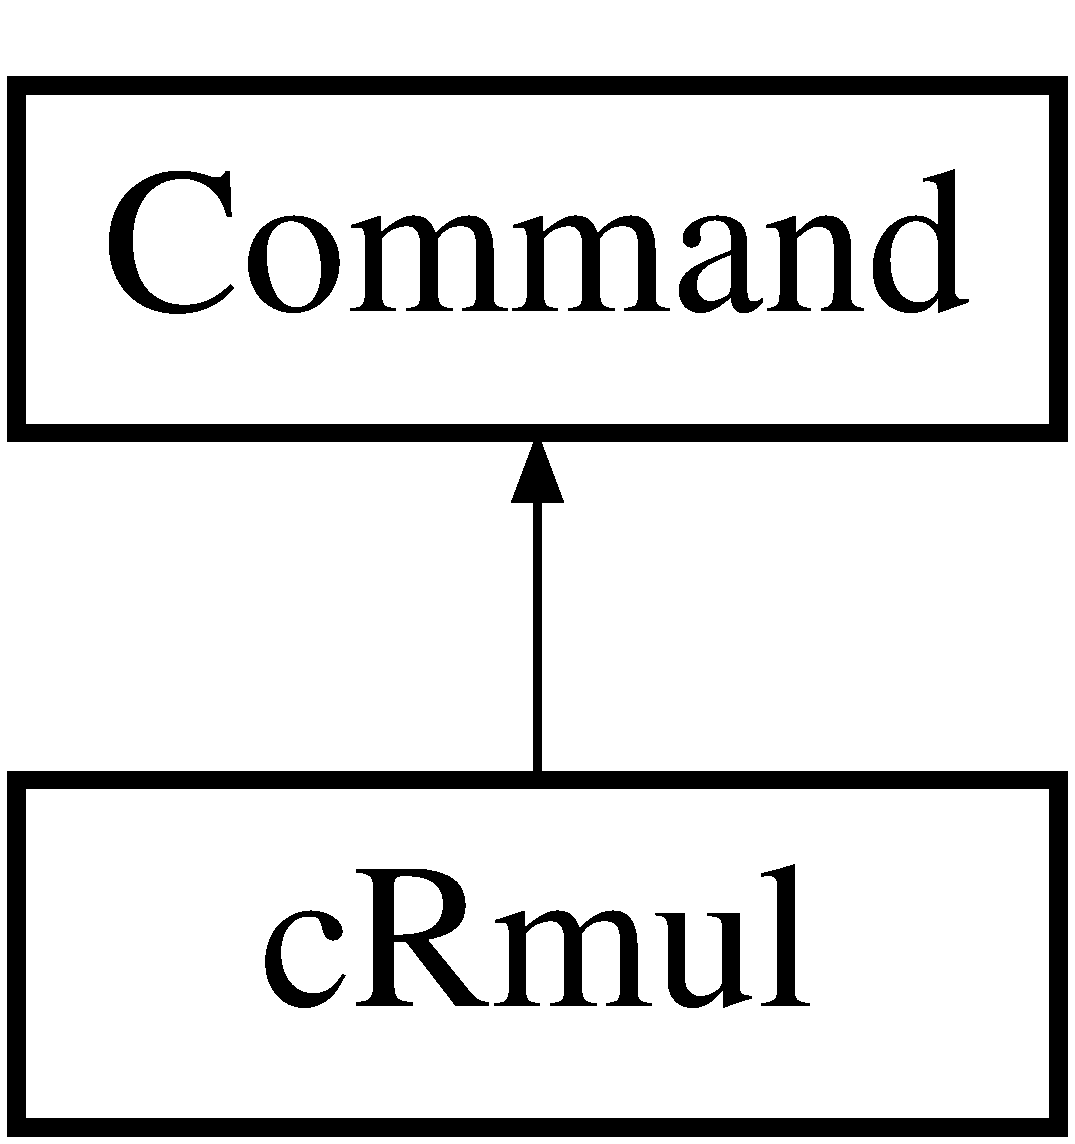
\includegraphics[height=2.000000cm]{classc_rmul}
\end{center}
\end{figure}
\subsection*{Открытые члены}
\begin{DoxyCompactItemize}
\item 
int \hyperlink{classc_rmul_a59cc32a7f9833fd05fe1c8f9e60f48b3}{operator()} (\hyperlink{class_computer}{Computer} $\ast$C\+O\+MP)
\begin{DoxyCompactList}\small\item\em c\+Rmul\+::operator () -\/ Вещественное произведение \end{DoxyCompactList}\end{DoxyCompactItemize}
\subsection*{Дополнительные унаследованные члены}


\subsection{Подробное описание}
Умножение дробных чисел 

\subsection{Методы}
\hypertarget{classc_rmul_a59cc32a7f9833fd05fe1c8f9e60f48b3}{}\label{classc_rmul_a59cc32a7f9833fd05fe1c8f9e60f48b3} 
\index{c\+Rmul@{c\+Rmul}!operator()@{operator()}}
\index{operator()@{operator()}!c\+Rmul@{c\+Rmul}}
\subsubsection{\texorpdfstring{operator()()}{operator()()}}
{\footnotesize\ttfamily int c\+Rmul\+::operator() (\begin{DoxyParamCaption}\item[{\hyperlink{class_computer}{Computer} $\ast$}]{C\+O\+MP }\end{DoxyParamCaption})\hspace{0.3cm}{\ttfamily [virtual]}}



c\+Rmul\+::operator () -\/ Вещественное произведение 


\begin{DoxyParams}{Аргументы}
{\em C\+O\+MP} & -\/ указатель на объект компьютер \\
\hline
\end{DoxyParams}
\begin{DoxyReturn}{Возвращает}
1
\end{DoxyReturn}
Загружает внутренний регистр по адресу. Умножает сумматор на внутренний регистр Ставит флаги операции. 

Замещает \hyperlink{class_command_a79939b66f3de892e91d7710844294716}{Command}.


\begin{DoxyCode}
180 \{
181     \hyperlink{class_command_aac6f368e7c9dbb357b3f00627d5dabfc}{loadRegister}(COMP);
182     COMP->\hyperlink{class_computer_a874503110664b3cf821118d2ce9c2b96}{RS}.\hyperlink{union_computer_1_1data_acbf8c96e22bd094bcbb4014818e3570d}{R} *= COMP->\hyperlink{class_computer_a0fbf84599b7db9d634a92afed443ee73}{R1}.\hyperlink{union_computer_1_1data_acbf8c96e22bd094bcbb4014818e3570d}{R};
183     COMP->\hyperlink{class_computer_aae860bb217270ec88e8ebf6fe2c2adc9}{flagR}(); \textcolor{comment}{//Установка флага результата}
184 
185     COMP->\hyperlink{class_computer_a10ca6c6b200630119201de16d7368e0f}{debug}(\textcolor{stringliteral}{"Вещественное умножение. Сумматор = "} + QString::number(COMP->
      \hyperlink{class_computer_a874503110664b3cf821118d2ce9c2b96}{RS}.\hyperlink{union_computer_1_1data_acbf8c96e22bd094bcbb4014818e3570d}{R}));
186     \textcolor{keywordflow}{return} 1;
187 \}
\end{DoxyCode}


Объявления и описания членов классов находятся в файлах\+:\begin{DoxyCompactItemize}
\item 
C\+:/\+Users/sstarkov/\+Documents/kr\+\_\+\+Interpreter\+V\+M/sources/command.\+h\item 
C\+:/\+Users/sstarkov/\+Documents/kr\+\_\+\+Interpreter\+V\+M/sources/command.\+cpp\end{DoxyCompactItemize}

\hypertarget{classc_rout}{}\section{Класс c\+Rout}
\label{classc_rout}\index{c\+Rout@{c\+Rout}}


Вывод вещественного  




{\ttfamily \#include $<$command.\+h$>$}

Граф наследования\+:c\+Rout\+:\begin{figure}[H]
\begin{center}
\leavevmode
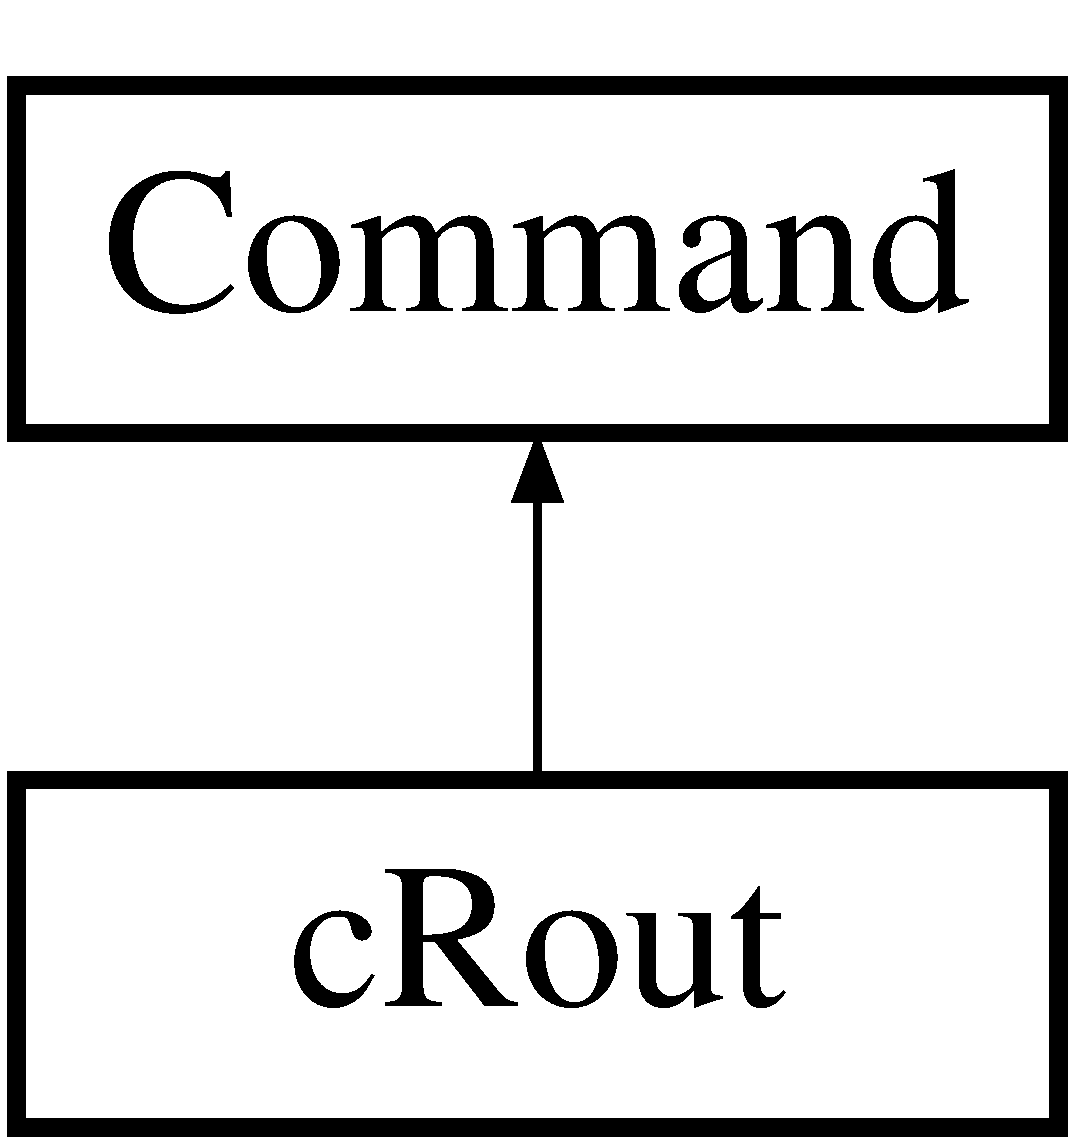
\includegraphics[height=2.000000cm]{classc_rout}
\end{center}
\end{figure}
\subsection*{Открытые члены}
\begin{DoxyCompactItemize}
\item 
int \hyperlink{classc_rout_a25d1eb608870665eccbf6beb529d8999}{operator()} (\hyperlink{class_computer}{Computer} $\ast$C\+O\+MP)
\begin{DoxyCompactList}\small\item\em c\+Rout\+::operator () -\/ Прерывание\+: вывод вещественного значения из сумматора \end{DoxyCompactList}\end{DoxyCompactItemize}
\subsection*{Дополнительные унаследованные члены}


\subsection{Подробное описание}
Вывод вещественного 

\subsection{Методы}
\hypertarget{classc_rout_a25d1eb608870665eccbf6beb529d8999}{}\label{classc_rout_a25d1eb608870665eccbf6beb529d8999} 
\index{c\+Rout@{c\+Rout}!operator()@{operator()}}
\index{operator()@{operator()}!c\+Rout@{c\+Rout}}
\subsubsection{\texorpdfstring{operator()()}{operator()()}}
{\footnotesize\ttfamily int c\+Rout\+::operator() (\begin{DoxyParamCaption}\item[{\hyperlink{class_computer}{Computer} $\ast$}]{C\+O\+MP }\end{DoxyParamCaption})\hspace{0.3cm}{\ttfamily [virtual]}}



c\+Rout\+::operator () -\/ Прерывание\+: вывод вещественного значения из сумматора 


\begin{DoxyParams}{Аргументы}
{\em C\+O\+MP} & -\/ указатель на объект компьютер \\
\hline
\end{DoxyParams}
\begin{DoxyReturn}{Возвращает}
1
\end{DoxyReturn}
Вызывает прерывание для вывода вещественного значения на экран 

Замещает \hyperlink{class_command_a79939b66f3de892e91d7710844294716}{Command}.


\begin{DoxyCode}
455 \{
456     COMP->\hyperlink{class_computer_a10ca6c6b200630119201de16d7368e0f}{debug}(\textcolor{stringliteral}{"Вывод вещественного числа "} + QString::number(COMP->\hyperlink{class_computer_a874503110664b3cf821118d2ce9c2b96}{RS}.\hyperlink{union_computer_1_1data_acbf8c96e22bd094bcbb4014818e3570d}{R}));
457     COMP->\hyperlink{class_computer_aa57b0ed2f3a9b168c2924174ec524bd4}{interrupt}(hRout);
458     \textcolor{keywordflow}{return} 1;
459 \}
\end{DoxyCode}


Объявления и описания членов классов находятся в файлах\+:\begin{DoxyCompactItemize}
\item 
C\+:/\+Users/sstarkov/\+Documents/kr\+\_\+\+Interpreter\+V\+M/sources/command.\+h\item 
C\+:/\+Users/sstarkov/\+Documents/kr\+\_\+\+Interpreter\+V\+M/sources/command.\+cpp\end{DoxyCompactItemize}

\hypertarget{classc_rsub}{}\section{Класс c\+Rsub}
\label{classc_rsub}\index{c\+Rsub@{c\+Rsub}}


Вычитание дробных чисел  




{\ttfamily \#include $<$command.\+h$>$}

Граф наследования\+:c\+Rsub\+:\begin{figure}[H]
\begin{center}
\leavevmode
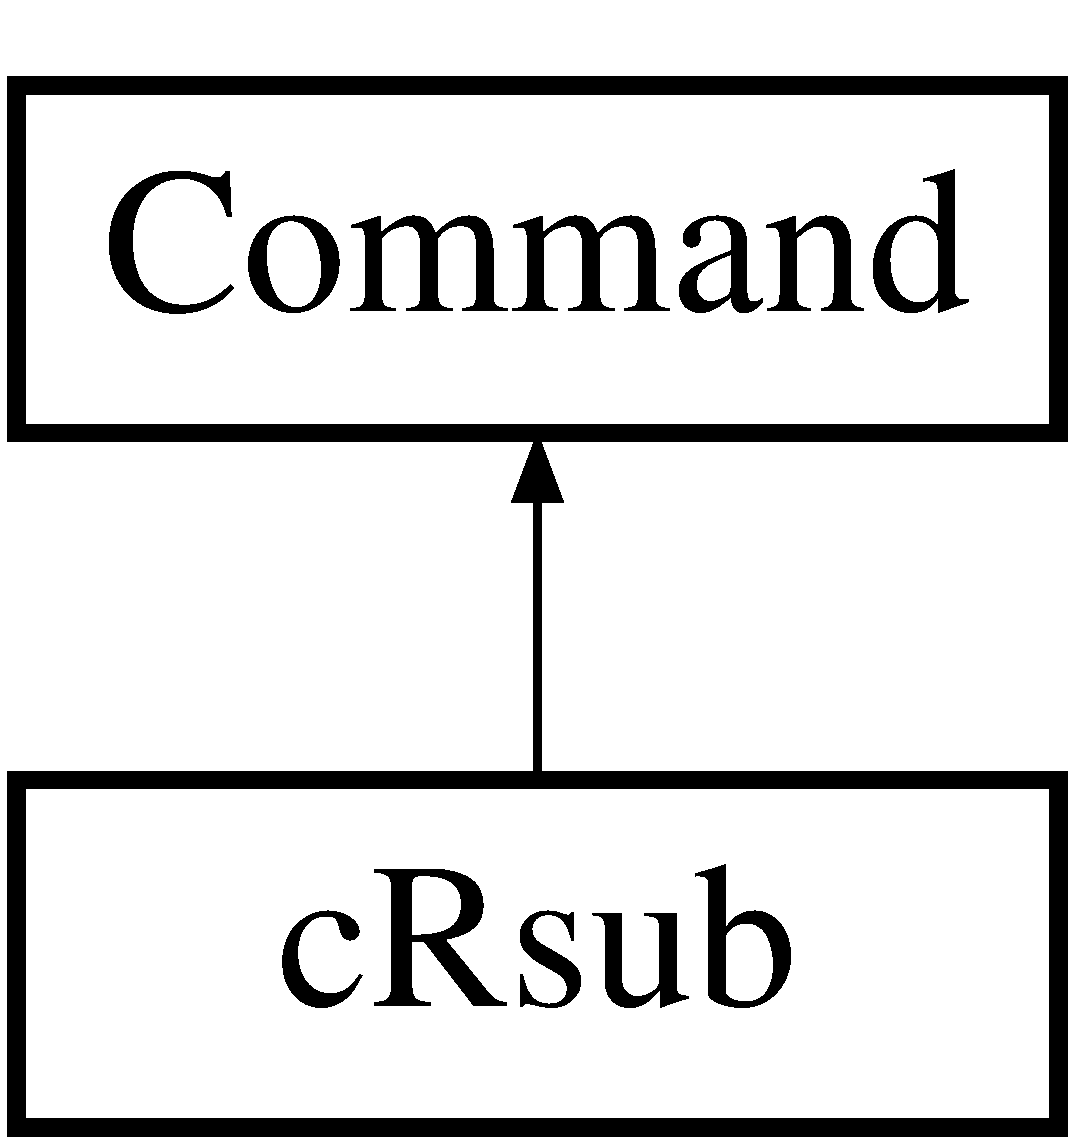
\includegraphics[height=2.000000cm]{classc_rsub}
\end{center}
\end{figure}
\subsection*{Открытые члены}
\begin{DoxyCompactItemize}
\item 
int \hyperlink{classc_rsub_a270572d89750986cbb1258f765965875}{operator()} (\hyperlink{class_computer}{Computer} $\ast$C\+O\+MP)
\begin{DoxyCompactList}\small\item\em c\+Rsub\+::operator () -\/ Вещественная разность \end{DoxyCompactList}\end{DoxyCompactItemize}
\subsection*{Дополнительные унаследованные члены}


\subsection{Подробное описание}
Вычитание дробных чисел 

\subsection{Методы}
\hypertarget{classc_rsub_a270572d89750986cbb1258f765965875}{}\label{classc_rsub_a270572d89750986cbb1258f765965875} 
\index{c\+Rsub@{c\+Rsub}!operator()@{operator()}}
\index{operator()@{operator()}!c\+Rsub@{c\+Rsub}}
\subsubsection{\texorpdfstring{operator()()}{operator()()}}
{\footnotesize\ttfamily int c\+Rsub\+::operator() (\begin{DoxyParamCaption}\item[{\hyperlink{class_computer}{Computer} $\ast$}]{C\+O\+MP }\end{DoxyParamCaption})\hspace{0.3cm}{\ttfamily [virtual]}}



c\+Rsub\+::operator () -\/ Вещественная разность 


\begin{DoxyParams}{Аргументы}
{\em C\+O\+MP} & -\/ указатель на объект компьютер \\
\hline
\end{DoxyParams}
\begin{DoxyReturn}{Возвращает}
1
\end{DoxyReturn}
Загружает внутренний регистр по адресу. Вичитает из сумматора значение внутреннего регистра. Ставит флаги операции. 

Замещает \hyperlink{class_command_a79939b66f3de892e91d7710844294716}{Command}.


\begin{DoxyCode}
161 \{
162     \hyperlink{class_command_aac6f368e7c9dbb357b3f00627d5dabfc}{loadRegister}(COMP);
163     COMP->\hyperlink{class_computer_a874503110664b3cf821118d2ce9c2b96}{RS}.\hyperlink{union_computer_1_1data_acbf8c96e22bd094bcbb4014818e3570d}{R} -= COMP->\hyperlink{class_computer_a0fbf84599b7db9d634a92afed443ee73}{R1}.\hyperlink{union_computer_1_1data_acbf8c96e22bd094bcbb4014818e3570d}{R};
164     COMP->\hyperlink{class_computer_aae860bb217270ec88e8ebf6fe2c2adc9}{flagR}(); \textcolor{comment}{//Установка флага результата}
165 
166     COMP->\hyperlink{class_computer_a10ca6c6b200630119201de16d7368e0f}{debug}(\textcolor{stringliteral}{"Вещественное вычитание. Сумматор = "} + QString::number(COMP->
      \hyperlink{class_computer_a874503110664b3cf821118d2ce9c2b96}{RS}.\hyperlink{union_computer_1_1data_acbf8c96e22bd094bcbb4014818e3570d}{R}));
167     \textcolor{keywordflow}{return} 1;
168 \}
\end{DoxyCode}


Объявления и описания членов классов находятся в файлах\+:\begin{DoxyCompactItemize}
\item 
C\+:/\+Users/sstarkov/\+Documents/kr\+\_\+\+Interpreter\+V\+M/sources/command.\+h\item 
C\+:/\+Users/sstarkov/\+Documents/kr\+\_\+\+Interpreter\+V\+M/sources/command.\+cpp\end{DoxyCompactItemize}

\hypertarget{classc_s_t_o_p}{}\section{Класс c\+S\+T\+OP}
\label{classc_s_t_o_p}\index{c\+S\+T\+OP@{c\+S\+T\+OP}}


СТОП  




{\ttfamily \#include $<$command.\+h$>$}

Граф наследования\+:c\+S\+T\+OP\+:\begin{figure}[H]
\begin{center}
\leavevmode
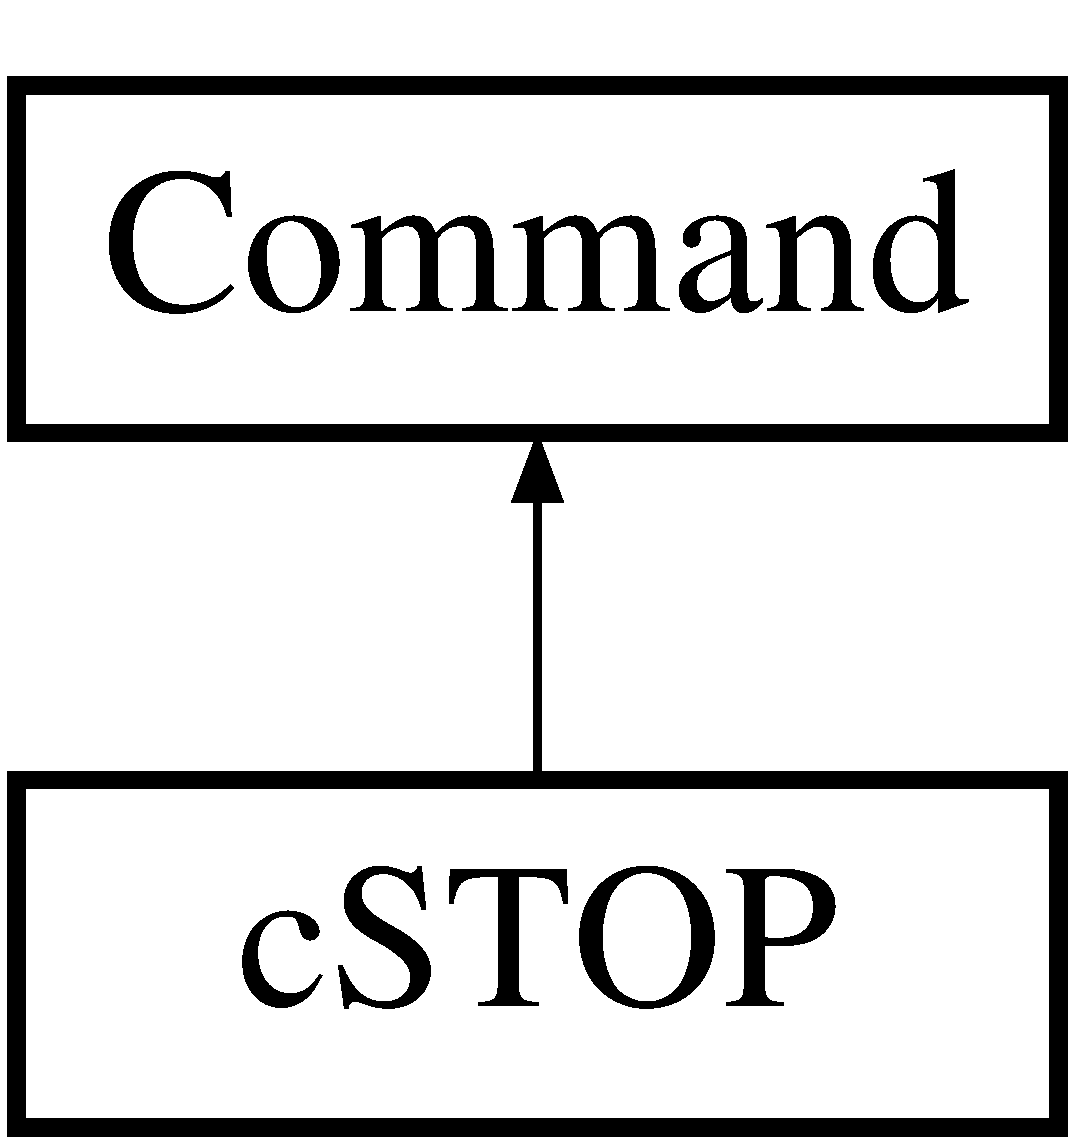
\includegraphics[height=2.000000cm]{classc_s_t_o_p}
\end{center}
\end{figure}
\subsection*{Открытые члены}
\begin{DoxyCompactItemize}
\item 
int \hyperlink{classc_s_t_o_p_ab9fc397331682767a4429257cdd14695}{operator()} (\hyperlink{class_computer}{Computer} $\ast$)
\begin{DoxyCompactList}\small\item\em c\+S\+T\+O\+P\+::operator () \end{DoxyCompactList}\end{DoxyCompactItemize}
\subsection*{Дополнительные унаследованные члены}


\subsection{Подробное описание}
СТОП 

\subsection{Методы}
\hypertarget{classc_s_t_o_p_ab9fc397331682767a4429257cdd14695}{}\label{classc_s_t_o_p_ab9fc397331682767a4429257cdd14695} 
\index{c\+S\+T\+OP@{c\+S\+T\+OP}!operator()@{operator()}}
\index{operator()@{operator()}!c\+S\+T\+OP@{c\+S\+T\+OP}}
\subsubsection{\texorpdfstring{operator()()}{operator()()}}
{\footnotesize\ttfamily int c\+S\+T\+O\+P\+::operator() (\begin{DoxyParamCaption}\item[{\hyperlink{class_computer}{Computer} $\ast$}]{ }\end{DoxyParamCaption})\hspace{0.3cm}{\ttfamily [virtual]}}



c\+S\+T\+O\+P\+::operator () 

\begin{DoxyReturn}{Возвращает}
0
\end{DoxyReturn}
Завершает работу программы 

Замещает \hyperlink{class_command_a79939b66f3de892e91d7710844294716}{Command}.


\begin{DoxyCode}
33 \{
34     \textcolor{keywordflow}{return} 0;
35 \}
\end{DoxyCode}


Объявления и описания членов классов находятся в файлах\+:\begin{DoxyCompactItemize}
\item 
C\+:/\+Users/sstarkov/\+Documents/kr\+\_\+\+Interpreter\+V\+M/sources/command.\+h\item 
C\+:/\+Users/sstarkov/\+Documents/kr\+\_\+\+Interpreter\+V\+M/sources/command.\+cpp\end{DoxyCompactItemize}

\hypertarget{classc_store}{}\section{Класс c\+Store}
\label{classc_store}\index{c\+Store@{c\+Store}}


Выгрузка сумматора  




{\ttfamily \#include $<$command.\+h$>$}

Граф наследования\+:c\+Store\+:\begin{figure}[H]
\begin{center}
\leavevmode
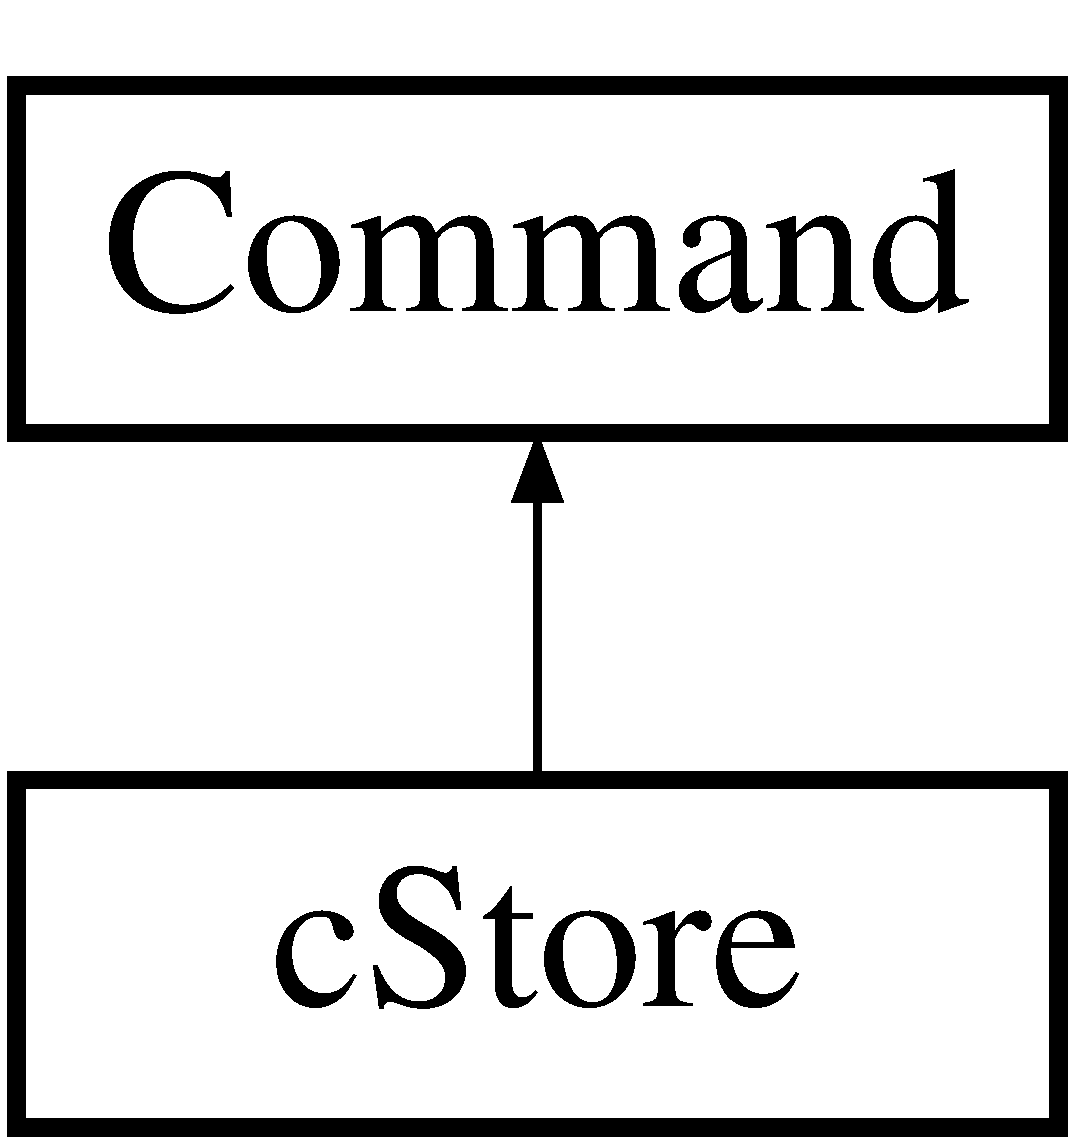
\includegraphics[height=2.000000cm]{classc_store}
\end{center}
\end{figure}
\subsection*{Открытые члены}
\begin{DoxyCompactItemize}
\item 
int \hyperlink{classc_store_a4822a996170072d5c9befde5281b6276}{operator()} (\hyperlink{class_computer}{Computer} $\ast$C\+O\+MP)
\begin{DoxyCompactList}\small\item\em c\+Store\+::operator () -\/ Выгрузка сумматора \end{DoxyCompactList}\end{DoxyCompactItemize}
\subsection*{Дополнительные унаследованные члены}


\subsection{Подробное описание}
Выгрузка сумматора 

\subsection{Методы}
\hypertarget{classc_store_a4822a996170072d5c9befde5281b6276}{}\label{classc_store_a4822a996170072d5c9befde5281b6276} 
\index{c\+Store@{c\+Store}!operator()@{operator()}}
\index{operator()@{operator()}!c\+Store@{c\+Store}}
\subsubsection{\texorpdfstring{operator()()}{operator()()}}
{\footnotesize\ttfamily int c\+Store\+::operator() (\begin{DoxyParamCaption}\item[{\hyperlink{class_computer}{Computer} $\ast$}]{C\+O\+MP }\end{DoxyParamCaption})\hspace{0.3cm}{\ttfamily [virtual]}}



c\+Store\+::operator () -\/ Выгрузка сумматора 


\begin{DoxyParams}{Аргументы}
{\em C\+O\+MP} & -\/ указатель на объект компьютер \\
\hline
\end{DoxyParams}
\begin{DoxyReturn}{Возвращает}
1
\end{DoxyReturn}
Выгружает сумматор в оперативную память. Размер выгрузки 4 байта. 

Замещает \hyperlink{class_command_a79939b66f3de892e91d7710844294716}{Command}.


\begin{DoxyCode}
243 \{
244     address ptr;
245     \textcolor{keywordflow}{if}(COMP->\hyperlink{class_computer_a8423168f7cc356b4dd36977603798caf}{CMD}.\hyperlink{struct_computer_1_1command_a3e0d1e527de9f60594023a362b08a7de}{B} == 0) \textcolor{comment}{//Абсолютная адресация}
246         ptr =  COMP->\hyperlink{class_computer_a8423168f7cc356b4dd36977603798caf}{CMD}.\hyperlink{struct_computer_1_1command_a0e07591012953413797506f7bc3cb1a7}{Addr};
247     \textcolor{keywordflow}{else} \textcolor{comment}{//Относит адресация}
248         ptr = COMP->\hyperlink{class_computer_a8423168f7cc356b4dd36977603798caf}{CMD}.\hyperlink{struct_computer_1_1command_a0e07591012953413797506f7bc3cb1a7}{Addr} + COMP->\hyperlink{class_computer_a499d0b2c857c2977dd5702906705f79e}{RA};
249 
250     COMP->\hyperlink{class_computer_a10ca6c6b200630119201de16d7368e0f}{debug}(\textcolor{stringliteral}{"Выгрузка сумматора по адресу "} + QString::number(ptr));
251 
252     COMP->\hyperlink{class_computer_adcd1bd438b7ad95f043db2acbbd864ae}{MEM}[ptr++] = COMP->\hyperlink{class_computer_a874503110664b3cf821118d2ce9c2b96}{RS}.\hyperlink{union_computer_1_1data_a4308eb86abfec2d52028212c599a093b}{b1};
253     COMP->\hyperlink{class_computer_adcd1bd438b7ad95f043db2acbbd864ae}{MEM}[ptr++] = COMP->\hyperlink{class_computer_a874503110664b3cf821118d2ce9c2b96}{RS}.\hyperlink{union_computer_1_1data_a87252409c780b1c387883eb027065709}{b2};
254     COMP->\hyperlink{class_computer_adcd1bd438b7ad95f043db2acbbd864ae}{MEM}[ptr++] = COMP->\hyperlink{class_computer_a874503110664b3cf821118d2ce9c2b96}{RS}.\hyperlink{union_computer_1_1data_af9265f845319a83f5877590e7ab2a497}{b3};
255     COMP->\hyperlink{class_computer_adcd1bd438b7ad95f043db2acbbd864ae}{MEM}[ptr] = COMP->\hyperlink{class_computer_a874503110664b3cf821118d2ce9c2b96}{RS}.\hyperlink{union_computer_1_1data_aca2c60d7da9da79750a6d3a237dae93c}{b4};
256 
257     \textcolor{keywordflow}{return} 1;
258 \}
\end{DoxyCode}


Объявления и описания членов классов находятся в файлах\+:\begin{DoxyCompactItemize}
\item 
C\+:/\+Users/sstarkov/\+Documents/kr\+\_\+\+Interpreter\+V\+M/sources/command.\+h\item 
C\+:/\+Users/sstarkov/\+Documents/kr\+\_\+\+Interpreter\+V\+M/sources/command.\+cpp\end{DoxyCompactItemize}

\hypertarget{union_computer_1_1data}{}\section{Объединение Computer\+:\+:data}
\label{union_computer_1_1data}\index{Computer\+::data@{Computer\+::data}}


data union -\/ структура данных 4 байта  


\subsection*{Открытые атрибуты}
\begin{DoxyCompactItemize}
\item 
\hypertarget{union_computer_1_1data_a6e51de6e0351adc4e50b336a092bc4bb}{}\label{union_computer_1_1data_a6e51de6e0351adc4e50b336a092bc4bb} 
int \hyperlink{union_computer_1_1data_a6e51de6e0351adc4e50b336a092bc4bb}{I}
\begin{DoxyCompactList}\small\item\em Либо целые \end{DoxyCompactList}\item 
\hypertarget{union_computer_1_1data_acbf8c96e22bd094bcbb4014818e3570d}{}\label{union_computer_1_1data_acbf8c96e22bd094bcbb4014818e3570d} 
float \hyperlink{union_computer_1_1data_acbf8c96e22bd094bcbb4014818e3570d}{R}
\begin{DoxyCompactList}\small\item\em Либо вещественные \end{DoxyCompactList}\item 
\hypertarget{union_computer_1_1data_a97dc7c0c46581c6dec0c6a961ca6abad}{}\label{union_computer_1_1data_a97dc7c0c46581c6dec0c6a961ca6abad} 
\begin{tabbing}
xx\=xx\=xx\=xx\=xx\=xx\=xx\=xx\=xx\=\kill
struct \{\\
\>byte \hyperlink{union_computer_1_1data_a4308eb86abfec2d52028212c599a093b}{b1}\\
\>\>{\em Первый байт }\\
\>byte \hyperlink{union_computer_1_1data_a87252409c780b1c387883eb027065709}{b2}\\
\>\>{\em Второй байт }\\
\>byte \hyperlink{union_computer_1_1data_af9265f845319a83f5877590e7ab2a497}{b3}\\
\>\>{\em Третий байт }\\
\>byte \hyperlink{union_computer_1_1data_aca2c60d7da9da79750a6d3a237dae93c}{b4}\\
\>\>{\em Четвёртый байт }\\
\}; \\

\end{tabbing}\end{DoxyCompactItemize}


\subsection{Подробное описание}
data union -\/ структура данных 4 байта 

Объявления и описания членов объединения находятся в файле\+:\begin{DoxyCompactItemize}
\item 
C\+:/\+Users/sstarkov/\+Documents/kr\+\_\+\+Interpreter\+V\+M/sources/computer.\+h\end{DoxyCompactItemize}

\hypertarget{classinterpreter}{}\section{Класс interpreter}
\label{classinterpreter}\index{interpreter@{interpreter}}


The interpreter class.  




{\ttfamily \#include $<$interpreter.\+h$>$}

Граф наследования\+:interpreter\+:\begin{figure}[H]
\begin{center}
\leavevmode
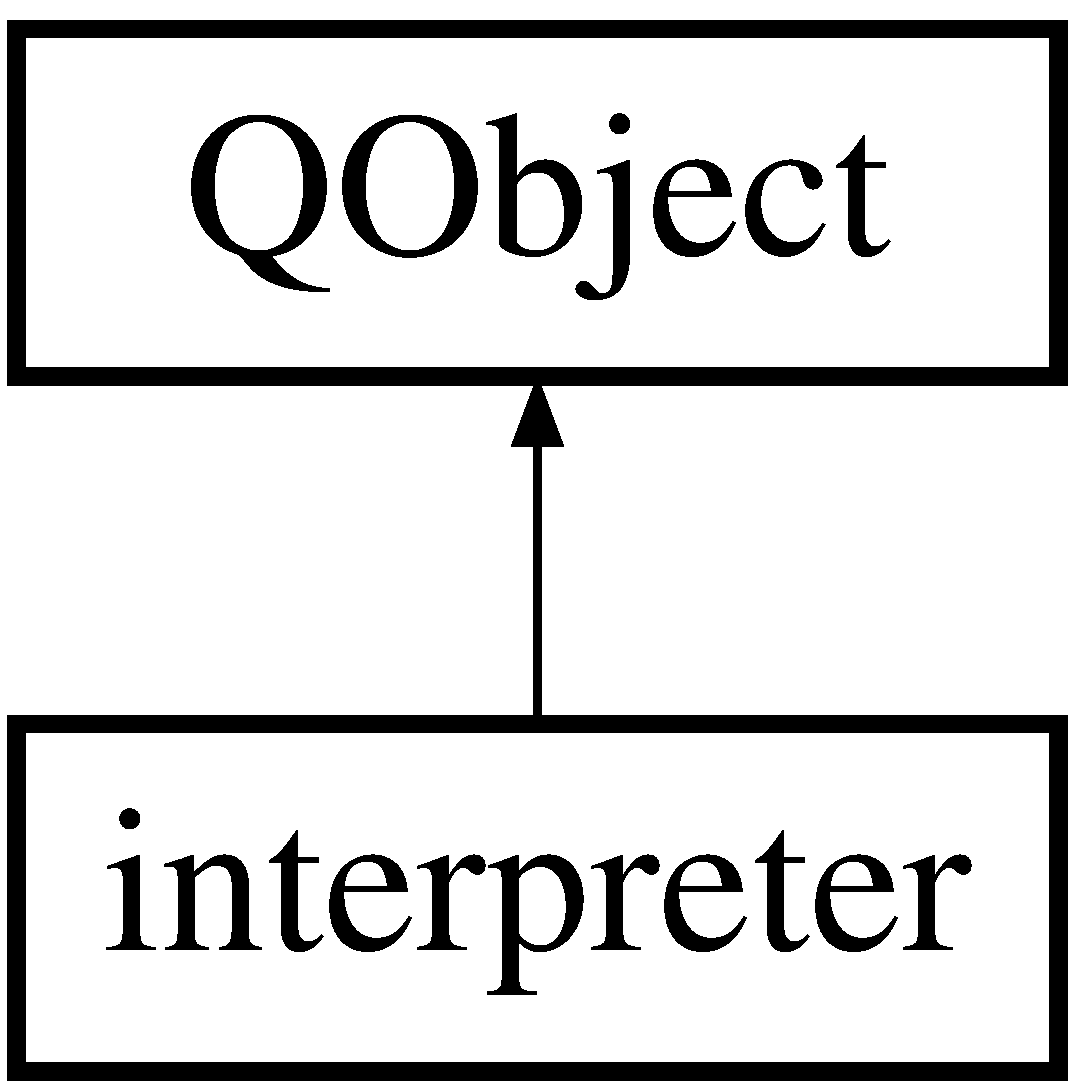
\includegraphics[height=2.000000cm]{classinterpreter}
\end{center}
\end{figure}
\subsection*{Сигналы}
\begin{DoxyCompactItemize}
\item 
\hypertarget{classinterpreter_a60e0781065c7ae88bdcaaa22729dc458}{}\label{classinterpreter_a60e0781065c7ae88bdcaaa22729dc458} 
void \hyperlink{classinterpreter_a60e0781065c7ae88bdcaaa22729dc458}{debug\+M\+SG} (Q\+String)
\begin{DoxyCompactList}\small\item\em Сигнал для отправки сообщения в поток G\+UI. \end{DoxyCompactList}\end{DoxyCompactItemize}
\subsection*{Открытые члены}
\begin{DoxyCompactItemize}
\item 
\hyperlink{classinterpreter_ae7359f1d2aa18579a2797f49835c8671}{interpreter} (Q\+String P\+A\+TH)
\begin{DoxyCompactList}\small\item\em interpreter -\/ Конструктор класса \end{DoxyCompactList}\item 
void \hyperlink{classinterpreter_af9ed8afd864c69cfd1ec1e849b2d1542}{start\+VM} ()
\begin{DoxyCompactList}\small\item\em Интерфейс запуска интерпретатора \end{DoxyCompactList}\end{DoxyCompactItemize}
\subsection*{Закрытые члены}
\begin{DoxyCompactItemize}
\item 
Q\+String \hyperlink{classinterpreter_a30d9b904383c7b73adceeca002461431}{input\+Dialog} (Q\+String text)
\begin{DoxyCompactList}\small\item\em диалоговое окно ввод \end{DoxyCompactList}\item 
void \hyperlink{classinterpreter_a5d3ba23a48b814586dabbe2e3507b93a}{output\+Dialog} (Q\+String str)
\begin{DoxyCompactList}\small\item\em диалоговое окно вывод \end{DoxyCompactList}\item 
void \hyperlink{classinterpreter_a5153712027e3e4344f72336f8b5cfa6d}{debug} (Q\+String)
\begin{DoxyCompactList}\small\item\em Отправка сигнала с текстом сообщения в поток G\+UI. \end{DoxyCompactList}\end{DoxyCompactItemize}
\subsection*{Закрытые данные}
\begin{DoxyCompactItemize}
\item 
\hypertarget{classinterpreter_a0b900e0016eab9306c6f70e93900fe09}{}\label{classinterpreter_a0b900e0016eab9306c6f70e93900fe09} 
\hyperlink{class_computer}{Computer} $\ast$ \hyperlink{classinterpreter_a0b900e0016eab9306c6f70e93900fe09}{VM}
\begin{DoxyCompactList}\small\item\em Объект компьютер \end{DoxyCompactList}\item 
\hypertarget{classinterpreter_acafdc7a0e329a4ed0f79930ed33f52be}{}\label{classinterpreter_acafdc7a0e329a4ed0f79930ed33f52be} 
Q\+String \hyperlink{classinterpreter_acafdc7a0e329a4ed0f79930ed33f52be}{Program\+Path}
\begin{DoxyCompactList}\small\item\em Путь до файла программы \end{DoxyCompactList}\end{DoxyCompactItemize}
\subsection*{Друзья}
\begin{DoxyCompactItemize}
\item 
\hypertarget{classinterpreter_ab9eca035c1f2a85f44c28a92b53d320c}{}\label{classinterpreter_ab9eca035c1f2a85f44c28a92b53d320c} 
class {\bfseries Computer}
\end{DoxyCompactItemize}


\subsection{Подробное описание}
The interpreter class. 

Запускает виртуальную машину, посредник между G\+UI и ВМ 

\subsection{Конструктор(ы)}
\hypertarget{classinterpreter_ae7359f1d2aa18579a2797f49835c8671}{}\label{classinterpreter_ae7359f1d2aa18579a2797f49835c8671} 
\index{interpreter@{interpreter}!interpreter@{interpreter}}
\index{interpreter@{interpreter}!interpreter@{interpreter}}
\subsubsection{\texorpdfstring{interpreter()}{interpreter()}}
{\footnotesize\ttfamily interpreter\+::interpreter (\begin{DoxyParamCaption}\item[{Q\+String}]{P\+A\+TH }\end{DoxyParamCaption})\hspace{0.3cm}{\ttfamily [inline]}}



interpreter -\/ Конструктор класса 


\begin{DoxyParams}{Аргументы}
{\em P\+A\+TH} & -\/ Путь до временного файла программы для запуска \\
\hline
\end{DoxyParams}

\begin{DoxyCode}
25 : \hyperlink{classinterpreter_acafdc7a0e329a4ed0f79930ed33f52be}{ProgramPath}(PATH)\{\}
\end{DoxyCode}


\subsection{Методы}
\hypertarget{classinterpreter_a5153712027e3e4344f72336f8b5cfa6d}{}\label{classinterpreter_a5153712027e3e4344f72336f8b5cfa6d} 
\index{interpreter@{interpreter}!debug@{debug}}
\index{debug@{debug}!interpreter@{interpreter}}
\subsubsection{\texorpdfstring{debug()}{debug()}}
{\footnotesize\ttfamily void interpreter\+::debug (\begin{DoxyParamCaption}\item[{Q\+String}]{msg }\end{DoxyParamCaption})\hspace{0.3cm}{\ttfamily [private]}}



Отправка сигнала с текстом сообщения в поток G\+UI. 

\hyperlink{classinterpreter_a5153712027e3e4344f72336f8b5cfa6d}{interpreter\+::debug} -\/ Запрос на вывод сообщения от программы у G\+UI


\begin{DoxyParams}{Аргументы}
{\em msg} & -\/ сообщение \\
\hline
\end{DoxyParams}

\begin{DoxyCode}
61 \{
62     emit \hyperlink{classinterpreter_a60e0781065c7ae88bdcaaa22729dc458}{debugMSG}(\textcolor{stringliteral}{"Программа#: "} + msg);
63 \}
\end{DoxyCode}
\hypertarget{classinterpreter_a30d9b904383c7b73adceeca002461431}{}\label{classinterpreter_a30d9b904383c7b73adceeca002461431} 
\index{interpreter@{interpreter}!input\+Dialog@{input\+Dialog}}
\index{input\+Dialog@{input\+Dialog}!interpreter@{interpreter}}
\subsubsection{\texorpdfstring{input\+Dialog()}{inputDialog()}}
{\footnotesize\ttfamily Q\+String interpreter\+::input\+Dialog (\begin{DoxyParamCaption}\item[{Q\+String}]{text }\end{DoxyParamCaption})\hspace{0.3cm}{\ttfamily [private]}}



диалоговое окно ввод 

\hyperlink{classinterpreter_a30d9b904383c7b73adceeca002461431}{interpreter\+::input\+Dialog} -\/ запрос на вывод диалогового окна для ввода значения


\begin{DoxyParams}{Аргументы}
{\em text} & -\/ Текст сообшения для пользователя \\
\hline
\end{DoxyParams}
\begin{DoxyReturn}{Возвращает}
Возвращает введённую пользователем строку
\end{DoxyReturn}
Запрос на вывод диалогового окна для ввода у G\+UI. 
\begin{DoxyCode}
32 \{
33     \textcolor{keywordtype}{bool} bOk;
34     QString str = QInputDialog::getText( 0, text, \textcolor{stringliteral}{"Значение"},
35                                          QLineEdit::Normal,
36                                          \textcolor{stringliteral}{""}, &bOk );
37     \textcolor{keywordflow}{if} (bOk) \{
38         \textcolor{keywordflow}{return} str;
39     \}\textcolor{keywordflow}{else} \textcolor{keywordflow}{return} \hyperlink{classinterpreter_a30d9b904383c7b73adceeca002461431}{inputDialog}(text);
40 \}
\end{DoxyCode}
\hypertarget{classinterpreter_a5d3ba23a48b814586dabbe2e3507b93a}{}\label{classinterpreter_a5d3ba23a48b814586dabbe2e3507b93a} 
\index{interpreter@{interpreter}!output\+Dialog@{output\+Dialog}}
\index{output\+Dialog@{output\+Dialog}!interpreter@{interpreter}}
\subsubsection{\texorpdfstring{output\+Dialog()}{outputDialog()}}
{\footnotesize\ttfamily void interpreter\+::output\+Dialog (\begin{DoxyParamCaption}\item[{Q\+String}]{str }\end{DoxyParamCaption})\hspace{0.3cm}{\ttfamily [private]}}



диалоговое окно вывод 

\hyperlink{classinterpreter_a5d3ba23a48b814586dabbe2e3507b93a}{interpreter\+::output\+Dialog} -\/ запрос на вывод диалогового окна для вывода сообщения


\begin{DoxyParams}{Аргументы}
{\em str} & -\/ текст сообщения\\
\hline
\end{DoxyParams}
Запрос на вывод диалогового окна с сообщением для пользователя из G\+UI 
\begin{DoxyCode}
49 \{
50     QMessageBox message;
51     message.setWindowTitle(\textcolor{stringliteral}{"Сообщение"});
52     message.setText(str);
53     message.exec();
54 \}
\end{DoxyCode}
\hypertarget{classinterpreter_af9ed8afd864c69cfd1ec1e849b2d1542}{}\label{classinterpreter_af9ed8afd864c69cfd1ec1e849b2d1542} 
\index{interpreter@{interpreter}!start\+VM@{start\+VM}}
\index{start\+VM@{start\+VM}!interpreter@{interpreter}}
\subsubsection{\texorpdfstring{start\+V\+M()}{startVM()}}
{\footnotesize\ttfamily void interpreter\+::start\+VM (\begin{DoxyParamCaption}{ }\end{DoxyParamCaption})}



Интерфейс запуска интерпретатора 

\hyperlink{classinterpreter_af9ed8afd864c69cfd1ec1e849b2d1542}{interpreter\+::start\+VM} -\/ Запуск интерпретатора

Отправка отладочных ссобщений. Инициализация и запуск вртуальной машины. 
\begin{DoxyCode}
14 \{
15      \hyperlink{classinterpreter_a0b900e0016eab9306c6f70e93900fe09}{VM} = \textcolor{keyword}{new} \hyperlink{class_computer}{Computer}(\hyperlink{classinterpreter_acafdc7a0e329a4ed0f79930ed33f52be}{ProgramPath},\textcolor{keyword}{this});
16      emit \hyperlink{classinterpreter_a60e0781065c7ae88bdcaaa22729dc458}{debugMSG}(\textcolor{stringliteral}{"Запуск программы "} + \hyperlink{classinterpreter_acafdc7a0e329a4ed0f79930ed33f52be}{ProgramPath});
17      \textcolor{keywordtype}{int} result = \hyperlink{classinterpreter_a0b900e0016eab9306c6f70e93900fe09}{VM}->\hyperlink{class_computer_a4303af6a549fc8f792de0d2d18a9e05f}{execute}();
18 
19      emit \hyperlink{classinterpreter_a60e0781065c7ae88bdcaaa22729dc458}{debugMSG}(\textcolor{stringliteral}{"Программа завершилась с кодом "} +
20                    QString::number(result) + \textcolor{stringliteral}{"\(\backslash\)n\(\backslash\)n"});
21      \textcolor{keyword}{delete} \textcolor{keyword}{this};
22 \}
\end{DoxyCode}


Объявления и описания членов классов находятся в файлах\+:\begin{DoxyCompactItemize}
\item 
C\+:/\+Users/sstarkov/\+Documents/kr\+\_\+\+Interpreter\+V\+M/sources/interpreter.\+h\item 
C\+:/\+Users/sstarkov/\+Documents/kr\+\_\+\+Interpreter\+V\+M/sources/interpreter.\+cpp\end{DoxyCompactItemize}

\hypertarget{class_main_window}{}\section{Класс Main\+Window}
\label{class_main_window}\index{Main\+Window@{Main\+Window}}


The \hyperlink{class_main_window}{Main\+Window} class -\/ G\+UI форма программы  




{\ttfamily \#include $<$mainwindow.\+h$>$}

Граф наследования\+:Main\+Window\+:\begin{figure}[H]
\begin{center}
\leavevmode
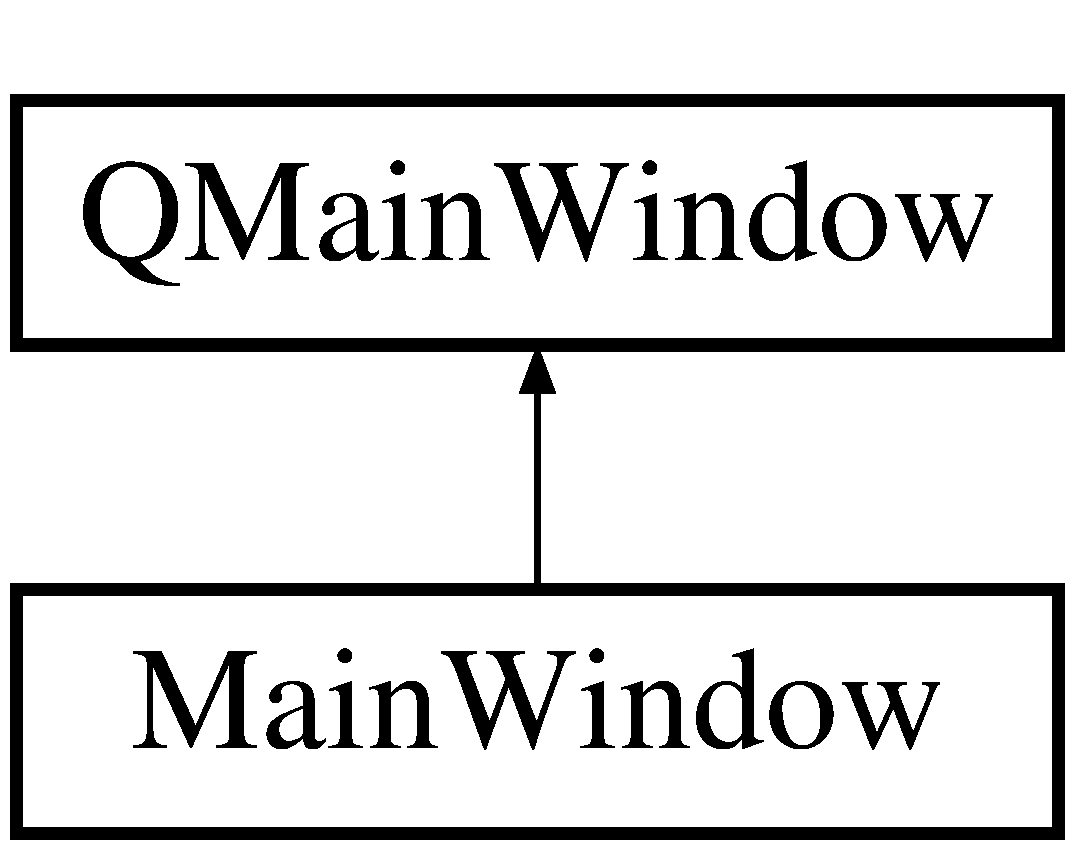
\includegraphics[height=2.000000cm]{class_main_window}
\end{center}
\end{figure}
\subsection*{Открытые члены}
\begin{DoxyCompactItemize}
\item 
\hypertarget{class_main_window_a8b244be8b7b7db1b08de2a2acb9409db}{}\label{class_main_window_a8b244be8b7b7db1b08de2a2acb9409db} 
\hyperlink{class_main_window_a8b244be8b7b7db1b08de2a2acb9409db}{Main\+Window} (Q\+Widget $\ast$parent=0)
\begin{DoxyCompactList}\small\item\em Конструктор класса формы QT. \end{DoxyCompactList}\end{DoxyCompactItemize}
\subsection*{Закрытые слоты}
\begin{DoxyCompactItemize}
\item 
void \hyperlink{class_main_window_a4b11549301823f52f40c90715cc70ec5}{on\+\_\+start\+Interpereter\+\_\+clicked} ()
\begin{DoxyCompactList}\small\item\em Запуск интерпретатора \end{DoxyCompactList}\item 
void \hyperlink{class_main_window_a06fb14e8cace4221ee7a721c961934ce}{on\+\_\+save\+\_\+clicked} ()
\begin{DoxyCompactList}\small\item\em Сохранить \end{DoxyCompactList}\item 
void \hyperlink{class_main_window_ad157e69c40c80314586029f2a7c5e549}{on\+\_\+open\+File\+\_\+clicked} ()
\begin{DoxyCompactList}\small\item\em Открыть файл \end{DoxyCompactList}\item 
void \hyperlink{class_main_window_a55dfc7c049679ca635f6f629d5401d56}{on\+\_\+\+Save\+As\+\_\+clicked} ()
\begin{DoxyCompactList}\small\item\em Сохранить как \end{DoxyCompactList}\item 
void \hyperlink{class_main_window_ac29732293ed85bb092764df7b93fefbc}{debug\+Message} (Q\+String)
\begin{DoxyCompactList}\small\item\em Вывод сообщений на форму \end{DoxyCompactList}\item 
void \hyperlink{class_main_window_a123b5275e6bb8411973a2f2be7b8b45f}{stop\+Interpreter} ()
\begin{DoxyCompactList}\small\item\em Высвобождение ресурсов, закрытие потока \end{DoxyCompactList}\end{DoxyCompactItemize}
\subsection*{Закрытые члены}
\begin{DoxyCompactItemize}
\item 
void \hyperlink{class_main_window_abc114bfc2f3b523486d89887e7877aea}{load\+File} ()
\begin{DoxyCompactList}\small\item\em Вывод файла в редактор \end{DoxyCompactList}\end{DoxyCompactItemize}
\subsection*{Закрытые данные}
\begin{DoxyCompactItemize}
\item 
\hypertarget{class_main_window_aa16438ee9c972be8c7231f2d376dafb7}{}\label{class_main_window_aa16438ee9c972be8c7231f2d376dafb7} 
Q\+Thread $\ast$ \hyperlink{class_main_window_aa16438ee9c972be8c7231f2d376dafb7}{V\+M\+Thread}
\begin{DoxyCompactList}\small\item\em Поток для интерпретатора \end{DoxyCompactList}\item 
\hypertarget{class_main_window_ab42a1f6ee7d167221b9b5078b2ba38a7}{}\label{class_main_window_ab42a1f6ee7d167221b9b5078b2ba38a7} 
\hyperlink{classinterpreter}{interpreter} $\ast$ \hyperlink{class_main_window_ab42a1f6ee7d167221b9b5078b2ba38a7}{Interpreter}
\begin{DoxyCompactList}\small\item\em Объект интерпретатора \end{DoxyCompactList}\item 
\hypertarget{class_main_window_a35466a70ed47252a0191168126a352a5}{}\label{class_main_window_a35466a70ed47252a0191168126a352a5} 
Ui\+::\+Main\+Window $\ast$ \hyperlink{class_main_window_a35466a70ed47252a0191168126a352a5}{ui}
\begin{DoxyCompactList}\small\item\em Объект формы QT. \end{DoxyCompactList}\end{DoxyCompactItemize}


\subsection{Подробное описание}
The \hyperlink{class_main_window}{Main\+Window} class -\/ G\+UI форма программы 

\subsection{Методы}
\hypertarget{class_main_window_ac29732293ed85bb092764df7b93fefbc}{}\label{class_main_window_ac29732293ed85bb092764df7b93fefbc} 
\index{Main\+Window@{Main\+Window}!debug\+Message@{debug\+Message}}
\index{debug\+Message@{debug\+Message}!Main\+Window@{Main\+Window}}
\subsubsection{\texorpdfstring{debug\+Message}{debugMessage}}
{\footnotesize\ttfamily void Main\+Window\+::debug\+Message (\begin{DoxyParamCaption}\item[{Q\+String}]{str }\end{DoxyParamCaption})\hspace{0.3cm}{\ttfamily [private]}, {\ttfamily [slot]}}



Вывод сообщений на форму 

\hyperlink{class_main_window_ac29732293ed85bb092764df7b93fefbc}{Main\+Window\+::debug\+Message} -\/ вывод сообщения на форму


\begin{DoxyParams}{Аргументы}
{\em str} & -\/ текст сообщения \\
\hline
\end{DoxyParams}

\begin{DoxyCode}
122 \{
123     \hyperlink{class_main_window_a35466a70ed47252a0191168126a352a5}{ui}->debugLog->append(str);
124 \}
\end{DoxyCode}
\hypertarget{class_main_window_abc114bfc2f3b523486d89887e7877aea}{}\label{class_main_window_abc114bfc2f3b523486d89887e7877aea} 
\index{Main\+Window@{Main\+Window}!load\+File@{load\+File}}
\index{load\+File@{load\+File}!Main\+Window@{Main\+Window}}
\subsubsection{\texorpdfstring{load\+File()}{loadFile()}}
{\footnotesize\ttfamily void Main\+Window\+::load\+File (\begin{DoxyParamCaption}{ }\end{DoxyParamCaption})\hspace{0.3cm}{\ttfamily [private]}}



Вывод файла в редактор 

\hyperlink{class_main_window_abc114bfc2f3b523486d89887e7877aea}{Main\+Window\+::load\+File} -\/ Загрузка файла

Загружает файл программы для предпросмотра программы 
\begin{DoxyCode}
23 \{
24     QString text, path;
25     path = \hyperlink{class_main_window_a35466a70ed47252a0191168126a352a5}{ui}->pathToFile->text();
26     QFile file(path);
27     \textcolor{keywordflow}{if}(file.open(QIODevice::ReadOnly | QIODevice::Text))\{
28         text = file.readAll();
29     \}
30     \textcolor{keywordflow}{else} \{
31         QMessageBox m; m.setText(\textcolor{stringliteral}{"Не удалось открыть файл: "} + path); m.exec();
32     \}
33     \textcolor{keywordflow}{if}(file.isOpen()) file.close();
34     \hyperlink{class_main_window_a35466a70ed47252a0191168126a352a5}{ui}->programText->setText(text);
35 \}
\end{DoxyCode}
\hypertarget{class_main_window_ad157e69c40c80314586029f2a7c5e549}{}\label{class_main_window_ad157e69c40c80314586029f2a7c5e549} 
\index{Main\+Window@{Main\+Window}!on\+\_\+open\+File\+\_\+clicked@{on\+\_\+open\+File\+\_\+clicked}}
\index{on\+\_\+open\+File\+\_\+clicked@{on\+\_\+open\+File\+\_\+clicked}!Main\+Window@{Main\+Window}}
\subsubsection{\texorpdfstring{on\+\_\+open\+File\+\_\+clicked}{on\_openFile\_clicked}}
{\footnotesize\ttfamily void Main\+Window\+::on\+\_\+open\+File\+\_\+clicked (\begin{DoxyParamCaption}{ }\end{DoxyParamCaption})\hspace{0.3cm}{\ttfamily [private]}, {\ttfamily [slot]}}



Открыть файл 

\hyperlink{class_main_window_ad157e69c40c80314586029f2a7c5e549}{Main\+Window\+::on\+\_\+open\+File\+\_\+clicked} -\/ форма для выбора файла для открытия 
\begin{DoxyCode}
108 \{
109     QString path = QFileDialog::getOpenFileName(\textcolor{keyword}{this},
110                                 QString::fromUtf8(\textcolor{stringliteral}{"Открыть файл"}),
111                                 QDir::currentPath(),
112                                 \textcolor{stringliteral}{"Text (*.txt);"});
113     \hyperlink{class_main_window_a35466a70ed47252a0191168126a352a5}{ui}->pathToFile->setText(path);
114     \textcolor{keywordflow}{if}(!path.isEmpty()) \hyperlink{class_main_window_abc114bfc2f3b523486d89887e7877aea}{loadFile}();
115 \}
\end{DoxyCode}
\hypertarget{class_main_window_a06fb14e8cace4221ee7a721c961934ce}{}\label{class_main_window_a06fb14e8cace4221ee7a721c961934ce} 
\index{Main\+Window@{Main\+Window}!on\+\_\+save\+\_\+clicked@{on\+\_\+save\+\_\+clicked}}
\index{on\+\_\+save\+\_\+clicked@{on\+\_\+save\+\_\+clicked}!Main\+Window@{Main\+Window}}
\subsubsection{\texorpdfstring{on\+\_\+save\+\_\+clicked}{on\_save\_clicked}}
{\footnotesize\ttfamily void Main\+Window\+::on\+\_\+save\+\_\+clicked (\begin{DoxyParamCaption}{ }\end{DoxyParamCaption})\hspace{0.3cm}{\ttfamily [private]}, {\ttfamily [slot]}}



Сохранить 

\hyperlink{class_main_window_a06fb14e8cace4221ee7a721c961934ce}{Main\+Window\+::on\+\_\+save\+\_\+clicked} Сохранить файл

Сохраняет файл из текстового редактора 
\begin{DoxyCode}
91 \{
92     QString path;
93     path = \hyperlink{class_main_window_a35466a70ed47252a0191168126a352a5}{ui}->pathToFile->text();
94     QFile file(path);
95     \textcolor{keywordflow}{if}(file.open(QIODevice::WriteOnly | QIODevice::Text))
96     \{
97         QByteArray ba;
98         ba.append(\hyperlink{class_main_window_a35466a70ed47252a0191168126a352a5}{ui}->programText->toPlainText());
99         file.write(ba);
100     \}
101     \textcolor{keywordflow}{if}(file.isOpen()) file.close();
102 \}
\end{DoxyCode}
\hypertarget{class_main_window_a55dfc7c049679ca635f6f629d5401d56}{}\label{class_main_window_a55dfc7c049679ca635f6f629d5401d56} 
\index{Main\+Window@{Main\+Window}!on\+\_\+\+Save\+As\+\_\+clicked@{on\+\_\+\+Save\+As\+\_\+clicked}}
\index{on\+\_\+\+Save\+As\+\_\+clicked@{on\+\_\+\+Save\+As\+\_\+clicked}!Main\+Window@{Main\+Window}}
\subsubsection{\texorpdfstring{on\+\_\+\+Save\+As\+\_\+clicked}{on\_SaveAs\_clicked}}
{\footnotesize\ttfamily void Main\+Window\+::on\+\_\+\+Save\+As\+\_\+clicked (\begin{DoxyParamCaption}{ }\end{DoxyParamCaption})\hspace{0.3cm}{\ttfamily [private]}, {\ttfamily [slot]}}



Сохранить как 

\hyperlink{class_main_window_a55dfc7c049679ca635f6f629d5401d56}{Main\+Window\+::on\+\_\+\+Save\+As\+\_\+clicked} -\/ Сохранить как?

Открытие формы для указания имени файла для сохраниения 
\begin{DoxyCode}
132 \{
133     QString path = QFileDialog::getSaveFileName(\textcolor{keyword}{this},
134                                 QString::fromUtf8(\textcolor{stringliteral}{"Сохранить файл"}),
135                                 QDir::currentPath(),
136                                 \textcolor{stringliteral}{"Text (*.txt);"});
137     \hyperlink{class_main_window_a35466a70ed47252a0191168126a352a5}{ui}->pathToFile->setText(path);
138     \hyperlink{class_main_window_a06fb14e8cace4221ee7a721c961934ce}{on\_save\_clicked}();
139 \}
\end{DoxyCode}
\hypertarget{class_main_window_a4b11549301823f52f40c90715cc70ec5}{}\label{class_main_window_a4b11549301823f52f40c90715cc70ec5} 
\index{Main\+Window@{Main\+Window}!on\+\_\+start\+Interpereter\+\_\+clicked@{on\+\_\+start\+Interpereter\+\_\+clicked}}
\index{on\+\_\+start\+Interpereter\+\_\+clicked@{on\+\_\+start\+Interpereter\+\_\+clicked}!Main\+Window@{Main\+Window}}
\subsubsection{\texorpdfstring{on\+\_\+start\+Interpereter\+\_\+clicked}{on\_startInterpereter\_clicked}}
{\footnotesize\ttfamily void Main\+Window\+::on\+\_\+start\+Interpereter\+\_\+clicked (\begin{DoxyParamCaption}{ }\end{DoxyParamCaption})\hspace{0.3cm}{\ttfamily [private]}, {\ttfamily [slot]}}



Запуск интерпретатора 

\hyperlink{class_main_window_a4b11549301823f52f40c90715cc70ec5}{Main\+Window\+::on\+\_\+start\+Interpereter\+\_\+clicked} -\/ Кнопка запуска инретпретатора

Сохраняет текст программы из редактора во временный файл. Инициализирует поток для интерпретатора. Запскает интерпретатор в отдельном от G\+UI потоке (в качестве файла программы выступает временный $\ast$.tmp файл). По завершении работы интерпретатора удаляет временый файл. 
\begin{DoxyCode}
46 \{    
47     \textcolor{keywordflow}{if}(\hyperlink{class_main_window_a35466a70ed47252a0191168126a352a5}{ui}->programText->toPlainText().isEmpty()) \textcolor{keywordflow}{return};
48     QString tmpPath = \hyperlink{class_main_window_a35466a70ed47252a0191168126a352a5}{ui}->pathToFile->text() + \textcolor{stringliteral}{".tmp"};
49 
50     QFile file(tmpPath);
51     \textcolor{keywordflow}{if}(file.open(QIODevice::WriteOnly | QIODevice::Text))
52     \{
53         QByteArray ba;
54         ba.append(\hyperlink{class_main_window_a35466a70ed47252a0191168126a352a5}{ui}->programText->toPlainText());
55         file.write(ba);
56     \}
57     \textcolor{keywordflow}{if}(file.isOpen()) file.close();
58 
59     \textcolor{comment}{//старт интерпретатора в потоке}
60     \hyperlink{class_main_window_aa16438ee9c972be8c7231f2d376dafb7}{VMThread} = \textcolor{keyword}{new} QThread();
61 
62     \hyperlink{class_main_window_ab42a1f6ee7d167221b9b5078b2ba38a7}{Interpreter} = \textcolor{keyword}{new} \hyperlink{classinterpreter}{interpreter}(tmpPath);
63     connect(\hyperlink{class_main_window_ab42a1f6ee7d167221b9b5078b2ba38a7}{Interpreter},SIGNAL(destroyed(QObject*)),\textcolor{keyword}{this},SLOT(
      \hyperlink{class_main_window_a123b5275e6bb8411973a2f2be7b8b45f}{stopInterpreter}()));
64     connect(\hyperlink{class_main_window_ab42a1f6ee7d167221b9b5078b2ba38a7}{Interpreter},SIGNAL(debugMSG(QString)),\textcolor{keyword}{this},SLOT(
      \hyperlink{class_main_window_ac29732293ed85bb092764df7b93fefbc}{debugMessage}(QString)));
65 
66     \hyperlink{class_main_window_ab42a1f6ee7d167221b9b5078b2ba38a7}{Interpreter}->moveToThread(\hyperlink{class_main_window_aa16438ee9c972be8c7231f2d376dafb7}{VMThread});
67     \hyperlink{class_main_window_aa16438ee9c972be8c7231f2d376dafb7}{VMThread}->start();
68     \hyperlink{class_main_window_ab42a1f6ee7d167221b9b5078b2ba38a7}{Interpreter}->\hyperlink{classinterpreter_af9ed8afd864c69cfd1ec1e849b2d1542}{startVM}();
69 
70     QFile(tmpPath).remove();
71 \}
\end{DoxyCode}
\hypertarget{class_main_window_a123b5275e6bb8411973a2f2be7b8b45f}{}\label{class_main_window_a123b5275e6bb8411973a2f2be7b8b45f} 
\index{Main\+Window@{Main\+Window}!stop\+Interpreter@{stop\+Interpreter}}
\index{stop\+Interpreter@{stop\+Interpreter}!Main\+Window@{Main\+Window}}
\subsubsection{\texorpdfstring{stop\+Interpreter}{stopInterpreter}}
{\footnotesize\ttfamily void Main\+Window\+::stop\+Interpreter (\begin{DoxyParamCaption}{ }\end{DoxyParamCaption})\hspace{0.3cm}{\ttfamily [private]}, {\ttfamily [slot]}}



Высвобождение ресурсов, закрытие потока 

\hyperlink{class_main_window_a123b5275e6bb8411973a2f2be7b8b45f}{Main\+Window\+::stop\+Interpreter} -\/ Завершение работы интерпретатора

Остановка потока, высвобождение ресурсов 
\begin{DoxyCode}
79 \{
80     \hyperlink{class_main_window_aa16438ee9c972be8c7231f2d376dafb7}{VMThread}->quit();
81     \hyperlink{class_main_window_aa16438ee9c972be8c7231f2d376dafb7}{VMThread}->wait(100);
82     \textcolor{keyword}{delete} \hyperlink{class_main_window_aa16438ee9c972be8c7231f2d376dafb7}{VMThread};
83 \}
\end{DoxyCode}


Объявления и описания членов классов находятся в файлах\+:\begin{DoxyCompactItemize}
\item 
C\+:/\+Users/sstarkov/\+Documents/kr\+\_\+\+Interpreter\+V\+M/sources/mainwindow.\+h\item 
C\+:/\+Users/sstarkov/\+Documents/kr\+\_\+\+Interpreter\+V\+M/sources/mainwindow.\+cpp\end{DoxyCompactItemize}

%--- End generated contents ---

% Index
\backmatter
\newpage
\phantomsection
\clearemptydoublepage
\addcontentsline{toc}{chapter}{Алфавитный указатель}
\printindex

\end{document}
